%=============================================================================
%  report_ieee14_switch_en_rev2.tex
%  Standalone English report: automatic GFL/GFM reference-mode switching in a
%  1-SG / 4-IBR IEEE-14 system. Model equations, small-signal spectrum, the
%  switched time-domain formulation, and a five-policy comparison on one
%  trajectory.
%
%  This revision supersedes report_ieee14_switch_en_new.tex. What changed:
%    - results moved from the preserved 200-s run to the 250-s adaptive arm
%      (output/diagnostics/ieee14_gfm_lock_compare/adaptive_250s.mat);
%    - the AGSI decision page and its two zoom pages were added;
%    - the disturbance-chronology diagram was moved above the result figures;
%    - the IBR state count was CORRECTED from 20 to the 16 states the run
%      actually integrates (defect TD-2026-08-12-01 reduced the two
%      command-delay states per branch by singular perturbation; the earlier
%      report text described the pre-reduction layout);
%    - a proof of the block structure of the stacked right-hand side was added;
%    - a five-arm control-policy comparison section was added.
%
%  PROVENANCE AND NUMERICAL INTEGRITY
%  - Every model equation reproduced below is transcribed from the project-owned
%    base-MATLAB production code that the 250-s chronology run executes
%    (+stability/ts_simulate_ibr_hybrid.m, +stability/composite_dae.m and the
%    +ibr / +cases packages they call). No equation is invented for the report.
%  - Every plotted sample is a raw accepted value of the 250-s accepted
%    trajectory. No signal is smoothed, filtered, decimated, offset, re-sampled
%    or augmented with synthetic noise.
%  - Every printed scalar is read through a generated macro file, so prose and
%    tables cannot drift from the run.
%  - Sourced inputs, project-derived closures, case-defined parameters and
%    numerical-method choices are labelled where they first appear.
%
%  BUILD:  xelatex report_ieee14_switch_en_rev2.tex   (run twice for references)
%=============================================================================
\documentclass[12pt,a4paper]{article}

\usepackage{graphicx,amsmath,amssymb,float,caption,hyperref,fancyhdr}
% amsthm MUST precede newtxmath: both define \openbox, and newtx tolerates the
% clash only in this order.
\usepackage{amsthm}
\usepackage{newtxtext,newtxmath}
\newtheorem{proposition}{Proposition}
\newtheorem{corollary}{Corollary}
\theoremstyle{remark}
\newtheorem{remark}{Remark}
\usepackage{geometry,booktabs,tabularx,array,longtable,microtype}
\usepackage{xcolor}
\usepackage{tikz}
\usetikzlibrary{arrows.meta,positioning,calc}
\geometry{margin=1in}
\setlength{\headheight}{14.5pt}
\pagestyle{fancy}
\fancyhf{}
\lhead{IEEE-14  GFL/GFM  switching}
\rhead{\thepage}
\renewcommand{\headrulewidth}{0.4pt}
\renewcommand{\arraystretch}{1.12}
\emergencystretch=1.5em
\hypersetup{colorlinks=true,linkcolor=blue!45!black,citecolor=blue!45!black,
  urlcolor=blue!45!black}

\DeclareMathOperator{\sat}{sat}
\newcommand{\pu}{\,\mathrm{p.u.}}
\newcommand{\second}{\,\mathrm{s}}

% Graphics search path (report lives in docs/source/).
\graphicspath{{figures/}{figures/switch_ieee14_decision/}{figures/switch_ieee14/}{figures/switch_ieee14_new/}}

% Run scalars of the 250-s adaptive arm (\New*-prefixed), written by
%   pf_init_paths; generate_ieee14_report_scalars
% from output/diagnostics/ieee14_gfm_lock_compare/adaptive_250s.mat. The macro
% NAMES are unchanged from the earlier 200-s file, so the body text below moved
% onto the new run without a single edit to a number: prose and tables read the
% macros, never a literal. Guarded so the document still builds before the figure
% pipeline has run.
\IfFileExists{figures/switch_ieee14_decision/run_summary_v2.tex}
  {% Generated by generate_ieee14_report_scalars. Do not edit.
%
% PROVENANCE. Accepted values of output/diagnostics/ieee14_gfm_lock_compare_dcreal/adaptive_250s.mat.
% Produced by run_ieee14_gfm_lock_comparison, whose option set is the
% flagship driver's plus agsi_reference=true (opt-in, post-processing only).
% This cache is NOT bit-identical to the earlier delivered artifact, and no
% such claim is made for it: the DC-link closure changed under
% NUM-2026-08-20-01, so the trajectory legitimately differs. Compare it to
% the earlier cache by outcome, never by bit-identity.
% No value here is rounded, scaled, smoothed or otherwise altered.
%
% Regenerate with:  pf_init_paths; generate_ieee14_report_scalars(result_file="output/diagnostics/ieee14_gfm_lock_compare_dcreal/adaptive_250s.mat")

\newcommand{\NewRunEnd}{250.000}
\newcommand{\NewRunVMin}{0.036855}
\newcommand{\NewRunVMax}{1.523183}
\newcommand{\NewRunFMin}{58.838795}
\newcommand{\NewRunFMax}{61.138560}
\newcommand{\NewRunSubdivision}{0}
\newcommand{\NewRunDomainRejects}{584}
\newcommand{\NewRunResidual}{$9.9596\times10^{-9}$}
\newcommand{\NewRunReclose}{159.240}
\newcommand{\NewRunRecloseStatus}{SUCCESS}
\newcommand{\NewRunSyncDV}{0.008785}
\newcommand{\NewRunSyncDF}{$6.4601\times10^{-13}$}
\newcommand{\NewRunSyncDTheta}{5.015017}
\newcommand{\NewRunFirstRelease}{25.310}
\newcommand{\NewRunReleaseOne}{25.310}
\newcommand{\NewRunReleaseTwo}{146.247}
\newcommand{\NewRunReleaseThree}{152.390}
\newcommand{\NewRunReleaseFour}{--}
\newcommand{\NewRunAugmentOne}{22.052}
\newcommand{\NewRunAugmentTwo}{51.333}
\newcommand{\NewRunAugmentThree}{53.372}
\newcommand{\NewRunAugmentFour}{148.267}
\newcommand{\NewRunNRelease}{3}
\newcommand{\NewRunNAugment}{4}
\newcommand{\NewRunGfmMax}{4}
\newcommand{\NewRunSamples}{4990}
\newcommand{\NewRunRejectedSteps}{135}
\newcommand{\NewRunTerminalF}{60.000000}
\newcommand{\NewRunTerminalVMin}{0.9667}
\newcommand{\NewRunTerminalVMax}{1.0575}
\newcommand{\NewRunStepper}{adaptive}
\newcommand{\NewRunReselection}{NO\_FEASIBLE\_SG\_ON\_ONE\_STEP}
}
  {\newcommand{\NewRunEnd}{250.000}\newcommand{\NewRunVMin}{--}%
   \newcommand{\NewRunVMax}{--}\newcommand{\NewRunFMin}{--}%
   \newcommand{\NewRunFMax}{--}\newcommand{\NewRunSubdivision}{--}%
   \newcommand{\NewRunDomainRejects}{--}\newcommand{\NewRunResidual}{--}%
   \newcommand{\NewRunReclose}{--}\newcommand{\NewRunFirstRelease}{--}%
   \newcommand{\NewRunReleaseOne}{--}\newcommand{\NewRunReleaseTwo}{--}%
   \newcommand{\NewRunReleaseThree}{--}\newcommand{\NewRunReleaseFour}{--}%
   \newcommand{\NewRunSyncDV}{--}\newcommand{\NewRunSyncDF}{--}%
   \newcommand{\NewRunSyncDTheta}{--}\newcommand{\NewRunRecloseStatus}{--}%
   \newcommand{\NewRunAugmentOne}{--}\newcommand{\NewRunAugmentTwo}{--}%
   \newcommand{\NewRunAugmentThree}{--}\newcommand{\NewRunAugmentFour}{--}%
   \newcommand{\NewRunNRelease}{--}\newcommand{\NewRunNAugment}{--}%
   \newcommand{\NewRunGfmMax}{--}\newcommand{\NewRunSamples}{--}%
   \newcommand{\NewRunRejectedSteps}{--}\newcommand{\NewRunTerminalF}{--}%
   \newcommand{\NewRunTerminalVMin}{--}\newcommand{\NewRunTerminalVMax}{--}%
   \newcommand{\NewRunStepper}{--}\newcommand{\NewRunReselection}{--}}

% Cross-arm comparison macros, written by
%   pf_init_paths; generate_ieee14_gfm_lock_comparison
% Every number the comparison section prints comes from here, so the prose cannot
% drift from the runs. Guarded the same way.
\IfFileExists{figures/switch_ieee14_decision/comparison_macros.tex}
  {% Generated by generate_ieee14_gfm_lock_comparison. Do not edit.
% Every number the comparison section prints comes from here, so the prose cannot drift
% from the runs. Arm keys: adaptive, pinned_gfm1, pinned_gfm2, pinned_gfm4, locked_gfl

\newcommand{\ArmAdaptiveLabel}{adaptive}
\newcommand{\ArmAdaptiveHorizon}{250.000}
\newcommand{\ArmAdaptiveConverged}{1}
\newcommand{\ArmAdaptiveReclose}{159.2397}
\newcommand{\ArmAdaptiveGfmMax}{4}
\newcommand{\ArmAdaptiveFailure}{--}
\newcommand{\ArmAdaptiveSamples}{4990}
\newcommand{\ArmAdaptiveRejected}{135}
\newcommand{\DfAdaptiveSGtrip}{0.7587}
\newcommand{\SetAdaptiveSGtrip}{0.0041}
\newcommand{\DfAdaptiveLoadstep}{1.0035}
\newcommand{\SetAdaptiveLoadstep}{0.3753}
\newcommand{\DfAdaptiveFault}{1.1386}
\newcommand{\SetAdaptiveFault}{0.3753}
\newcommand{\DfAdaptiveLinetrip}{0.3764}
\newcommand{\SetAdaptiveLinetrip}{0.3503}
\newcommand{\DfAdaptiveRestorereclose}{1.1612}
\newcommand{\SetAdaptiveRestorereclose}{0.0130}
\newcommand{\ArmPinnedgfmOneLabel}{pinned 1 GFM}
\newcommand{\ArmPinnedgfmOneHorizon}{250.000}
\newcommand{\ArmPinnedgfmOneConverged}{1}
\newcommand{\ArmPinnedgfmOneReclose}{151.4244}
\newcommand{\ArmPinnedgfmOneGfmMax}{1}
\newcommand{\ArmPinnedgfmOneFailure}{--}
\newcommand{\ArmPinnedgfmOneSamples}{3232}
\newcommand{\ArmPinnedgfmOneRejected}{542}
\newcommand{\DfPinnedgfmOneSGtrip}{0.5312}
\newcommand{\SetPinnedgfmOneSGtrip}{0.0113}
\newcommand{\DfPinnedgfmOneLoadstep}{1.4478}
\newcommand{\SetPinnedgfmOneLoadstep}{1.2214}
\newcommand{\DfPinnedgfmOneFault}{1.4979}
\newcommand{\SetPinnedgfmOneFault}{1.2296}
\newcommand{\DfPinnedgfmOneLinetrip}{1.2325}
\newcommand{\SetPinnedgfmOneLinetrip}{1.1426}
\newcommand{\DfPinnedgfmOneRestorereclose}{1.1736}
\newcommand{\SetPinnedgfmOneRestorereclose}{0.0210}
\newcommand{\ArmPinnedgfmTwoLabel}{pinned 2 GFM}
\newcommand{\ArmPinnedgfmTwoHorizon}{250.000}
\newcommand{\ArmPinnedgfmTwoConverged}{1}
\newcommand{\ArmPinnedgfmTwoReclose}{149.9191}
\newcommand{\ArmPinnedgfmTwoGfmMax}{2}
\newcommand{\ArmPinnedgfmTwoFailure}{--}
\newcommand{\ArmPinnedgfmTwoSamples}{3183}
\newcommand{\ArmPinnedgfmTwoRejected}{321}
\newcommand{\DfPinnedgfmTwoSGtrip}{0.3489}
\newcommand{\SetPinnedgfmTwoSGtrip}{0.0001}
\newcommand{\DfPinnedgfmTwoLoadstep}{0.7839}
\newcommand{\SetPinnedgfmTwoLoadstep}{0.7123}
\newcommand{\DfPinnedgfmTwoFault}{0.8255}
\newcommand{\SetPinnedgfmTwoFault}{0.7126}
\newcommand{\DfPinnedgfmTwoLinetrip}{0.7135}
\newcommand{\SetPinnedgfmTwoLinetrip}{0.6422}
\newcommand{\DfPinnedgfmTwoRestorereclose}{0.6634}
\newcommand{\SetPinnedgfmTwoRestorereclose}{0.0209}
\newcommand{\ArmPinnedgfmFourLabel}{pinned 4 GFM}
\newcommand{\ArmPinnedgfmFourHorizon}{25.491}
\newcommand{\ArmPinnedgfmFourConverged}{0}
\newcommand{\ArmPinnedgfmFourReclose}{--}
\newcommand{\ArmPinnedgfmFourGfmMax}{4}
\newcommand{\ArmPinnedgfmFourFailure}{\texttt{adaptiveDtMin}}
\newcommand{\ArmPinnedgfmFourSamples}{819}
\newcommand{\ArmPinnedgfmFourRejected}{449}
\newcommand{\DfPinnedgfmFourSGtrip}{0.9898}
\newcommand{\SetPinnedgfmFourSGtrip}{--}
\newcommand{\DfPinnedgfmFourLoadstep}{--}
\newcommand{\SetPinnedgfmFourLoadstep}{--}
\newcommand{\DfPinnedgfmFourFault}{--}
\newcommand{\SetPinnedgfmFourFault}{--}
\newcommand{\DfPinnedgfmFourLinetrip}{--}
\newcommand{\SetPinnedgfmFourLinetrip}{--}
\newcommand{\DfPinnedgfmFourRestorereclose}{--}
\newcommand{\SetPinnedgfmFourRestorereclose}{--}
\newcommand{\ArmLockedgflLabel}{locked GFL}
\newcommand{\ArmLockedgflHorizon}{20.000}
\newcommand{\ArmLockedgflConverged}{0}
\newcommand{\ArmLockedgflReclose}{--}
\newcommand{\ArmLockedgflGfmMax}{0}
\newcommand{\ArmLockedgflFailure}{\texttt{noVoltageFormingSource}}
\newcommand{\ArmLockedgflSamples}{43}
\newcommand{\ArmLockedgflRejected}{0}
\newcommand{\DfLockedgflSGtrip}{--}
\newcommand{\SetLockedgflSGtrip}{--}
\newcommand{\DfLockedgflLoadstep}{--}
\newcommand{\SetLockedgflLoadstep}{--}
\newcommand{\DfLockedgflFault}{--}
\newcommand{\SetLockedgflFault}{--}
\newcommand{\DfLockedgflLinetrip}{--}
\newcommand{\SetLockedgflLinetrip}{--}
\newcommand{\DfLockedgflRestorereclose}{--}
\newcommand{\SetLockedgflRestorereclose}{--}
\newcommand{\CommonWindowPinnedgfmOneBitIdentical}{1}
\newcommand{\CommonWindowPinnedgfmOneSamples}{42}
\newcommand{\CommonWindowPinnedgfmTwoBitIdentical}{1}
\newcommand{\CommonWindowPinnedgfmTwoSamples}{42}
\newcommand{\CommonWindowPinnedgfmFourBitIdentical}{1}
\newcommand{\CommonWindowPinnedgfmFourSamples}{42}
\newcommand{\CommonWindowLockedgflBitIdentical}{1}
\newcommand{\CommonWindowLockedgflSamples}{42}
\newcommand{\CommonWindowSplit}{20.000}
\newcommand{\CommonWindowAllBitIdentical}{1}
\newcommand{\CandTotal}{15}
\newcommand{\CandReady}{7}
\newcommand{\CandBestSet}{IBR3+IBR6}
\newcommand{\CandBestN}{2}
\newcommand{\CandBestOmega}{-0.56814}
\newcommand{\CandBestSingleOmega}{-0.32801}
\newcommand{\CandFullOmega}{-0.48291}
\newcommand{\CandReadyNOne}{4}
\newcommand{\CandTotalNOne}{4}
\newcommand{\CandReadyNTwo}{2}
\newcommand{\CandTotalNTwo}{6}
\newcommand{\CandReadyNThree}{0}
\newcommand{\CandTotalNThree}{4}
\newcommand{\CandReadyNFour}{1}
\newcommand{\CandTotalNFour}{1}
}
  {}

% Period colours for the disturbance-chronology diagram.
\definecolor{pgreen}{RGB}{41,153,69}
\definecolor{pred}{RGB}{191,45,45}
\definecolor{pblue}{RGB}{46,107,191}
\definecolor{pyellow}{RGB}{199,178,38}
\definecolor{pgrey}{RGB}{90,90,90}

\title{\bfseries Automatic GFL/GFM Reference-Mode Switching in a
1-SG / 4-IBR IEEE-14 System:\\[2pt]
\large Model, Small-Signal Spectrum, Switched Time-Domain Formulation,\\
and a Five-Policy Comparison on One Trajectory\\[2pt]
\normalsize ($\NewRunEnd\second$ result set)}
\author{Power-flow / stability toolchain --- generated report}
\date{}

\begin{document}
\maketitle
\thispagestyle{fancy}

\begin{abstract}
\noindent
A modified IEEE-14 network is driven through a six-period chronology in which a
single synchronous generator (SG) is tripped, the load is stepped, a shunt fault
is applied and cleared, a tie line is opened, and the SG is finally reclosed.
Four inverter-based resources (IBRs) switch \emph{automatically} between
grid-following (GFL) and grid-forming (GFM) reference behaviour under an
amplitude--frequency severity index with hysteresis and dwell. This report
documents, from the production code, (i) the severity index and its two
component sub-indices $J_V,J_f$, together with the four reference-only
diagnostic indices published alongside them; (ii) the sixth-order SG model with
an order-by-order derivation and the singular limit that freezes one flux state;
(iii) the sixteen-state dual-mode IBR superset with its active projections and
current-continuity-gated transfer; (iv) the switched implicit-trapezoidal
time-domain formulation, including a proof of the block structure of the stacked
right-hand side and the exact mechanism by which an integrated state update is
replaced by a discrete transfer at a mode change; (v) the solved power flow, the
small-signal spectrum, and the accepted transient response of the
$\NewRunEnd\second$ run; and (vi) a comparison of \emph{five} control policies
--- all-GFL locked, one, two and four pinned grid-forming units, and the
delivered adaptive supervisor --- on the same network, dispatch, event schedule
and solver. All equations are those the run executes; all plotted curves are raw
accepted samples of that run. No claim of operational readiness is made:
convergence of the simulation is not evidence of grid-code compliance.
\end{abstract}

\tableofcontents

%=============================================================================
\section{Introduction}\label{sec:intro}
%=============================================================================
Displacing synchronous machines with converter-interfaced generation removes
rotating inertia from the system, and the consequences for frequency stability are
by now well characterised: the review in~\cite{he2024} surveys the mechanisms and
the control responses, \cite{zhang2025} proposes a quantitative inertia-security
assessment for exactly this regime, and \cite{nema2022} is one of many synthetic
inertia schemes that answer the shortfall from the converter side. What that
literature makes clear is that the shortfall is not only a matter of how much
inertia is emulated, but of \emph{which converters are willing to form a voltage}
when the last machine leaves.

Grid-forming (GFM) control answers that question by making the converter a voltage
source with its own angle, the mode whose autonomous operation was characterised
early for inverter-based microgrids~\cite{pogaku2007}, and grid-following (GFL) control declines it by
synchronising to a measured angle through a phase-locked loop. Neither is free.
GFM requires active and reactive headroom to be reserved, which is why
\cite{cui2025} treats the control mode as a dispatchable grid service with a
steady-state cost rather than as a fixed property of a device, and why the
capability envelope of a grid-forming inverter has needed explicit
characterisation~\cite{nurunnabi2025}. Under a fault, the two modes behave
differently once the current limit binds~\cite{almesri2025}, which is where the
comparison stops being a matter of taste.

That cost is what motivates \emph{switching} rather than choosing. Designs that let
one converter present either behaviour have been proposed with minimal structural
change~\cite{ding2025}, adapted continuously to the short-circuit
ratio~\cite{liu2024}, made bumpless at the transition~\cite{gao2025}, or unified
into a single grid-following framework that also survives weak
grids~\cite{askarian2024}. In parallel, the transient behaviour of systems that
mix machines with both converter types has been analysed directly: \cite{he2022}
for inverter-based generation against a machine, \cite{qu2025} for the damping
interaction in a hybrid GFL-GFM pair, \cite{chen2025} for a parallel
SG-GFL-GFM system, and---closest to the mechanism this report ends up
measuring---\cite{li2026}, which studies what the \emph{switching of}
droop-controlled grid-forming converters does to the transient stability of the
grid-following converters around them.

\paragraph{What is not settled by that work.}
Those studies establish that switching helps and that mixed systems have coupled
transient behaviour. They do not, between them, answer the question a system
operator actually faces on a multi-machine network: given a set of converters that
\emph{could} form a voltage, how many should, which ones, and by what route. Two
gaps in particular motivate this report. First, a configuration can be admissible
in the small-signal sense and still be unreachable from the present state, so a
selection rule built on linear screening alone is not sufficient. Second, the
number of grid-forming units is usually treated as monotone in benefit, and on the
system studied here it is not.

\paragraph{Contributions.}
This report is a numerical study of one modified IEEE 14-bus system with a single
synchronous machine and four converters, driven through a six-period disturbance
chronology, and it contributes the following.
\begin{enumerate}\itemsep2pt
  \item A complete transcription, from the executing code, of the switched
        composite model: the severity index that decides the mode
        (Section~\ref{sec:sev}), the sixth-order machine with its singular-limit
        flux reduction (Section~\ref{sec:sg}), the sixteen-state dual-mode
        converter with its current-continuity-gated transfer
        (Section~\ref{sec:ibr}), and the implicit-trapezoidal switched
        formulation (Section~\ref{sec:ts}).
  \item A proof, from stated hypotheses rather than from the implementation, that
        the composite right-hand side is the direct sum of per-device fields, with
        a converse showing the hypotheses are necessary and a counterexample
        drawn from a quantity this system actually computes
        (Section~\ref{sec:ts-stackproof}).
  \item An exhaustive small-signal screening of every candidate grid-forming
        configuration in the islanded band, which finds only
        $\CandReady$ of $\CandTotal$ admissible and the best margin at
        \emph{two} units rather than four (Sections~\ref{sec:sssa}
        and~\ref{sec:compare}).
  \item A five-policy comparison on one trajectory --- all-GFL locked, one, two
        and four pinned grid-forming units, and the adaptive supervisor --- which
        shows that promoting at least one converter is a necessary condition for a
        post-trip trajectory to exist at all, that the four-unit configuration
        fails when pinned from the trip although it passes the linear screen, and
        that the adaptive arm reaches that same configuration and survives by
        staging the transitions through per-step certificates
        (Section~\ref{sec:compare}).
\end{enumerate}

\paragraph{What this report does not claim.}
\begin{itemize}\itemsep1pt\parskip0pt
  \item \textbf{No operational readiness.} Convergence of a simulation is not
        evidence of grid-code compliance, protection coordination or hardware
        realisability. Transient extrema in what follows are honest excursions of
        the model under a severe chronology, not operating values or ratings.
  \item \textbf{No selector-against-selector comparison.} The comparison is
        switching against not switching on \emph{this} resource mix. No claim is
        made about other selectors, or about systems containing further
        voltage-forming sources.
  \item \textbf{No multi-machine result.} The repository carries per-machine
        dynamic data for the reference bus only and the hybrid path refuses
        several synchronous machines at four fail-closed points, so no numbers
        for that case appear here and none are assumed in their place.
  \item \textbf{Only $S$, $J_V$ and $J_f$ decide anything.} $J_R$, $J_P$,
        $J_{\mathrm{lock}}$ and $J_{\mathrm{SCR}}$ are computed after the
        trajectory is complete, enter no gate, are classified
        \textsf{ASSUMED\_DIAGNOSTIC}, and must not support a readiness claim. No
        aggregate is formed from them by design.
  \item \textbf{One linearisation per point.} The spectrum of
        Section~\ref{sec:sssa} and every damping margin in the admissibility
        table are single operating-point analyses and do not bound the switched
        system. Section~\ref{sec:compare} exhibits a configuration that passes the
        linear screen and is still not reachable, which is a limit of the linear
        tool itself.
  \item \textbf{DC-link dynamics are at the resolution limit of the method.} The
        DC source is non-ideal (Section~\ref{sec:dcsource}) and its mode is
        faster than the nominal phasor step, so it is resolved only where the
        adaptive controller reduces the step. A firmer DC source is stiffer still
        and belongs to an EMT study rather than to this one.
  \item \textbf{Cross-arm numerical quality is not compared.} Residuals and
        rejected-step counts are not comparable between trajectories of unequal
        length, and an arm that ends early is never extended to match the others.
\end{itemize}

%=============================================================================
\section{Scope, sources and reproduction}\label{sec:scope}
%=============================================================================
The study system is the IEEE-14 bus network with one modelled SG at the
reference bus and four modelled IBRs at buses 2, 3, 6 and 8. The whole system is
assembled as a single all-KCL composite differential--algebraic system
\begin{equation}
  g(x,V)\;=\;Y_{\mathrm{net}}\,V \;-\; I_{\mathrm{bus}}(x,V)\;=\;0,
  \label{eq:kcl}
\end{equation}
where $Y_{\mathrm{net}}$ is the network admittance, $V$ the stacked complex bus
voltages, and $I_{\mathrm{bus}}$ the total device injection. The SG and every
IBR contribute their own differential state block $x$ and their own injection
into~\eqref{eq:kcl}; no device is delegated to an external solver, model or
reference program. Audited linear primitives ($\backslash$, \texttt{lu},
\texttt{qr}, \texttt{eig}) are the only numerical libraries used.

\paragraph{Equation source.}
Every model equation in Sections~\ref{sec:sev}--\ref{sec:ts} is transcribed
verbatim from the production code that the chronology driver executes. The
network, dispatch, event schedule and supervisor gains are fixed by the driver
itself, so the whole result set is reproduced by
\begin{quote}\footnotesize\ttfamily\raggedright
pf\_init\_paths; run\_ieee14\_gfm\_lock\_comparison\quad \%\ t\_end=250, dt=0.05\\
pf\_init\_paths; generate\_ieee14\_switch\_evidence
\end{quote}
The first command produces the five arms; the second draws every figure and writes
every table and macro this report inputs. The comparison runner builds \emph{one}
base option set, adds the opt-in post-processing overlay described next, and then
merges a declared per-arm override; it aborts if the two option structures differ
in any field that the arm did not declare.

\paragraph{Figure source and no-synthetic-signal contract.}
\begin{sloppypar}
The transient figures (Sections~\ref{sec:agsi-fig} and~\ref{sec:transient}) are
rendered from the accepted trajectory
\texttt{output/\allowbreak diagnostics/\allowbreak ieee14\_\allowbreak
gfm\_\allowbreak lock\_\allowbreak compare/\allowbreak adaptive\_\allowbreak
250s.mat}. Every plotted sample is a raw accepted value. Nothing is smoothed,
filtered, decimated, clipped, offset, interpolated or augmented with synthetic
noise. Where a display window is applied it is a horizontal range only --- no
in-window sample is altered or dropped, and an arm whose trajectory ends early is
drawn only as far as it ran.
\end{sloppypar}

\paragraph{Why this run and not the delivered one.}
\begin{sloppypar}
The six diagnostic indices of Section~\ref{sec:agsi-fig} are published by an
\emph{opt-in} post-processing overlay (option \texttt{agsi\_reference}) that
defaults to off, so the previously delivered chronology artefact does not contain
them, and one of them cannot be recovered after the fact because the admittance
log it needs is built under the same flag. The run above therefore re-executes
the delivered option set with that single flag added. The re-run was gated on
being \textbf{bit-identical} to the delivered artefact before any figure was
drawn: $\max|\Delta x|=\max|\Delta y|=\max|\Delta u|=0$ exactly, identical time
grid, sample sides, device modes and online flags, identical event log entry by
entry, and the same reclose outcome at $t=\NewRunReclose\second$. The overlay is
therefore established as inert rather than assumed to be. See defect record
\textsf{AGSI-2026-08-16-01}.
\end{sloppypar}

\paragraph{Classification.}
\begin{sloppypar}
The SG AC/flux equations and the IBR AC/control equations are
\textsf{SOURCE\_\allowbreak MAPPED}: their structural form is the established one
in the converter and machine literature cited where each block is
derived~\cite{ieee1110,kundur1994,yazdani2010,teodorescu2011,sakimoto2015,regfmb1},
and their transcription into this project's state layout is recorded in the
project's own equation contract. The fixed 16-state IBR superset, the
GFL$\leftrightarrow$GFM transfer map, the command-delay reduction of
Section~\ref{sec:ibr-reduction} and the DC-source regulator closure are
\textsf{PROJECT\_\allowbreak DERIVED}. Machine parameters come from the Waterloo
IEEE-14 dynamic-data table~\cite{kodsi2003}; the network, branch data and load
schedule come from the MATPOWER IEEE 14-bus case~\cite{matpower}; converter
parameters, per-unit bases and the disturbance times are otherwise
\textsf{CASE\_\allowbreak DEFINED} constants of the case file. The predictor and
step-subdivision policy are \textsf{NUMERICAL\_\allowbreak METHOD}. The four
reference-only indices of Section~\ref{sec:agsi-fig} are
\textsf{ASSUMED\_\allowbreak DIAGNOSTIC} and enter no gate. The centre-of-inertia
frequency is a project convention, defined explicitly at~\eqref{eq:coidef}; no
external source is claimed for it. These labels are carried from the code
provenance fields and are not re-decided here.
\end{sloppypar}

%-----------------------------------------------------------------------------
\subsection{Nomenclature}\label{sec:notation}
%-----------------------------------------------------------------------------
Table~\ref{tab:notation} collects the symbols used throughout, grouped by the
subsystem that owns them. Symbols are introduced again where they first appear;
this table exists so a reader entering at any section can resolve one without
searching backwards.

\begin{longtable}{@{}l p{0.74\textwidth}@{}}
\caption{Principal symbols.}\label{tab:notation}\\
\toprule
Symbol & Meaning \\ \midrule
\endfirsthead
\toprule
Symbol & Meaning \\ \midrule
\endhead
\multicolumn{2}{@{}l}{\textit{System level}}\\
$Y_{\mathrm{net}}$, $V$ & network admittance matrix; stacked complex bus voltages \\
$I_{\mathrm{bus}}(x,V)$ & total device current injection into the network \\
$g(x,V)$ & all-KCL algebraic residual, $Y_{\mathrm{net}}V-I_{\mathrm{bus}}$ \\
$x$, $n_x$ & composite differential state and its dimension \\
$S_k$, $E_b$ & selection operators: $x_k=S_kx$, $V_b=E_bV$ \\
$\mathcal{A}$, $\mathcal{F}$ & active and frozen state index sets, $P_{\mathcal{A}}$ the active projection \\
$m_k$ & discrete mode label of device $k$ \\
$h$, $r(z)$, $J$ & step size; coupled Newton residual; its Jacobian \\
$S_{\mathrm{base}}$, $f_0$, $\omega_b$ & system power base; nominal frequency; base electrical speed \\
$\kappa$ & system-to-machine power base ratio \\
$f_{\mathrm{coi}}$ & inertia-weighted centre-of-inertia frequency,~\eqref{eq:coidef} \\
$\Omega$ & damping margin of a configuration's own equilibrium \\
\midrule
\multicolumn{2}{@{}l}{\textit{Switching supervisor}}\\
$J_V$, $J_f$ & normalised voltage- and frequency-deviation sub-indices \\
$S(t)$ & severity index, $\sat_{[0,1]}(\tfrac12J_V+\tfrac12J_f)$ \\
$\Gamma_{\mathrm{on}}$, $\Gamma_{\mathrm{off}}$ & upper and lower comparator thresholds \\
$T_{d,\mathrm{on}}$, $T_{d,\mathrm{off}}$ & minimum dwell before promotion and before release \\
$J_R$, $J_P$, $J_{\mathrm{lock}}$, $J_{\mathrm{SCR}}$ & reference-only diagnostic indices; enter no gate \\
\midrule
\multicolumn{2}{@{}l}{\textit{Synchronous generator}}\\
$\delta$, $\omega$ & rotor angle; per-unit speed deviation \\
$E_q'$, $E_d'$ & transient EMFs ($E_d'$ frozen at the singular limit) \\
$E_q''$, $E_d''$ & sub-transient EMFs \\
$T_m$, $E_{fd}$ & mechanical torque; field voltage \\
$T_e$, $I_d$, $I_q$ & air-gap torque; stator currents in the machine frame \\
$H$, $D$, $R_a$ & inertia constant; damping; armature resistance \\
$X_d,X_d',X_d''$ & direct-axis synchronous, transient and sub-transient reactances \\
$c_d,d_d,c_q,d_q$ & flux-coupling coefficients,~\eqref{eq:cddd} \\
\midrule
\multicolumn{2}{@{}l}{\textit{Inverter-based resource}}\\
$i_d$, $i_q$, $V_{dc}$ & filter currents and DC-link voltage (shared power stage) \\
$\delta_{\mathrm{PLL}}$, $\xi_{\mathrm{PLL}}$ & PLL angle and integrator (GFL only) \\
$\xi_P$, $\xi_Q$ & outer active- and reactive-power integrators (GFL) \\
$\delta_{\mathrm{VSG}}$, $\omega_{\mathrm{VSG}}$ & virtual-machine angle and speed (GFM only) \\
$E$ & voltage-loop reference state of the $Q$--$V$ loop (GFM) \\
$\xi_{Vd}$, $\xi_{Vq}$ & voltage-loop integrators (GFM) \\
$\xi_{Id}$, $\xi_{Iq}$ & inner current-loop integrators (both modes) \\
$v_{cd}$, $v_{cq}$ & inner-loop commanded voltages \\
$R_f$, $L_f$, $C_{dc}$, $T_{dc}$ & filter resistance and inductance; DC capacitance; DC restoration time \\
$M$, $D_v$, $\tau_E$, $k_Q$, $k_E$ & virtual inertia, damping, amplitude time constant and $Q$--$V$ gains \\
$I_{\max}$, $\Pi_I$ & current magnitude limit and the circular limiter \\
$\mathcal{H}$ & conditional anti-windup integrator \\
\bottomrule
\end{longtable}

%=============================================================================
\section{Disturbance chronology}\label{sec:chrono}
%=============================================================================
The scheduled disturbance times are \textsf{CASE\_DEFINED} constants of the
event structure; the reclose and severity-release instants are outcomes read
from the accepted event log. The shunt fault is applied at $t=85.000$~s
and cleared at $t=85.150$~s (a $0.150$~s bus-9 fault, impedance
$Z_f=0.01+\mathrm{j}0.01\pu$); this exact window is taken from the driver and
supersedes any wider nominal fault interval.

The six operating periods and the transition instants are drawn in
Figure~\ref{fig:periods}, which in this revision is deliberately placed
\emph{above the result figures} at the head of Section~\ref{sec:transient}, so
that the timeline and the curves can be compared in one view without turning
back a page.

%=============================================================================
\section{Automatic GFL/GFM selection: the severity index}\label{sec:sev}
%=============================================================================
Each IBR carries a two-state supervisor that decides whether it should behave as
a grid-following current source (GFL) or as a grid-forming voltage source (GFM).
The decision is driven by a scalar severity $S(t)\in[0,1]$ built from two
normalised sub-indices: a voltage-deviation index $J_V$ and a
frequency-deviation index $J_f$.

\paragraph{Sub-indices.}
Let $|V_i(t)|$ be the terminal voltage magnitude of IBR~$i$ and $V_i^{\star}$ the
healthy per-bus power-flow magnitude at the SG-online operating point
(Section~\ref{sec:pf}). Let $f_{\mathrm{coi}}(t)$ be the centre-of-inertia
frequency. With bases $\Delta V_{\mathrm{base}}=0.10\pu$ and
$\Delta f_{\mathrm{base}}=0.50$~Hz,
\begin{equation}
  J_V(t)=\frac{\bigl|\,|V_i(t)|-V_i^{\star}\,\bigr|}{\Delta V_{\mathrm{base}}},
  \qquad
  J_f(t)=\frac{\bigl|\,f_{\mathrm{coi}}(t)-f_0\,\bigr|}{\Delta f_{\mathrm{base}}},
  \qquad f_0=60~\mathrm{Hz}.
  \label{eq:jvjf}
\end{equation}

\paragraph{Two-term severity (AGSI).}
The severity is the saturated equal-weight average
\begin{equation}
  S(t)=\sat_{[0,1]}\!\Bigl(\tfrac12 J_V(t)+\tfrac12 J_f(t)\Bigr),
  \qquad
  \sat_{[0,1]}(z)=\min\{1,\max\{0,z\}\}.
  \label{eq:agsi}
\end{equation}
$J_V$ responds to a local voltage collapse or overshoot; $J_f$ responds to a
system-wide frequency excursion such as the one that follows the loss of the SG
slack at $t=20$~s. The equal weighting is a \textsf{PROJECT\_DERIVED} choice and
is frozen before any result is read.

\paragraph{Hysteresis and dwell.}
A bare threshold on $S$ would chatter. The supervisor therefore uses an
asymmetric two-level comparator with minimum dwell times:
\begin{equation}
  \begin{aligned}
    \text{GFL}\to\text{GFM}:&\quad S\ge\Gamma_{\mathrm{on}}=0.65
       \ \text{held for}\ T_{d,\mathrm{on}}=0.10\second,\\
    \text{GFM}\to\text{GFL}:&\quad S\le\Gamma_{\mathrm{off}}=0.35
       \ \text{held for}\ T_{d,\mathrm{off}}=1.00\second.
  \end{aligned}
  \label{eq:hyst}
\end{equation}
The gap $\Gamma_{\mathrm{on}}>\Gamma_{\mathrm{off}}$ gives the comparator its
hysteresis band; the asymmetric dwell ($T_{d,\mathrm{on}}\ll T_{d,\mathrm{off}}$)
makes the supervisor quick to add grid-forming support and deliberately slow to
release it.

\paragraph{Reference-loss guard.}
A separate guard runs before the dwell logic and takes precedence over it: a
breaker opening that would leave an energised island with \emph{no}
voltage-forming device at all is \textbf{refused}. The network must not spend even
one step without a voltage reference, or~\eqref{eq:kcl} has nothing to fix the
reference angle and the system loses its mathematical gauge condition. The guard
is evaluated \emph{before} Newton is called even once, and
Section~\ref{sec:compare} shows its effect directly: the arm that locks all four
IBRs in GFL is refused at exactly $t=\ArmLockedgflHorizon\second$. The guard is a
feasibility gate, not a promotion rule --- it does not itself raise any converter
to GFM. In the delivered run the supervisor reaches its maximum of
$\NewRunGfmMax$ grid-forming units by $\NewRunNAugment$ separate staged
commitments, not by a single simultaneous promotion at the trip.

%-----------------------------------------------------------------------------
\subsection{Decision evidence: every index on one time axis}\label{sec:agsi-fig}
%-----------------------------------------------------------------------------
Figure~\ref{fig:agsi} puts every published index on one page against one shared
time axis, so the value of each can be read at the second the supervisor actually
commanded a switch. The vertical lines come in \emph{two families} that must not
be confused. Dotted lines are the scheduled disturbances ($20$, $50$, $85$, $110$,
$145\second$ and the achieved reclose); dash--dotted lines are the supervisor's
\emph{own} commitments (mode augmentation and release). In this run the two
families do not coincide at a single instant, which is exactly why a figure marked
only with the disturbance times cannot show when the switching happened.

Panel~(a) is the decision variable itself with both thresholds drawn. Panels~(b)
and~(c) are the two terms that form it. Panels~(d)--(g) are reference indices that
\textbf{enter no gate}: they are computed purely after the trajectory is complete,
are classified \textsf{ASSUMED\_DIAGNOSTIC}, and must not be used to support a
readiness claim. Two properties are worth stating so the figure is not
misread: $J_f$ and $J_R$ are \emph{system} quantities built from the
centre-of-inertia frequency, so they are single traces rather than four; and
$J_{\mathrm{lock}}$ is exactly zero on a grid-forming branch by construction,
because a GFM branch has no PLL to lose lock --- not because the quantity could
not be measured. No aggregate index is formed from these four, by design: an
aggregate would sit one step away from being a decision variable.

\clearpage
\begin{figure}[H]
\centering
\IfFileExists{figures/switch_ieee14_decision/decision_indices.png}
 {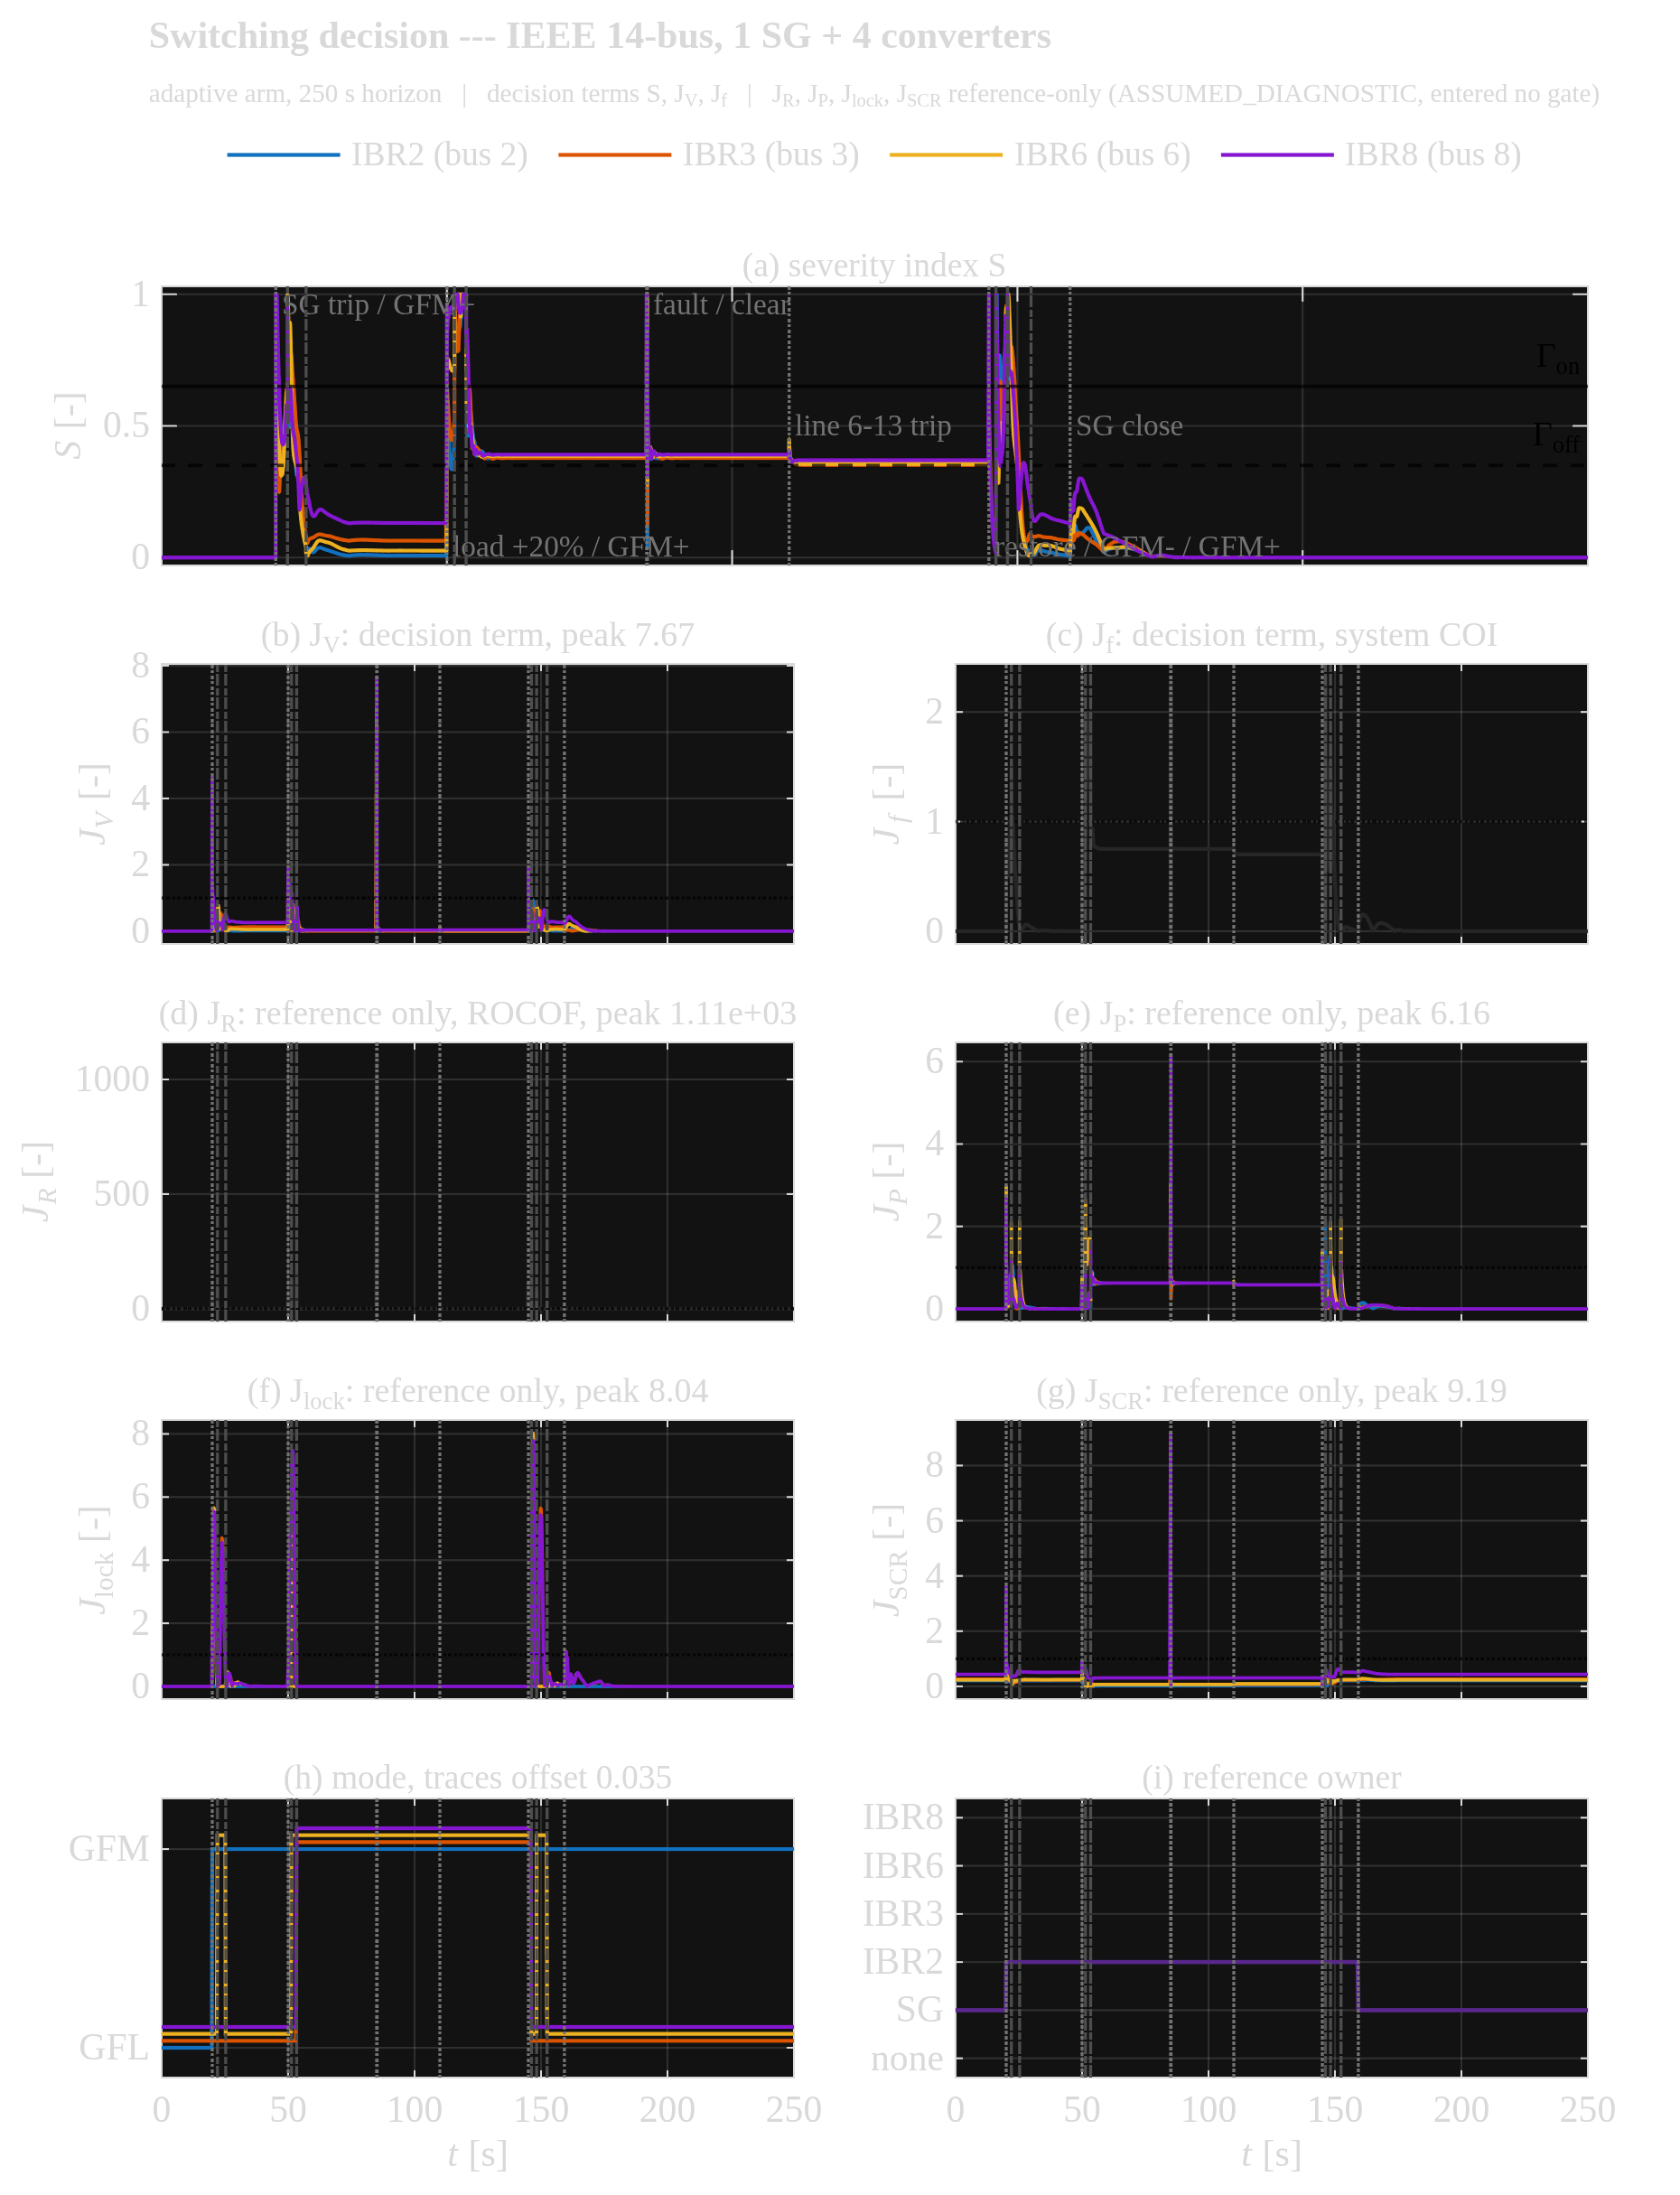
\includegraphics[width=6.20in]{figures/switch_ieee14_decision/decision_indices.png}}
 {\fbox{\parbox{6.0in}{\centering\vspace{3em}\ttfamily decision\_indices.png\\[4pt]
   \normalfont pending figure regeneration
   (run \texttt{generate\_ieee14\_switch\_evidence}).\vspace{3em}}}}
\caption{Switching-decision evidence; every panel shares one time axis and one
set of event lines. (a) Severity $S=\sat_{[0,1]}(0.5J_V+0.5J_f)$ with the
thresholds $\Gamma_{\mathrm{on}}=0.65$ and $\Gamma_{\mathrm{off}}=0.35$.
(b) $J_V$. (c) $J_f$ (system). (d) $J_R$ (system). (e) $J_P$.
(f) $J_{\mathrm{lock}}$. (g) $J_{\mathrm{SCR}}$. (h) per-device GFL/GFM mode.
(i) reference-angle owner. Dotted lines: scheduled disturbances. Dash--dotted
lines: supervisor commitments. Panels (a)--(c) decide; panels (d)--(g) are
reference-only and enter no gate.}
\label{fig:agsi}
\end{figure}

The two windows in which the switching actually happens are enlarged in
Figures~\ref{fig:agsizoom1} and~\ref{fig:agsizoom2}. In those two figures both
line families are fully labelled, so the index values at the instant of each
command can be read off directly.

\clearpage
\begin{figure}[H]
\centering
\IfFileExists{figures/switch_ieee14_decision/decision_indices_zoom_island.png}
 {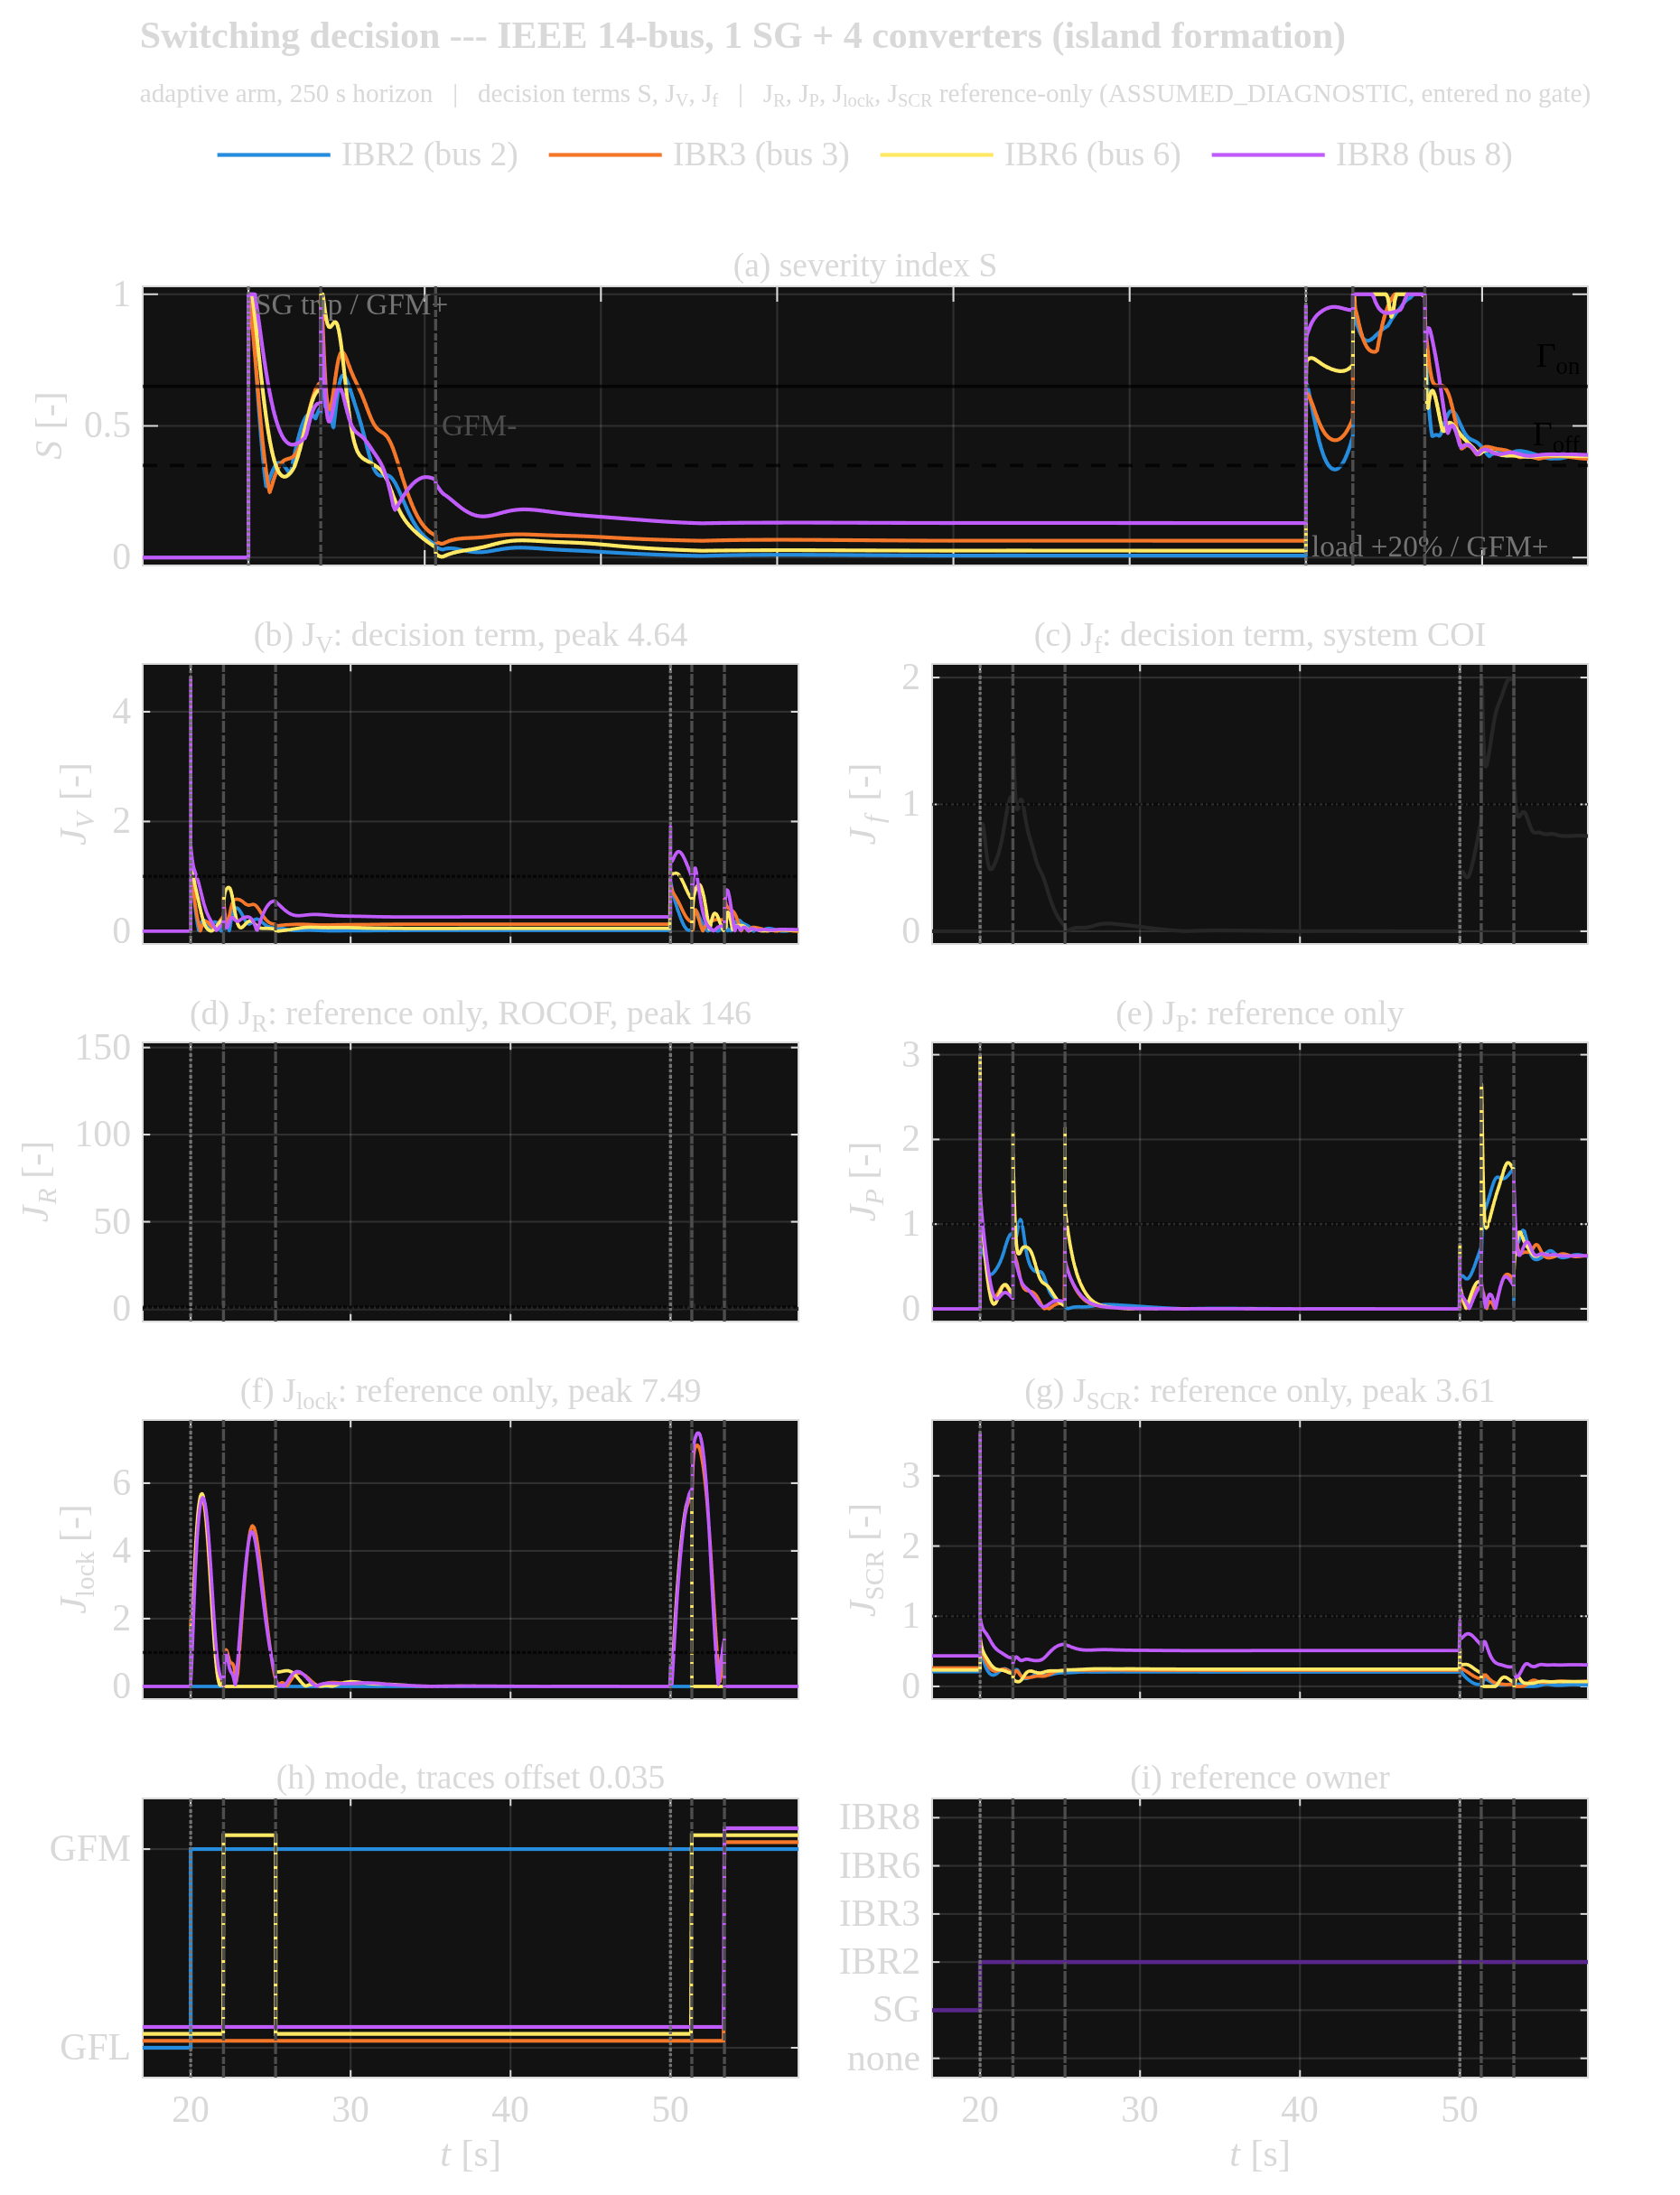
\includegraphics[width=6.20in]{figures/switch_ieee14_decision/decision_indices_zoom_island.png}}
 {\fbox{\parbox{6.0in}{\centering\vspace{3em}\ttfamily
   decision\_indices\_zoom\_island.png\\[4pt]\normalfont
   pending figure regeneration.\vspace{3em}}}}
\caption{Islanding window $t\in[17,58]\second$, covering the SG trip, the first
two mode augmentations, one release and the load step. Panels and line families
are identical to Figure~\ref{fig:agsi}; only the time range differs. No sample is
dropped or altered.}
\label{fig:agsizoom1}
\end{figure}

\clearpage
\begin{figure}[H]
\centering
\IfFileExists{figures/switch_ieee14_decision/decision_indices_zoom_reclose.png}
 {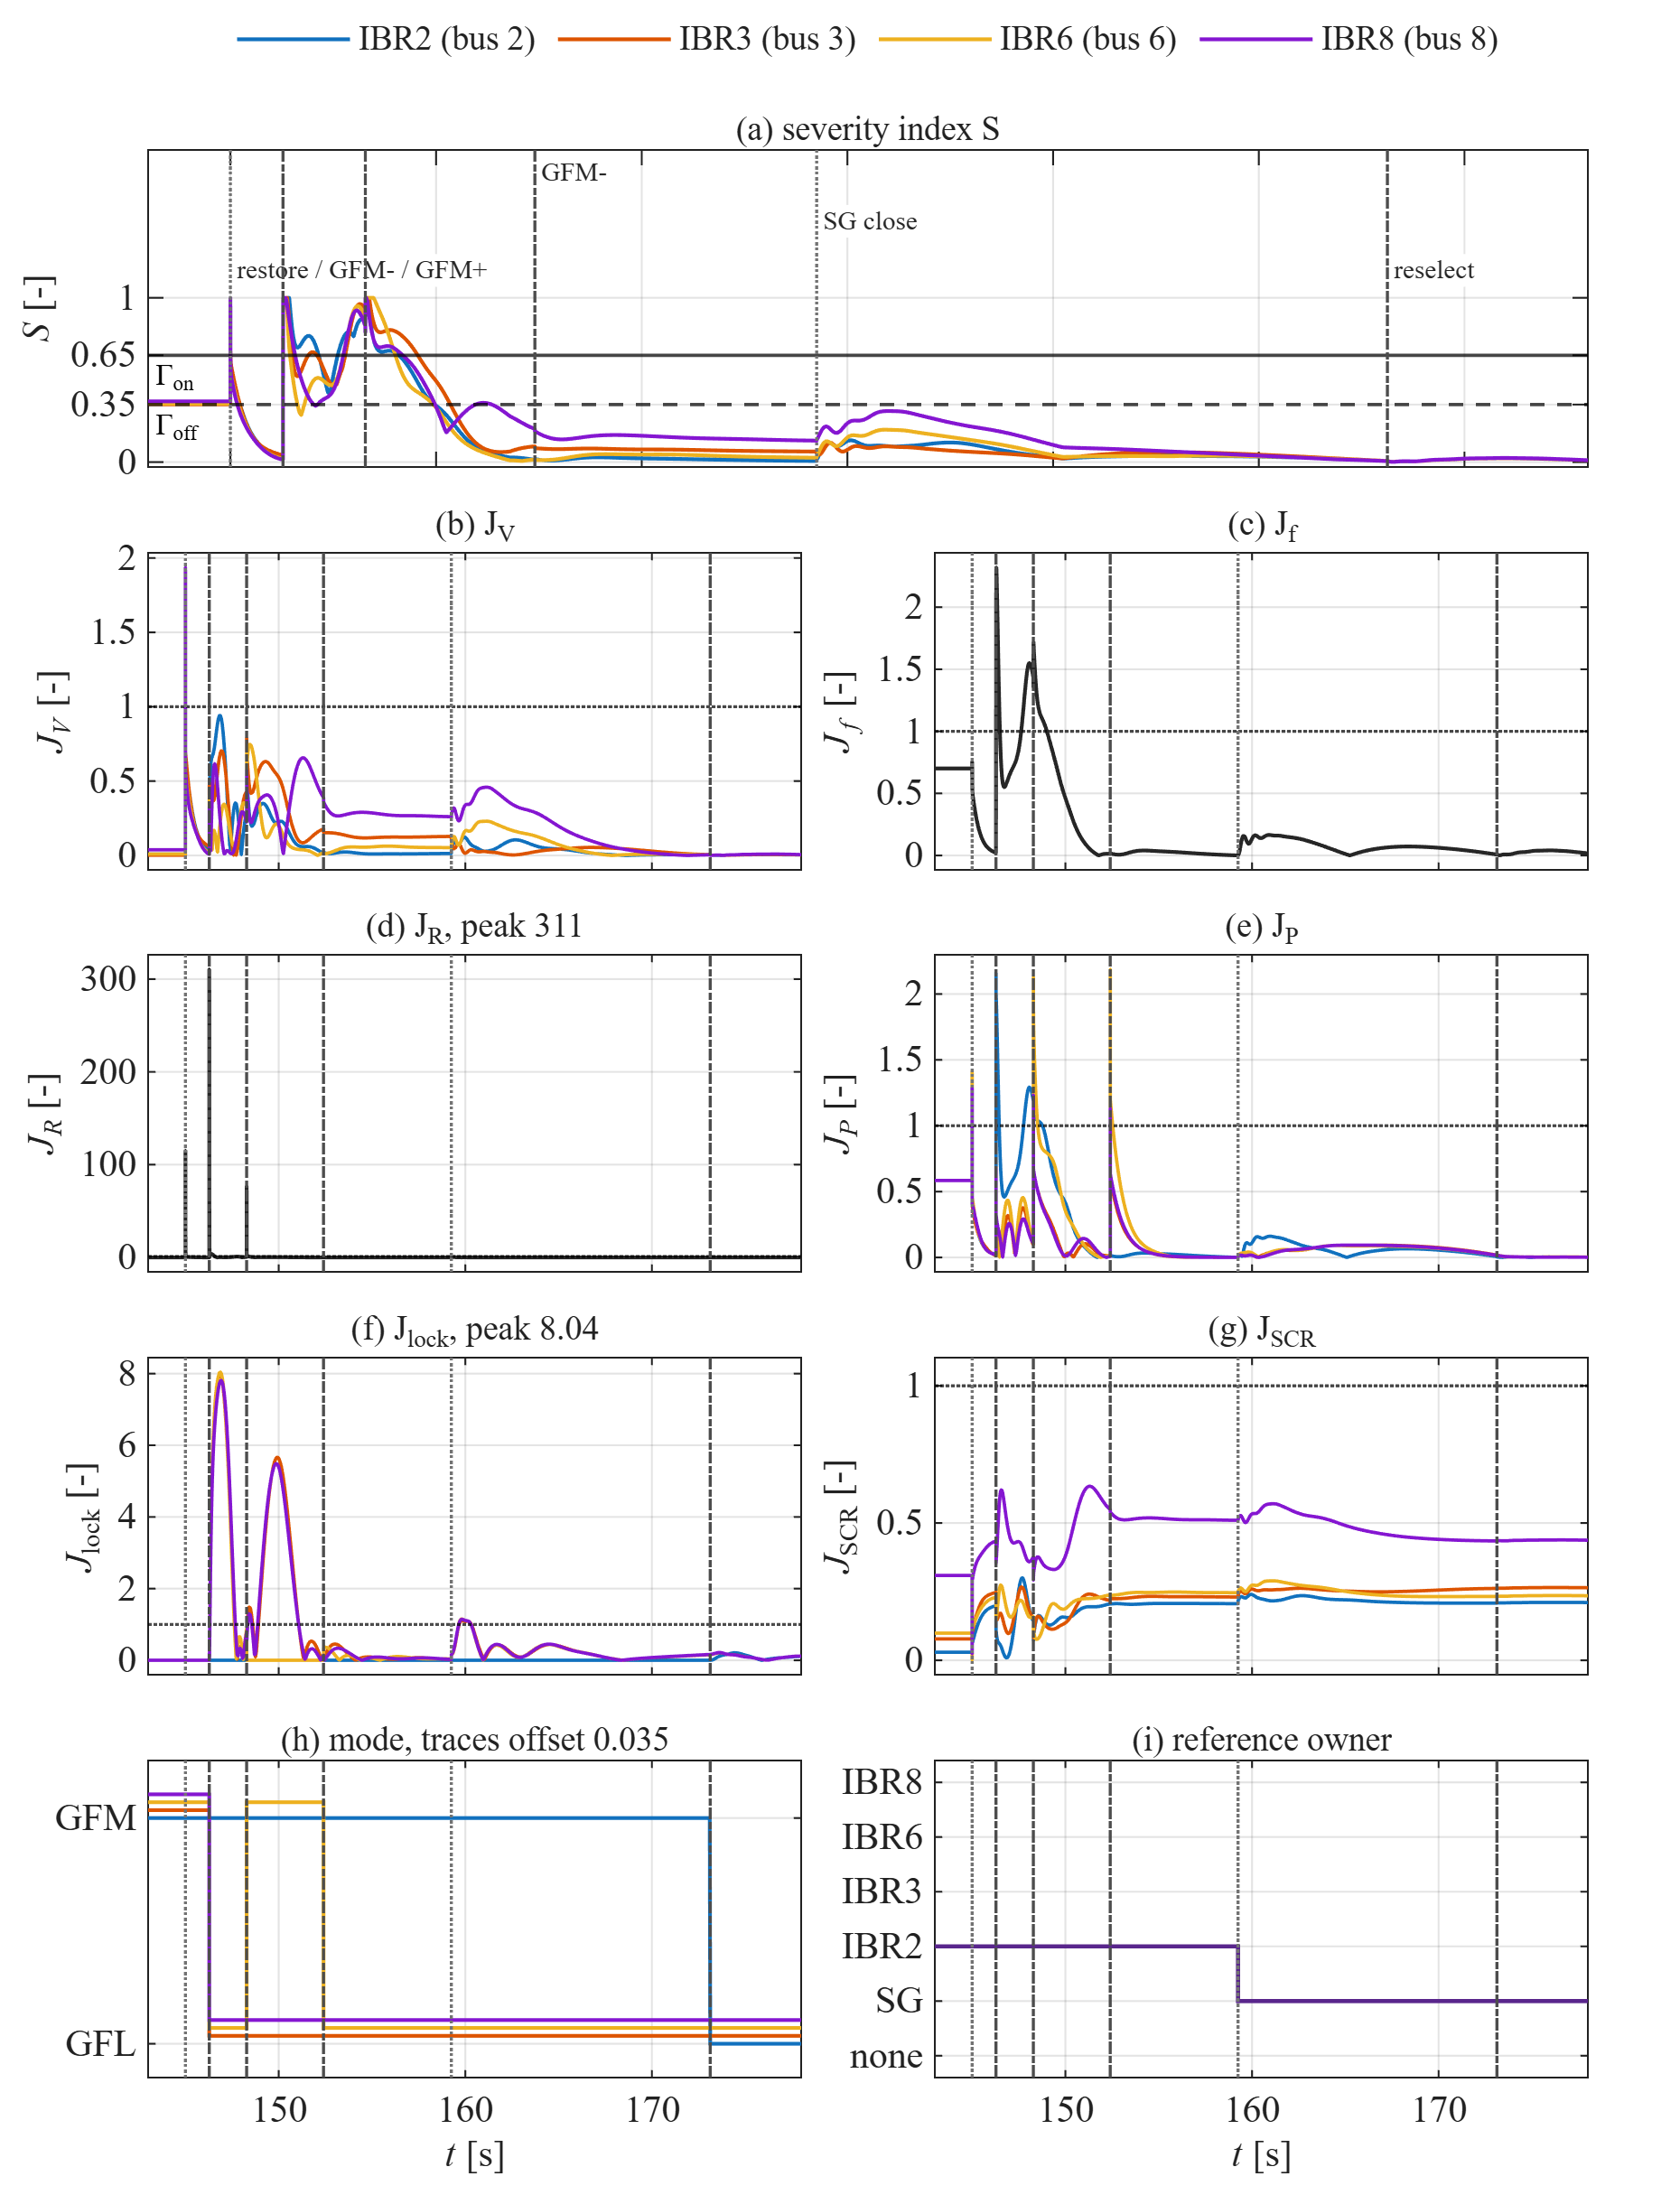
\includegraphics[width=6.20in]{figures/switch_ieee14_decision/decision_indices_zoom_reclose.png}}
 {\fbox{\parbox{6.0in}{\centering\vspace{3em}\ttfamily
   decision\_indices\_zoom\_reclose.png\\[4pt]\normalfont
   pending figure regeneration.\vspace{3em}}}}
\caption{Reclose and hand-back window $t\in[143,178]\second$, showing the mode
releases, one compensating augmentation, the reclose at
$t=\NewRunReclose\second$, and the return of reference-angle ownership to the SG.
Panels and line families are identical to Figure~\ref{fig:agsi}.}
\label{fig:agsizoom2}
\end{figure}

%=============================================================================
\section{Synchronous generator: sixth-order model and its proof}\label{sec:sg}
%=============================================================================
The SG is a sixth-order round-rotor machine of the structure IEEE~Std~1110
recommends for stability studies of this kind~\cite{ieee1110}, with state
\begin{equation}
  x_{\mathrm{sg}}=[\,\delta,\;\omega,\;E_q',\;E_d',\;E_q'',\;E_d''\,]^{\top},
  \qquad u_{\mathrm{sg}}=[\,T_m,\;E_{fd}\,]^{\top},
  \label{eq:sgstate}
\end{equation}
where $\delta$ is the rotor angle, $\omega$ the per-unit speed deviation (slip),
$E_q',E_d'$ the transient EMFs, and $E_q'',E_d''$ the subtransient EMFs. The two
control inputs $T_m$ (mechanical torque) and $E_{fd}$ (field voltage) are held at
the constant values determined by the mixed-network equilibrium solve; they are
not re-solved each step.

\paragraph{Attribution of the machine structure.}
Two lineages are easy to conflate here and are kept apart deliberately. The
\emph{structural class} --- a round-rotor machine carrying transient and
sub-transient flux pairs on both axes --- is the one IEEE~Std~1110 recommends, and
that is what the reference above supports~\cite{ieee1110}. The \emph{particular
algebraic form} in which such a machine is coded in industry tools descends from a
separate line of work on machine-model equivalence and is not an IEEE~1110 object;
the two are not interchangeable and are not treated as such here. IEEE~Std~1110
also does not itself supply the swing equation: for that it defers to the standard
textbook treatments~\cite{kundur1994,sauerpai1998}, which is the form
used in~\eqref{eq:sg1}--\eqref{eq:sg2}. No page number is quoted from the
standard, because two byte-distinct copies of it circulate and their pagination
differs; a page citation that cannot be reproduced is worse than none.

\paragraph{Where the machine numbers come from.}
The reactances, time constants and inertia of the machine at the reference bus are
\textsf{CASE\_DEFINED} values taken from the Waterloo technical report's IEEE-14
dynamic-data table~\cite{kodsi2003}, mapped onto the flux parameterisation
of~\eqref{eq:cddd}, with $H=2.5\second$ and $D=1.0\pu$ on the $100$~MVA system
base. The network topology, branch data and load schedule are the MATPOWER
distribution of the IEEE 14-bus case, itself converted from the IEEE common data
format~\cite{matpower}. Neither source is re-derived here and no value from either
is adjusted; Section~\ref{sec:pf} reports the power flow they produce.

\subsection{Order-by-order derivation}
The connected-machine equations are, term for term as coded,
\begin{align}
  \dot\delta            &= \omega_0\,\omega, \label{eq:sg1}\\
  2H\,\dot\omega        &= T_m - T_e - D\,\omega, \label{eq:sg2}\\
  T_{d0}'\,\dot{E}_q'   &= E_{fd} + c_d E_q'' - d_d E_q', \label{eq:sg3}\\
  T_{q0}'\,\dot{E}_d'   &= c_q E_d'' - d_q E_d', \label{eq:sg4}\\
  T_{d0}''\,\dot{E}_q''  &= E_q' - E_q'' - (X_d'-X_d'')\,I_d, \label{eq:sg5}\\
  T_{q0}''\,\dot{E}_d''  &= E_d' - E_d'' + (X_q'-X_q'')\,I_q, \label{eq:sg6}
\end{align}
with $\omega_0=2\pi f_0$. The air-gap electrical torque that closes the swing
equation~\eqref{eq:sg2} is
\begin{equation}
  T_e = V_d I_d + V_q I_q + R_a\,(I_d^2+I_q^2), \label{eq:sgte}
\end{equation}
and the four flux-coupling coefficients are defined from the reactance ladder as
\begin{equation}
  c_d=\frac{X_d-X_d'}{X_d'-X_d''},\quad
  d_d=\frac{X_d-X_d''}{X_d'-X_d''},\quad
  c_q=\frac{X_q-X_q'}{X_q'-X_q''},\quad
  d_q=\frac{X_q-X_q''}{X_q'-X_q''}.
  \label{eq:cddd}
\end{equation}

\emph{What each order is.}
Equations~\eqref{eq:sg1}--\eqref{eq:sg2} are the mechanical (2nd-order) swing:
angle and speed. Equations~\eqref{eq:sg3}--\eqref{eq:sg4} are the transient (rotor
field / q-axis damper) fluxes on the slow time constants $T_{d0}',T_{q0}'$.
Equations~\eqref{eq:sg5}--\eqref{eq:sg6} are the subtransient (damper) fluxes on
the fast time constants $T_{d0}'',T_{q0}''$. The armature-reaction terms
$-(X_d'-X_d'')I_d$ and $+(X_q'-X_q'')I_q$ couple the fast fluxes to the stator
current.

\emph{Proof anchor --- the $d-c=1$ identity.}
From~\eqref{eq:cddd},
\begin{equation}
  d_d-c_d=\frac{(X_d-X_d'')-(X_d-X_d')}{X_d'-X_d''}
         =\frac{X_d'-X_d''}{X_d'-X_d''}=1,
  \qquad\text{and identically } d_q-c_q=1.
  \label{eq:identity}
\end{equation}
Consider the open-circuit steady state ($I_d=I_q=0$, $\dot x=0$). Then
\eqref{eq:sg5} gives $E_q''=E_q'$, and substituting into~\eqref{eq:sg3},
\begin{equation}
  0=E_{fd}+c_d E_q'-d_d E_q'=E_{fd}-(d_d-c_d)E_q'=E_{fd}-E_q'
  \;\Longrightarrow\; E_q'=E_{fd}.
\end{equation}
So the identity~\eqref{eq:identity} is exactly what makes the open-circuit field
EMF equal the applied field voltage --- the standard consistency check for this
flux parameterisation, and the reason the coefficients are written as
ratios~\eqref{eq:cddd} rather than as free constants. The same argument on the
q-axis gives $E_d'=0$ at open circuit when $E_{fd}$ has no q-axis analogue.

\subsection{Algebraic stator interface}
The stator currents are \emph{not} reverse-derived from power; they are solved
from the subtransient EMFs behind subtransient reactance. Projecting the complex
terminal voltage $V$ onto the machine $dq$ frame ($V_d,V_q$) and writing
$r_d=V_d-E_d''$, $r_q=V_q-E_q''$,
\begin{equation}
  \det=X_d''X_q''+R_a^2,\qquad
  I_d=\frac{-R_a r_d - X_q'' r_q}{\det},\qquad
  I_q=\frac{X_d'' r_d - R_a r_q}{\det},
  \label{eq:stator}
\end{equation}
which is the exact inverse of the subtransient stator relations
$V_d=E_d''-R_a I_d+X_q'' I_q$, $V_q=E_q''-R_a I_q-X_d'' I_d$. The electrical
torque~\eqref{eq:sgte} uses these same $I_d,I_q$.

\subsection{The singular limit that freezes $E_d'$}\label{sec:frozen}
For the machine data used here the q-axis transient open-circuit time constant is
set to its singular limit $T_{q0}'=0$ (audited round-rotor case). Then
\eqref{eq:sg4} is no longer differential: it degenerates to the algebraic
constraint
\begin{equation}
  0 = c_q E_d'' - d_q E_d'.
\end{equation}
For this machine $c_q=0,\;d_q=1$, so $E_d'\equiv 0$. The code detects
$T_{q0}'=0$ exactly and \emph{removes} $E_d'$ (state index~4) from the integrated
set, holding it at its algebraic value $0$. The SG therefore contributes
\textbf{five} dynamic states $[\delta,\omega,E_q',E_q'',E_d'']$, not six. This is
a \textsf{SOURCE\_DEFINED} singular limit, not a numerical convenience: it is the
$T_{q0}'\to0$ reduction of the same equations.

\subsection{Breaker-open coast}
When the SG breaker opens at $t=20$~s the machine does not vanish from the state
vector. Its network injection becomes zero ($I_d=I_q=0$, $T_e=0$) and its fluxes
decay on the open-circuit branch of~\eqref{eq:sg3}--\eqref{eq:sg6} (the
armature-reaction terms drop out because $I_d=I_q=0$); the swing
\eqref{eq:sg1}--\eqref{eq:sg2} coasts on a frozen mechanical torque $T_m$. The
map that reports how many states the SG integrates is context-independent: it
returns $[\,1,2,3,5,6\,]$ whether the breaker is closed or open. Consequently the
loss of the SG slack does \emph{not} change the SG's own state count; the
composite dimension changes only because the IBRs switch mode
(Section~\ref{sec:ibr}).

%=============================================================================
\section{Inverter-based resource: the dual-mode 16-state model}\label{sec:ibr}
%=============================================================================
Each IBR is a single device that can present either of two controllers on a
common power stage. The full state is a fixed 16-vector,
\begin{equation}
  x_{\mathrm{IBR}}
   =\bigl[\underbrace{i_d,\,i_q,\,V_{dc}}_{\substack{x_{\mathrm{pl}}\;(3)\\
            \text{\scriptsize always live}}}\;\big|\;
          \underbrace{x_{\mathrm{GFL}}\;(6)}_{\substack{\text{indices }4\text{--}9\\
            \text{\scriptsize live only in GFL}}}\;\big|\;
          \underbrace{x_{\mathrm{GFM}}\;(7)}_{\substack{\text{indices }10\text{--}16\\
            \text{\scriptsize live only in GFM}}}\bigr]^{\top}
   \in\mathbb{R}^{16}.
   \label{eq:ibrstate}
\end{equation}

\paragraph{The two controllers never run at the same time.}
Equation~\eqref{eq:ibrstate} is a fixed \emph{superset} of coordinates, not a
list of simultaneously live states, and this is the single most important thing
to read correctly about the device. A converter is \emph{either} grid-following
\emph{or} grid-forming at any instant, never both and never partly each: one
controller block is integrated while the other is held frozen at the value it
carried when it last surrendered the duty, and the two can exchange the duty
only at a switching instant, through the transfer of
Section~\ref{sec:transfer}. There is no blend, no weighted average of the two
control laws, and no interval on which both sets of integrators advance. The
consequence for any later reading of the state vector is concrete: an index in
the frozen block is not a measurement of anything during that interval, so a
quantity built from a fixed index across a mode change is not a physical
signal.

The shorthand $x_{\mathrm{IBR}}=[x_{\mathrm{GFM}}\;x_{\mathrm{GFL}}]$ is the
same object with the shared plant block $x_{\mathrm{pl}}$ made explicit and the
two controller blocks kept in their code order. The controller blocks are
\begin{align}
  x_{\mathrm{GFL}}&=[\,\delta_{\mathrm{PLL}},\,\xi_{\mathrm{PLL}},\,\xi_P,\,\xi_Q,
      \,\xi_{Id},\,\xi_{Iq}\,],\\
  x_{\mathrm{GFM}}&=[\,\delta_{\mathrm{VSG}},\,\omega_{\mathrm{VSG}},\,E,
      \,\xi_{Vd},\,\xi_{Vq},\,\xi_{Id},\,\xi_{Iq}\,].
\end{align}
Only a projection of~\eqref{eq:ibrstate} is integrated at any instant. The
active-index map returns
\begin{equation}
  \mathcal{A}_{\mathrm{GFL}}=\{1{:}9\},\qquad
  \mathcal{A}_{\mathrm{GFM}}=\{1{:}3,\,10{:}16\},\qquad
  \mathcal{A}_{\mathrm{tripped}}=\varnothing,
  \label{eq:ibractive}
\end{equation}
i.e.\ 9 active states in GFL, 10 in GFM, none when tripped. The intersection
$\mathcal{A}_{\mathrm{GFL}}\cap\mathcal{A}_{\mathrm{GFM}}=\{1,2,3\}$ is exactly
the shared plant, and the union is all of $\{1{:}16\}$: the plant is always
live, and every controller index belongs to one branch alone. The active count
is therefore $9$ or $10$, never $16$ --- the superset dimension is never the
dynamic dimension. With
one SG contributing six stored states, the composite state vector of this study
therefore has $6+4\times16=70$ rows, which is exactly the row count of the stored
trajectory.

\subsection{Reduced command-delay states}\label{sec:ibr-reduction}
The source block diagram carries one first-order actuation lag per axis,
$T_d\,\dot V_{\mathrm{del}}=v_{\mathrm{cmd}}-V_{\mathrm{del}}$, whose physical
time constant is the digital-converter delay
$T_d=1.5/f_{\mathrm{sw}}\approx0.3$~ms at $f_{\mathrm{sw}}=5$~kHz. That is more
than two orders of magnitude below the phasor step used here, so by singular
perturbation the fast lag collapses onto its slow manifold
$V_{\mathrm{del}}=v_{\mathrm{cmd}}$: the two delay states per branch are removed
algebraically and the filter-current equations use the commanded voltage
$v_{cd},v_{cq}$ directly. This is a standard model-order reduction that leaves
both the equilibrium and the retained-state dynamics unchanged, and it removes a
pole near $530$~Hz that an RMS phasor network model cannot represent in the first
place. The reduction takes the dual-mode superset from $20$ to the $16$ states
of~\eqref{eq:ibrstate} and each standalone branch from $12$ to $10$. It is
\textsf{PROJECT\_DERIVED} and owner-set; see defect record
\textsf{TD-2026-08-12-01}. Report revisions before this one printed the
pre-reduction $20$-state layout, which the executed model no longer has.

Two operators recur below; their structural role in a limited converter is the
standard one~\cite{bacha2014}, while the particular directional anti-windup
realisation is \textsf{PROJECT\_DERIVED}. $\Pi_I(a,b;I_{\max})$ is the
\emph{circular} current
limiter: if $r=\sqrt{a^2+b^2}>I_{\max}$ it scales $(a,b)\mapsto(a,b)\,I_{\max}/r$,
else it is the identity; its rejected part is the limiter residual
$r_i=(a,b)-\Pi_I(a,b)$. $\mathcal{H}(e,\gamma,r_i,\text{sat})$ is the conditional
anti-windup integrator: it returns $0$ when the reference is clipped and the
error would wind further ($\text{sat}$ and $\gamma\,e\,r_i>0$), and $e$ otherwise.
The instantaneous injection is $I=(i_d+\mathrm{j}i_q)e^{\mathrm{j}\theta}/\kappa$,
$S=V\overline{I}$, $P_{\mathrm{inv}}=\kappa\Re S$, $Q_{\mathrm{inv}}=\kappa\Im S$,
with $\kappa=S_{\mathrm{base}}/M_{\mathrm{base}}$ and $(v_d,v_q)=\Re,\Im\,(Ve^{-\mathrm{j}\theta})$.

\subsection{Shared power stage (states 1--3)}
The $L$-filter current dynamics and DC-link are common to both modes and are
always active. Written one state per line in index order:
\begin{align}
  \tfrac{L}{\omega_b}\,\dot{i}_d &= v_{cd}-v_d-R\,i_d+\omega L\,i_q,
    &&\text{ $d$-axis filter current}\\
  \tfrac{L}{\omega_b}\,\dot{i}_q &= v_{cq}-v_q-R\,i_q-\omega L\,i_d,
    &&\text{ $q$-axis filter current}\\
  \dot{V}_{dc} &= \tfrac{1}{C}\!\left[\tfrac{E_{dc}-V_{dc}}{R_{dc}}
      -\frac{P_{ac}}{V_{dc}}
      -\frac{\max(0,\,V_{dc}-V_{dc}^{\max})}{R_{ch}}\right],
    &&\text{ DC-link voltage}
\end{align}
with $R=R_f$, $L=L_f$, $C=C_{dc}$, $\omega_b=2\pi f_b$, and $v_{cd},v_{cq}$ the
inner-loop commanded voltages defined per branch below. The DC-link row is
derived in Section~\ref{sec:dcsource}; $P_{ac}=v_{cd}i_d+v_{cq}i_q$ there is the
converter-side power, that is the bus power plus the filter loss, which is what
the DC bus actually has to supply. The commanded voltage
appears here rather than a delayed command because of the reduction of
Section~\ref{sec:ibr-reduction}. \emph{Proof of each row.}
Rows (1)--(2) are Kirchhoff's voltage law across the series $R_f,L_f$ filter in
the rotating frame; the cross terms $\pm\omega L$ are the frame-rotation EMF, and
the rotation rate $\omega$ is supplied by whichever controller is active (the PLL
in GFL, the VSG swing in GFM) --- this is the only place the plant equations feel
the mode. Row (3) is the \textsf{PROJECT\_DERIVED} DC-source closure: the coded
current is $I_{dc}=P_{ac}/V_{dc}+(C/T_{dc})(V_{dc}^{0}-V_{dc})$ and
$\dot V_{dc}=(I_{dc}-P_{ac}/V_{dc})/C$, in which the power feed-forward
$P_{ac}/V_{dc}$ cancels exactly, leaving the first-order voltage restoration
shown. This cancellation is deliberate: the unpublished DC source cannot move the
sourced AC equilibrium. At steady state row (3) gives $V_{dc}=V_{dc}^{0}$.

\subsection{Non-ideal DC source}\label{sec:dcsource}
The source publishes the DC-link energy balance
$C\dot V_{dc}=I_{dc}-P_{ac}/V_{dc}$ but not the law for $I_{dc}$, so the law is
\textsf{PROJECT\_DERIVED} and has to be stated and justified rather than
assumed. Any DC-side source --- a rectifier, a battery, a photovoltaic string in
its voltage-source region, or a DC feeder --- is to first order an EMF behind its
internal plus cable resistance, which gives
\begin{equation}
  I_{dc}=\frac{E_{dc}-V_{dc}}{R_{dc}},
  \label{eq:dcsrc}
\end{equation}
and, with the overvoltage chopper of~\eqref{eq:dcchop} below, the DC-link row
of the shared power stage.

\paragraph{$E_{dc}$ is forced, not chosen.} Requiring the dispatched point to be
an equilibrium, $\dot V_{dc}=0$ at $V_{dc}=V_{dc}^{0}$ and $P_{ac}=P_{ac}^{0}$,
leaves exactly one admissible value,
\begin{equation}
  E_{dc}=V_{dc}^{0}+\frac{R_{dc}P_{ac}^{0}}{V_{dc}^{0}},\qquad
  P_{ac}^{0}=\kappa P_{\mathrm{ref}}+R_f\bigl(i_{d0}^{2}+i_{q0}^{2}\bigr),
  \label{eq:dcedc}
\end{equation}
in closed form, because at the initial point both branches set
$i_{d0}=\kappa P_{\mathrm{ref}}/|V_0|$ and $i_{q0}=-\kappa Q_{\mathrm{ref}}/|V_0|$
with $\theta=\angle V_0$, so $v_d=|V_0|$, $v_q=0$, and the two $\omega L$ cross
terms of $v_{cd}i_d+v_{cq}i_q$ cancel identically. Two consequences matter.
First, the sourced AC initial condition and therefore the power flow of
Section~\ref{sec:pf} are untouched: the measured $\dot V_{dc}(0)$ is zero to
round-off. Second, because~\eqref{eq:dcedc} is evaluated from the same
$P_{\mathrm{ref}},Q_{\mathrm{ref}},V_0,R_f$ in both branches, $E_{dc}$ is
identical in GFL and GFM, so a run-time transfer introduces no step in
$\dot V_{dc}$ and not merely none in $V_{dc}$.

\paragraph{$R_{dc}$ from a declared regulation, bounded by a reachability
requirement.} Let $\varepsilon$ be the DC-source regulation, the fractional DC
voltage rise from the dispatched point to no load at rated converter power
$P_r$, so that $R_{dc}=\varepsilon (V_{dc}^{0})^{2}/P_r$. The equilibrium
of~\eqref{eq:dcsrc} against a constant-power draw $P$ satisfies
$V_{dc}^{2}-E_{dc}V_{dc}+R_{dc}P=0$, which has a real solution only while
\begin{equation}
  E_{dc}^{2}\ \ge\ 4R_{dc}P_{\max},\qquad P_{\max}=V_{\max}I_{\max},
  \label{eq:dcdisc}
\end{equation}
so requiring margin $m$ in~\eqref{eq:dcdisc} bounds $\varepsilon$ from above. At
$m=2$ with $V_{\max}=1.06\pu$, $I_{\max}=1.2\pu$ and the dispatched
$P_{\mathrm{ref}}$ of this study the bound is $\varepsilon\lesssim0.115$. The
declared value is $\varepsilon=0.10$, which sits inside that bound with realised
margin $2.15$ and coincides with the usual ten per cent regulation of a DC link
fed through a boost stage or a feeder. It is \emph{not} chosen to suit the
integrator step; see the stiffness statement below.

\paragraph{The link cannot run away, and this is proved rather than assumed.}
For $V_{dc}>E_{dc}$ every term of the DC-link row is negative whenever
$P_{ac}\ge0$, hence $\dot V_{dc}<0$ and
\begin{equation}
  V_{dc}(t)\ \le\ \max\bigl(V_{dc}(0),E_{dc}\bigr)=E_{dc}
   =V_{dc}^{0}\Bigl(1+\varepsilon P_{ac}^{0}/(V_{dc}^{0})^{2}\Bigr)
  \quad\text{for all }t.
  \label{eq:dcbound}
\end{equation}
When the network collapses during a fault and $P_{ac}\to0$, the link therefore
rises only towards $E_{dc}$; the internal resistance is itself the limit. The
overvoltage chopper is a braking resistor conducting in its linear region,
\begin{equation}
  I_{ch}=\frac{\max\bigl(0,\,V_{dc}-V_{dc}^{\max}\bigr)}{R_{ch}},
  \label{eq:dcchop}
\end{equation}
continuous and Lipschitz, non-differentiable only on $V_{dc}=V_{dc}^{\max}$ in
exactly the way $\Pi_I$ is, so it needs no separate smoothness argument and is
covered by Remark~\ref{rem:nonsmooth}. By~\eqref{eq:dcbound} it is inactive
whenever $E_{dc}\le V_{dc}^{\max}$, which holds here; it is retained because a
real converter has one and a different dispatch would engage it, and whether it
conducted on a given trajectory is decided afterwards from $\max_t V_{dc}$
against $V_{dc}^{\max}$, which is exact because the conduction condition depends
on $V_{dc}$ alone.

\paragraph{The stiffness this exposes is reported, not designed around.}
Linearising the DC-link row with the chopper off about the dispatched point gives
\begin{equation}
  \lambda_{dc}=-\frac{1}{C}\left(\frac{1}{R_{dc}}-\frac{P_{ac}^{0}}{(V_{dc}^{0})^{2}}\right),
  \label{eq:dclam}
\end{equation}
whose second term is the negative incremental resistance of a constant-power
load, so stability requires $R_{dc}<(V_{dc}^{0})^{2}/P_{ac}^{0}$ --- a condition
this configuration satisfies by a wide factor. With $C=C_{dc}=0.10$ and
$R_{dc}=0.10$ the mode is near $-95\ \mathrm{s^{-1}}$, a time constant of about
$10$~ms, so $|\lambda_{dc}|\,\Delta t\approx4.8$ at the nominal phasor step
$\Delta t=0.05\second$. The implicit trapezoidal rule is A-stable there, but the
mode is under-resolved at the nominal step and the adaptive controller has to
reduce $\Delta t$ where it is excited. $\varepsilon$ was deliberately not
enlarged to bring $|\lambda_{dc}|\Delta t$ near unity: choosing a physical
parameter to suit a step size is reverse-engineering it from numerical
convenience. The honest consequence is the reverse of a convenience --- a
\emph{firmer} DC source, $\varepsilon$ of order $0.01$ for a battery at the
terminals, is stiffer still and belongs to an EMT study rather than to a
$50$~ms phasor step. That is a limit of this class of simulation, stated here
rather than hidden by an idealisation.

\paragraph{What this replaced, and why.} Revisions of this report before the
present one carried a closure with an exact instantaneous power feed-forward,
$I_{dc}=P_{ac}/V_{dc}+(C/T_{dc})(V_{dc}^{0}-V_{dc})$, which cancels the AC
loading identically and collapses the link to
$\dot V_{dc}=(V_{dc}^{0}-V_{dc})/T_{dc}$. Two measured consequences identify it
as an ideal DC source. Its own initial condition $V_{dc}(0)=V_{dc}^{0}$ is the
equilibrium of that scalar equation, so $V_{dc}$ stayed at $1.000000000000\pu$
for every accepted sample of every converter over the whole $250\second$ run,
range exactly zero --- the coordinate carried no information. And because $C$
cancels, the declared capacitance $C_{dc}$ never entered any residual. Both are
removed by~\eqref{eq:dcsrc}--\eqref{eq:dcchop}, in which $C_{dc}$ appears for the
first time in~\eqref{eq:dclam} and $V_{dc}$ is a live coordinate driven by
$P_{ac}$.

\subsection{GFL (states 4--9)}
The auxiliary algebraic quantities are the power errors
$e_P=\kappa u_1-P_{\mathrm{inv}}$, $e_Q=\kappa u_2-Q_{\mathrm{inv}}$, the raw and
clipped current references
\begin{equation}
  i_{d,\mathrm{ref}}^{\mathrm{raw}}=k_{pP}e_P+k_{iP}\xi_P,\quad
  i_{q,\mathrm{ref}}^{\mathrm{raw}}=-(k_{pQ}e_Q+k_{iQ}\xi_Q),\quad
  [i_{d,\mathrm{ref}},i_{q,\mathrm{ref}}]=\Pi_I(\cdot;I_{\max}),
\end{equation}
and the inner voltage commands
$v_{cd}=v_d+R i_d-\omega L i_q+k_{pI}(i_{d,\mathrm{ref}}-i_d)+k_{iI}\xi_{Id}$,
$v_{cq}=v_q+R i_q+\omega L i_d+k_{pI}(i_{q,\mathrm{ref}}-i_q)+k_{iI}\xi_{Iq}$.
The six GFL states then evolve, one per line in index order:
\begin{align}
  \dot{\delta}_{\mathrm{PLL}} &= k_{p,\mathrm{PLL}}v_q+k_{i,\mathrm{PLL}}\xi_{\mathrm{PLL}},
     &&\text{ PLL angle};\quad \omega=1+\dot\delta_{\mathrm{PLL}}/\omega_b\\
  \dot{\xi}_{\mathrm{PLL}} &= v_q, &&\text{ PLL integrator}\\
  \dot{\xi}_P &= \mathcal{H}(e_P,\,k_{iP},\,r_{i,d},\,\text{sat}),
     &&\text{ active-power integrator}\\
  \dot{\xi}_Q &= \mathcal{H}(e_Q,\,-k_{iQ},\,r_{i,q},\,\text{sat}),
     &&\text{ reactive-power integrator}\\
  \dot{\xi}_{Id} &= i_{d,\mathrm{ref}}-i_d, &&\text{ $d$-current integrator}\\
  \dot{\xi}_{Iq} &= i_{q,\mathrm{ref}}-i_q, &&\text{ $q$-current integrator}
\end{align}
\emph{Proof of each state.} (4)--(5) are the synchronous-reference-frame PLL: it
drives the measured $q$-axis voltage $v_q$ to zero, so at lock $\dot\xi_{\mathrm{PLL}}
=v_q=0$ and the frame is aligned with the terminal voltage; the loop frequency is
$\omega=1+\dot\delta_{\mathrm{PLL}}/\omega_b$. (6)--(7) are the outer $P$/$Q$ PIs:
at equilibrium $\dot\xi_P=e_P=0$ forces $P_{\mathrm{inv}}=\kappa u_1$ and
$\dot\xi_Q=e_Q=0$ forces $Q_{\mathrm{inv}}=\kappa u_2$, i.e.\ the IBR meets its
$P,Q$ set-points; the $\mathcal H$ wrapper freezes them only while the current
reference is on the $I_{\max}$ circle. (8)--(9) are the inner current PIs:
$\dot\xi_{Id}=i_{d,\mathrm{ref}}-i_d=0$ makes the filter current track its
reference (and symmetrically on $q$). The two command-lag states that the source
diagram places between $v_{cd},v_{cq}$ and the filter are not integrated here;
they are on their slow manifold by Section~\ref{sec:ibr-reduction}, so
$V_{d,\mathrm{del}}=v_{cd}$ and $V_{q,\mathrm{del}}=v_{cq}$ identically --- which
is the same steady-state relation the lag would have given, reached without
carrying an unresolvable fast pole. The GFL branch is a \emph{current source}: it
needs the PLL to know the grid angle, so it cannot by itself define a voltage on a
dead network.

\subsection{GFM (states 10--16): voltage source, VSG}
The grid-forming branch replaces the PLL by a virtual-synchronous-generator swing
and a $Q$--$V$ voltage-forming loop. The voltage references are
$v_{d,\mathrm{ref}}=E$, $v_{q,\mathrm{ref}}=0$; the voltage errors are
$e_{vd}=E-v_d$, $e_{vq}=-v_q$; the raw/clipped current references are
$i_{d,\mathrm{ref}}^{\mathrm{raw}}=k_{pV}e_{vd}+k_{iV}\xi_{Vd}$,
$i_{q,\mathrm{ref}}^{\mathrm{raw}}=k_{pV}e_{vq}+k_{iV}\xi_{Vq}$,
$[i_{d,\mathrm{ref}},i_{q,\mathrm{ref}}]=\Pi_I(\cdot;I_{\max})$; and the inner
commands $v_{cd},v_{cq}$ are as in the GFL branch but with $\omega\to\omega_{\mathrm{VSG}}$.
The seven GFM states evolve, one per line in index order:
\begin{align}
  \dot{\delta}_{\mathrm{VSG}} &= \omega_b(\omega_{\mathrm{VSG}}-1), &&\text{ VSG angle}\\
  M\,\dot{\omega}_{\mathrm{VSG}} &= \kappa u_1-P_{\mathrm{inv}}-D_v(\omega_{\mathrm{VSG}}-1),
     &&\text{ VSG swing}\\
  \tau_E\,\dot{E} &= k_Q(\kappa u_2-Q_{\mathrm{inv}})-k_E(E-E_{\mathrm{ref}}),
     &&\text{ $Q$--$V$ voltage state}\\
  \dot{\xi}_{Vd} &= \mathcal{H}(e_{vd},\,k_{iV},\,r_{i,d},\,\text{sat}),
     &&\text{ $d$-voltage integrator}\\
  \dot{\xi}_{Vq} &= \mathcal{H}(e_{vq},\,k_{iV},\,r_{i,q},\,\text{sat}),
     &&\text{ $q$-voltage integrator}\\
  \dot{\xi}_{Id} &= i_{d,\mathrm{ref}}-i_d, &&\text{ $d$-current integrator}\\
  \dot{\xi}_{Iq} &= i_{q,\mathrm{ref}}-i_q, &&\text{ $q$-current integrator}
\end{align}
\emph{Proof of each state.} (10)--(11) are the VSG: the swing gives the converter
its \emph{own} angle from active-power balance, $M\dot\omega_{\mathrm{VSG}}
=\kappa u_1-P_{\mathrm{inv}}-D_v(\omega_{\mathrm{VSG}}-1)$, so at equilibrium
$\omega_{\mathrm{VSG}}=1$ and $P_{\mathrm{inv}}=\kappa u_1$; because the angle is
generated internally there is \emph{no PLL} and the branch can energise a passive
network. (12) is the $Q$--$V$ loop whose state $E$ \emph{is} the voltage-loop
reference $v_{d,\mathrm{ref}}=E$: at equilibrium $E=E_{\mathrm{ref}}
+(k_Q/k_E)(\kappa u_2-Q_{\mathrm{inv}})$, a droop between reactive set-point and
formed voltage. (13)--(14) are the voltage PIs that drive $v_d\to E$, $v_q\to 0$
(so the terminal voltage aligns with the VSG angle at magnitude $E$); (15)--(16)
the inner current PIs. As in the GFL branch the two command lags are on their slow
manifold and are not integrated (Section~\ref{sec:ibr-reduction}). The
anti-windup $\mathcal H$ again holds the voltage integrators only while the
current reference is saturated. The GFM branch is a \emph{voltage source}: this is
why at least one grid-forming converter must exist for the island to have a
reference angle at all.

\subsection{Current-continuity-gated transfer}\label{sec:transfer}
When the supervisor changes an IBR's mode, the new-mode controller states are not
continued by integration; they are \emph{re-initialised} at the current terminal
operating point so that the injected current does not jump. Let the pre-switch
state $x^{-}$ inject $I^{-}=I(x^{-},V)$ with $S=V\overline{I^{-}}$,
$P=\Re S$, $Q=\Im S$. The transfer $x^{-}\mapsto x^{+}$ is
\begin{equation}
  x^{+}_{\mathrm{pl}}=x^{-}_{\mathrm{pl}}\ (\text{carry }i_d,i_q,V_{dc}),\qquad
  x^{+}_{\mathrm{ctrl}}=\text{equilibrium\_initialize}(V,P,Q),
  \label{eq:transfer}
\end{equation}
with one physical carry-across of frequency: GFL$\to$GFM sets
$\omega_{\mathrm{VSG}}\!:=\!\omega_{\mathrm{PLL}}$, and GFM$\to$GFL sets the PLL
integrator $\xi_{\mathrm{PLL}}\!:=\!\omega_b(\omega_{\mathrm{VSG}}-1)/k_{i,\mathrm{PLL}}$.
The transfer is then \emph{gated}: the post-switch injection $I^{+}=I(x^{+},V)$
must satisfy
\begin{equation}
  \bigl|I^{+}-I^{-}\bigr|\le\varepsilon_{\mathrm{tol}}=10^{-10},
  \label{eq:contgate}
\end{equation}
otherwise the step is rejected fail-closed. Equation~\eqref{eq:contgate} is the
bumpless-transfer guarantee: the mode may change discontinuously in
\emph{parameterisation}, but the current the network sees is continuous.

%=============================================================================
\section{Switched time-domain formulation}\label{sec:ts}
%=============================================================================
The composite system is advanced in time by \emph{one} coupled implicit step
that the plain and the hybrid drivers share. Three questions are answered in
turn, because they are the three things that make this harder than integrating a
single machine: (i)~the differential equations are \emph{not} the same from one
device to the next, nor even for one device across a mode change
(\S\ref{sec:ts-hetero}), and the block structure that lets them still be stacked
into one right-hand side is proved in \S\ref{sec:ts-stackproof};
(ii)~they are nonetheless solved \emph{together}, in a single system per step, by
discretising the differential part with the implicit trapezoidal rule and
appending the network law (\S\ref{sec:ts-couple}); and
(iii)~that system is nonlinear, so each step is closed by a damped Newton solve
(\S\ref{sec:ts-newton}). Two refinements specific to this study --- the frozen
coordinates (\S\ref{sec:ts-frozen}) and the mode switch that replaces
integration by a direct assignment (\S\ref{sec:ts-switch}) --- follow.

\subsection{Why the device ODEs are not the same}\label{sec:ts-hetero}
Each device owns a different differential model, so the right-hand side is
heterogeneous by construction:
\begin{itemize}\itemsep2pt
  \item the \textbf{SG} obeys the sixth-order EMF6 equations of
        Section~\ref{sec:sg} (swing pair, transient and sub-transient fluxes),
        of which five are integrated because $E_d'$ is frozen at the
        singular limit (active set $[\,1,2,3,5,6\,]$);
  \item an \textbf{IBR in GFL} integrates its shared power stage plus the
        phase-locked-loop controller block --- $9$ states,
        $\mathcal{A}_{\mathrm{GFL}}=\{1{:}9\}$ of~\eqref{eq:ibractive};
  \item an \textbf{IBR in GFM} integrates the same power stage plus the
        virtual-synchronous-machine controller (no PLL) --- $10$ states,
        $\mathcal{A}_{\mathrm{GFM}}=\{1{:}3,\,10{:}16\}$;
  \item a \textbf{tripped} device integrates nothing
        ($\mathcal{A}_{\mathrm{tripped}}=\varnothing$).
\end{itemize}
The full state is the concatenation of these blocks,
$x=[\,x_{\mathrm{SG}};\,x_{\mathrm{IBR}_1};\dots;x_{\mathrm{IBR}_4}\,]$, and the
right-hand side is the matching concatenation
\begin{equation}
  \dot x \;=\; f(x,V)\;=\;
  \bigl[\,f_{\mathrm{SG}}(x_{\mathrm{SG}},V)\,;\;
          f_{\mathrm{IBR}_1}(x_{\mathrm{IBR}_1},V;\,m_1)\,;\;\dots\;\bigr],
  \label{eq:stackf}
\end{equation}
where each block $f_{\mathrm{IBR}_i}$ depends on that inverter's current mode
$m_i\in\{\mathrm{GFL},\mathrm{GFM},\mathrm{tripped}\}$ and is written by the
device itself. There is no single ODE that all devices share; the coupling
between them is \emph{only} through the terminal voltages $V$ that every block
reads.

\subsection{Proof of the block structure of~\eqref{eq:stackf}}\label{sec:ts-stackproof}
Equation~\eqref{eq:stackf} asserts something specific about the \emph{model}, not
about how the model is stored: that the composite vector field is the direct sum
of per-device vector fields, each depending on the composite state only through
its own block. This subsection states the hypotheses under which that is true,
proves it, proves the converse so that the hypotheses are seen to be necessary
rather than convenient, and then exhibits the one quantity in this very system
that would break it.

\paragraph{Notation.}
Let there be $n_d$ devices, device $k$ attached to bus $b(k)$, carrying a state
$x_k\in\mathbb{R}^{n_k}$, an exogenous input $u_k$, and a mode label $m_k$ with
values in a finite set $\mathcal{M}_k$. Put $n_x=\sum_k n_k$ and introduce the
selection operators
\begin{equation}
  S_k\in\mathbb{R}^{n_k\times n_x},\quad x_k=S_kx,
  \qquad\qquad
  E_b\in\mathbb{R}^{1\times n_b},\quad V_b=E_bV,
  \label{eq:selops}
\end{equation}
writing $e_b$ for the $b$-th standard basis column of $\mathbb{R}^{n_b}$.

\paragraph{Hypotheses.}
\begin{description}\itemsep3pt
  \item[(A1) Direct-sum state space.] The selection operators satisfy
    \begin{equation}
      \sum_{k=1}^{n_d}S_k^{\top}S_k=I_{n_x},\qquad
      S_jS_k^{\top}=0\quad(j\neq k),\qquad
      S_kS_k^{\top}=I_{n_k}.
      \label{eq:a1}
    \end{equation}
    This is the sentence ``the composite state is the ordered concatenation of the
    device states'' written as an operator identity instead of as index
    arithmetic: the second equation says the blocks are pairwise disjoint, the
    first says that together they exhaust the composite state.
  \item[(H1) One-port coupling.] Device $k$ exchanges energy with the rest of the
    system only through the current at its own terminal. Its internal dynamics
    therefore depend on the network only through $V_{b(k)}=E_{b(k)}V$.
  \item[(H2) Local constitutive law.] There exist maps $\varphi_k$ and $\iota_k$
    such that
    \begin{equation}
      \dot x_k=\varphi_k\bigl(t,x_k,V_{b(k)},u_k;m_k\bigr),
      \qquad
      I_k=\iota_k\bigl(t,x_k,V_{b(k)},u_k;m_k\bigr).
      \label{eq:h2}
    \end{equation}
  \item[(H3) Exogenous mode.] On any interval between two consecutive event
    instants each $m_k$ is constant, and its value is not a function of $x$.
\end{description}

\begin{proposition}[Block structure]\label{prop:block}
Assume \textnormal{(A1)}--\textnormal{(H3)} and fix an interval between two
consecutive event instants. Then
\begin{enumerate}\itemsep2pt
  \item[(i)] the composite vector field is
  \begin{equation}
    f(x,V)=\sum_{k=1}^{n_d}S_k^{\top}\,
      \varphi_k\bigl(t,\,S_kx,\,E_{b(k)}V,\,u_k;\,m_k\bigr),
    \label{eq:blockf}
  \end{equation}
  which written blockwise is exactly~\eqref{eq:stackf}; and
  \item[(ii)] at every point at which each $\varphi_k$ is differentiable in its
  state argument,
  \begin{equation}
    \frac{\partial f}{\partial x}
      =\sum_{k=1}^{n_d}S_k^{\top}\frac{\partial\varphi_k}{\partial x_k}S_k
      =\operatorname{blkdiag}\!\left(
        \frac{\partial\varphi_1}{\partial x_1},\dots,
        \frac{\partial\varphi_{n_d}}{\partial x_{n_d}}\right).
    \label{eq:jacblock}
  \end{equation}
\end{enumerate}
\end{proposition}

\begin{proof}
(i) By the first identity of~\eqref{eq:a1},
$x=\sum_kS_k^{\top}S_kx=\sum_kS_k^{\top}x_k$. Differentiating in $t$ and
substituting~\eqref{eq:h2} for each $\dot x_k$ gives~\eqref{eq:blockf}.
Multiplying~\eqref{eq:blockf} on the left by $S_j$ and using
$S_jS_k^{\top}=\delta_{jk}I$ isolates block $j$ as
$S_jf=\varphi_j(t,S_jx,E_{b(j)}V,u_j;m_j)$, so the blocks of $f$ are the
per-device fields in device order, which is~\eqref{eq:stackf}. Note that this part
is purely algebraic: it uses no differentiability of any $\varphi_k$.

(ii) By~\eqref{eq:h2} the map $\varphi_k$ depends on $x$ only through $S_kx$, so
wherever the derivative exists the chain rule applied to~\eqref{eq:blockf} gives
the first equality of~\eqref{eq:jacblock}. For the second, take $j\neq k$ and
compute the $(j,k)$ block,
\begin{equation}
  S_j\frac{\partial f}{\partial x}S_k^{\top}
   =\sum_{l}\bigl(S_jS_l^{\top}\bigr)
     \frac{\partial\varphi_l}{\partial x_l}\bigl(S_lS_k^{\top}\bigr)=0,
\end{equation}
because by~\eqref{eq:a1} the first factor vanishes unless $l=j$ and the third
vanishes unless $l=k$, and $j\neq k$ makes at least one of them vanish in every
term. The diagonal blocks are $S_k(\partial f/\partial x)S_k^{\top}
=\partial\varphi_k/\partial x_k$.
\end{proof}

\begin{corollary}[Where the coupling lives]\label{cor:coupling}
Under the same hypotheses,
\begin{equation*}
  \frac{\partial f}{\partial V}
   =\sum_k S_k^{\top}
     \frac{\partial\varphi_k}{\partial V_{b(k)}}\,E_{b(k)},
\end{equation*}
so the rows of device $k$ see exactly one bus column; and the algebraic constraint
is
\begin{equation}
  0=g(x,V)=Y_{\mathrm{net}}V-\sum_{k=1}^{n_d}e_{b(k)}\,
    \iota_k\bigl(t,S_kx,E_{b(k)}V,u_k;m_k\bigr).
  \label{eq:algcoupling}
\end{equation}
Hence all interaction between devices is confined to the algebraic block, and two
devices meet in it only when $b(j)=b(k)$.
\end{corollary}

\begin{remark}[Solvability is a separate question]\label{rem:wellposed}
Equations~\eqref{eq:blockf} and~\eqref{eq:jacblock} are statements about the map
$f$ of two independent arguments $x$ and $V$. They do not require that $V$ be
determined by $x$; whether~\eqref{eq:algcoupling} has a unique solution is a
different property, enforced at run time by the conditioning gate of
Section~\ref{sec:ts-newton} rather than assumed here.
\end{remark}

\begin{remark}[Why the composite field is only piecewise smooth]\label{rem:nonsmooth}
Part~(ii) is stated pointwise because the composite field is \emph{not}
continuously differentiable everywhere: the circular limiter $\Pi_I$ of
Section~\ref{sec:ibr} is not differentiable on the circle $|i|=I_{\max}$, and the
conditional integrator $\mathcal{H}$ is not even continuous. Part~(i), being
algebraic, is unaffected. The finite-difference Jacobian of
Section~\ref{sec:ts-newton} inherits the block structure regardless of smoothness:
perturbing a coordinate of $x_j$ changes the output of block $j$ alone, by
\eqref{eq:blockf}, even when that perturbation carries $\varphi_j$ across one of
its own switching surfaces. This is one reason the step is closed with a
difference quotient rather than a hand-derived derivative.
\end{remark}

\begin{proposition}[Converse]\label{prop:converse}
Let $U\subseteq\mathbb{R}^{n_x}$ be open and convex and suppose $f(\cdot,V)$ is
$C^1$ on $U$ with $\partial f/\partial x$ block diagonal with respect to
$\{S_k\}$ throughout $U$. Then for each $k$ the block $S_kf$ is a function of
$S_kx$ alone on $U$.
\end{proposition}

\begin{proof}
Fix $k$ and let $x,x'\in U$ satisfy $S_kx=S_kx'$. By~\eqref{eq:a1} the difference
$d=x'-x$ lies in $\operatorname{span}\bigl\{\operatorname{range}S_j^{\top}:j\neq
k\bigr\}$. Convexity puts the segment $x+\tau d$, $\tau\in[0,1]$, inside $U$, and
along it $\tfrac{d}{d\tau}S_kf(x+\tau d)=S_k(\partial f/\partial x)d=0$ because
every component of $d$ lies in a block whose $(k,\cdot)$ derivative block
vanishes. Hence $S_kf(x')=S_kf(x)$.
\end{proof}

Convexity, or a local statement, is needed rather than mere connectedness: on a
connected but non-convex $U$ a vanishing directional derivative gives constancy
only along each connected component of the corresponding slice.

\begin{remark}[The hypotheses have content: a system-wide signal breaks them]
\label{rem:coi}
Proposition~\ref{prop:converse} shows the block structure holds \emph{if and only
if} the device dynamics are local, so (H2) cannot be dropped. This system in fact
contains a quantity that would violate it. The centre-of-inertia frequency is the
inertia-weighted mean
\begin{equation}
  f_{\mathrm{coi}}(t)
  =\frac{\sum_{i\in\mathcal{V}(t)}H_i\,f_i(t)}{\sum_{i\in\mathcal{V}(t)}H_i},
  \qquad
  \mathcal{V}(t)=\{\,i:\ i\ \text{online with}\ H_i>0\,\},
  \label{eq:coidef}
\end{equation}
in which $\mathcal{V}(t)$ comprises the synchronous machine and every
grid-forming converter, a grid-following converter having no inertia to
contribute; and $f_{\mathrm{SG}}=f_0(1+\omega)$ and
$f_{\mathrm{GFM},i}=f_0(1+\omega_{\mathrm{VSG},i})$ are \emph{states}. Consider
the hypothetical modification --- \emph{not} the model of this report --- in which
one converter's swing acquires a system-wide droop term,
$M\dot\omega_{\mathrm{VSG},k}=\kappa u_1-P_k-D_v(\omega_{\mathrm{VSG},k}-1)
-D_g\bigl(f_{\mathrm{coi}}(x)-f_0\bigr)$. That map is not of the
form~\eqref{eq:h2}, and $\partial(S_kf)/\partial x_j\neq0$ for every
$j\in\mathcal{V}(t)$, so~\eqref{eq:jacblock} fails and the Jacobian acquires a
dense block row. The actual model escapes this because $f_{\mathrm{coi}}$ enters
only the severity index of Section~\ref{sec:sev}, which acts on the discrete
label $m_k$ and therefore through (H3); and because $\mathcal{V}(t)$ is itself
determined by the mode vector, which is a second reason the quantity belongs to
the switching layer and not to the vector field.
\end{remark}

\begin{remark}[The object is a switched system]\label{rem:switched}
Formally the model is a triple: a finite family of vector fields
$\{f^{(m)}\}_{m\in\mathcal{M}_1\times\cdots\times\mathcal{M}_{n_d}}$, a switching
signal $t\mapsto m(t)$ that is piecewise constant by (H3), and a reset map applied
at the switching instants (Section~\ref{sec:ts-switch}).
Equation~\eqref{eq:stackf} is accordingly a statement about each interval between
consecutive events, not about the trajectory as a whole.
\end{remark}

\begin{remark}[Two operators, not one]\label{rem:activeproj}
The layout operators $S_k$ of~\eqref{eq:selops} are constant: a device's stored
state count does not change with its mode. What changes with the mode is the
\emph{active} set, carried by a separate projection $P_{\mathcal{A}}$
(Section~\ref{sec:ts-frozen}). Writing $\mathcal{A}_k$ for device $k$'s local
active set and $o_k=\sum_{j<k}n_j$ for its offset, the composite active set is the
disjoint union
\begin{equation}
  \mathcal{A}=\bigsqcup_{k=1}^{n_d}\bigl(o_k+\mathcal{A}_k\bigr),
  \label{eq:activeunion}
\end{equation}
disjoint precisely \emph{because} the $S_k$ are mutually orthogonal by
\eqref{eq:a1}. A tripped device contributes $\mathcal{A}_k=\varnothing$, and a
singular-limit coordinate such as the $E_d'$ of Section~\ref{sec:frozen} is
removed from $\mathcal{A}_k$ by its own device.
\end{remark}

Hypotheses (A1) and (H1)--(H3) are properties of the device models set out in
Sections~\ref{sec:sg} and~\ref{sec:ibr}, not of any particular implementation of
them; the provenance of those models is given in Section~\ref{sec:scope}.

\subsection{One coupled DAE, one implicit trapezoidal step}\label{sec:ts-couple}
The heterogeneous ODE~\eqref{eq:stackf} is coupled to the all-KCL network
law~\eqref{eq:kcl} to form the composite differential--algebraic system
\begin{equation}
  \dot x = f(x,V),\qquad 0 = g(x,V)=Y_{\mathrm{net}}V-I_{\mathrm{bus}}(x,V).
  \label{eq:dae}
\end{equation}
It is advanced from $(x_0,V_0)$ to $(x_1,V_1)$ over a step $h$ by discretising
the differential rows with the implicit trapezoidal rule and carrying the
algebraic rows exactly. With $f_0=f(x_0,V_0)$, $f_1=f(x_1,V_1)$ and the active
set $\mathcal{A}\subseteq\{1,\dots,n_x\}$ (the union of the per-device active
sets above), the step solves
\begin{equation}
  \underbrace{\bigl[x_1-x_0-\tfrac{h}{2}(f_0+f_1)\bigr]_{\mathcal{A}}}
     _{\text{active trapezoidal rows}}=0,
  \qquad
  \underbrace{g(x_1,V_1)=0}_{\text{all KCL rows}}.
  \label{eq:trap}
\end{equation}
Because $f_1$ and $g$ are evaluated at the unknown end-of-step state, this is an
\emph{implicit} (nonlinear, coupled) system, not an explicit update: the states
of every device and the voltages of every bus are unknowns of one and the same
system, so the machine and all four inverters are solved simultaneously and are
never sub-iterated device by device. For an active state $i$ the first block is
exactly the trapezoidal rule
$x_{1,i}=x_{0,i}+\tfrac{h}{2}(f_{0,i}+f_{1,i})$.

\subsection{How the step is solved: the damped Newton system}\label{sec:ts-newton}
Stacking the unknowns as $z=[\,x_1|_{\mathcal{A}};\,V_1\,]$, the two blocks
of~\eqref{eq:trap} become a single nonlinear residual
\begin{equation}
  r(z)=\begin{bmatrix} \bigl[x_1-x_0-\tfrac{h}{2}(f_0+f_1)\bigr]_{\mathcal{A}}\\[2pt]
       g(x_1,V_1)\end{bmatrix}=0,
  \label{eq:resid}
\end{equation}
which is driven to zero by a damped Newton iteration. This is the single Newton
owner reused by the equilibrium solve, the trapezoidal step, and the event
solve; no device supplies its own solver. One iteration is:
\begin{enumerate}\itemsep2pt
  \item form the Jacobian $J=\partial r/\partial z$ by \emph{forward finite
        differences} (column $j$ is $[r(z+\varepsilon e_j)-r(z)]/\varepsilon$
        with $\varepsilon=3\times10^{-6}$); no analytic Jacobian is assembled,
        so a device may change its equations without hand-derived derivatives,
        and by Remark~\ref{rem:nonsmooth} the difference quotient stays
        well-defined and block structured where the limiter and anti-windup
        surfaces make the field non-differentiable;
  \item test conditioning: if $\operatorname{rcond}(J)<\epsilon_{\mathrm{mach}}$
        the step is rejected fail-closed rather than solved through a singular
        system;
  \item take the Newton direction $\Delta z=-(J\,\backslash\,r)$ with the
        audited MATLAB backslash --- the only linear solve in the loop;
  \item damp it with a backtracking line search: try $z+\alpha\,\Delta z$ at
        $\alpha=1$ and halve $\alpha$ (up to $20$ times) until
        $\lVert r\rVert_\infty$ strictly decreases; if no $\alpha$ decreases the
        residual the step fails closed at the last accepted iterate.
\end{enumerate}
The iteration is declared converged when
$\lVert r(z)\rVert_\infty<\mathrm{tol}=10^{-8}$, and at most $50$ iterations are
taken. Nothing in the loop is tuned to the case: the tolerance, the
finite-difference increment, the conditioning gate and the line-search contract
are fixed constants of the solver.

\subsection{Frozen coordinates: the $\Pi$-projection}\label{sec:ts-frozen}
Every index \emph{not} in $\mathcal{A}$ --- the frozen set
$\mathcal{F}=\{1,\dots,n_x\}\setminus\mathcal{A}$ --- is removed from the Newton
system and held exactly:
\begin{equation}
  x_{1,i}=x_{0,i}\quad\text{for all }i\in\mathcal{F}.
  \label{eq:frozen}
\end{equation}
The solver begins from $x_1\!\leftarrow\!x_0$ and never writes a frozen row, and a
drift check re-verifies $x_{1}|_{\mathcal F}=x_{0}|_{\mathcal F}$ after the step;
any change of a frozen coordinate is a hard error. Two distinct things live in
$\mathcal{F}$: the singular-limit flux $E_d'$ of Section~\ref{sec:frozen} (frozen
for the whole run), and the entire controller block that a given IBR is
\emph{not} currently using (frozen for as long as that mode is inactive). The map
$\Pi$ that selects $\mathcal{A}$ is the same runtime authority
(\texttt{ts\_dynamic\_state\_indices}) at every one of its call sites, so the
figure of $n_x(t)$ below cannot disagree with what the integrator actually
solved.

\subsection{The switch: from integration to assignment}\label{sec:ts-switch}
A mode change is landed \emph{exactly} on a step boundary (the step is subdivided
so the event time is a grid point). At that boundary the state is not advanced by
\eqref{eq:trap}; it is replaced by the discrete transfer of
Section~\ref{sec:transfer}:
\begin{equation}
  x_1 \;=\; \mathcal{T}(x_0,V)\quad\text{(a re-initialisation), not }
  \;x_1=x_0+\tfrac{h}{2}(f_0+f_1).
  \label{eq:assign}
\end{equation}
At the mode boundary the controller coordinates jump to the transferred values
$\mathcal T(x_0,V)$ chosen to satisfy the current-continuity
gate~\eqref{eq:contgate}, and integration resumes on the \emph{new} active set on
the very next step. Two important consequences follow for this study:
\begin{itemize}\itemsep2pt
  \item The \textbf{SG trip} is \emph{not} such an assignment. The SG keeps the
        same active set $[\,1,2,3,5,6\,]$; its trajectory is continuous across
        $t=20$~s (the coast of Section~\ref{sec:sg}). Only the right-hand side
        branch changes (connected stator $\to$ open circuit).
  \item The \textbf{IBR GFL$\to$GFM} changes \emph{are} such assignments: each
        IBR's active dimension steps $9\to10$ and its controller states are
        re-initialised by~\eqref{eq:transfer}. The composite dynamic dimension
        therefore changes because of the inverters, not the generator. In the
        delivered run these assignments land at the supervisor's own commitment
        instants ($\NewRunAugmentOne$, $\NewRunAugmentTwo$,
        $\NewRunAugmentThree$, $\NewRunAugmentFour\second$), none of which
        coincides with a scheduled disturbance time.
\end{itemize}

%=============================================================================
\section{Power-flow results}\label{sec:pf}
%=============================================================================
Table~\ref{tab:pfbus} is the solved SG-online power flow (the reference operating
point from which $V_i^{\star}$ in~\eqref{eq:jvjf} is taken); Table~\ref{tab:pfline}
the corresponding branch flows and losses. The reference bus supplies
$P_g=1.3319\pu$, $Q_g=-0.1957\pu$; the four IBR buses (2, 3, 6, 8) inject at
their scheduled set-points while every load bus meets its $P_L,Q_L$.

\begin{table}[H]
\centering\footnotesize
\caption{Solved bus power flow at the SG-online operating point (per unit on the
system base; angles in degrees).}
\label{tab:pfbus}
\IfFileExists{figures/switch_ieee14/table_pf_bus_results.tex}
 {% Generated by scripts/reporting/generate_ieee14_switch_report_figures.m.
\begin{tabular}{rrrrrrrr}\toprule
Bus & Type & $|V|$ & $\theta$ (deg) & $P_g$ & $Q_g$ & $P_L$ & $Q_L$ \\ \midrule
1 & REF & 1.06000 & +0.0000 & +2.32393 & -0.16549 & 0.00000 & 0.00000 \\ 
2 & PV & 1.04500 & -4.9826 & +0.40000 & +0.43557 & 0.21700 & 0.12700 \\ 
3 & PV & 1.01000 & -12.7251 & +0.00000 & +0.25075 & 0.94200 & 0.19000 \\ 
4 & PQ & 1.01767 & -10.3129 & +0.00000 & +0.00000 & 0.47800 & -0.03900 \\ 
5 & PQ & 1.01951 & -8.7739 & +0.00000 & +0.00000 & 0.07600 & 0.01600 \\ 
6 & PV & 1.07000 & -14.2209 & -0.00000 & +0.12731 & 0.11200 & 0.07500 \\ 
7 & PQ & 1.06152 & -13.3596 & +0.00000 & +0.00000 & 0.00000 & 0.00000 \\ 
8 & PV & 1.09000 & -13.3596 & +0.00000 & +0.17623 & 0.00000 & 0.00000 \\ 
9 & PQ & 1.05593 & -14.9385 & +0.00000 & +0.00000 & 0.29500 & 0.16600 \\ 
10 & PQ & 1.05098 & -15.0973 & +0.00000 & +0.00000 & 0.09000 & 0.05800 \\ 
11 & PQ & 1.05691 & -14.7906 & +0.00000 & +0.00000 & 0.03500 & 0.01800 \\ 
12 & PQ & 1.05519 & -15.0756 & +0.00000 & +0.00000 & 0.06100 & 0.01600 \\ 
13 & PQ & 1.05038 & -15.1563 & +0.00000 & +0.00000 & 0.13500 & 0.05800 \\ 
14 & PQ & 1.03553 & -16.0336 & +0.00000 & +0.00000 & 0.14900 & 0.05000 \\ 
\bottomrule\end{tabular}
}
 {\centering\ttfamily table\_pf\_bus\_results.tex pending regeneration.}
\end{table}

\begin{table}[H]
\centering\footnotesize
\caption{Branch power flows and losses at the SG-online operating point.}
\label{tab:pfline}
\IfFileExists{figures/switch_ieee14/table_pf_line_results.tex}
 {% Generated by scripts/reporting/generate_ieee14_switch_report_figures.m.
\begin{tabular}{r@{\hspace{0.8em}}r@{\hspace{0.8em}}r@{\hspace{0.8em}}r@{\hspace{0.8em}}r@{\hspace{0.8em}}r@{\hspace{0.8em}}r}\toprule
Line & From & To & $P_{from}$ & $Q_{from}$ & $P_{loss}$ & $Q_{loss}$ \\ \midrule
1 & 1 & 2 & +0.900928 & -0.203057 & +0.014518 & -0.014696 \\
2 & 1 & 5 & +0.418019 & -0.066451 & +0.008475 & -0.019813 \\
3 & 2 & 3 & +0.464318 & -0.000621 & +0.009133 & -0.009246 \\
4 & 2 & 4 & +0.314334 & -0.079982 & +0.005358 & -0.021354 \\
5 & 2 & 5 & +0.209348 & -0.060569 & +0.002332 & -0.031219 \\
6 & 3 & 4 & -0.197092 & -0.022968 & +0.002456 & -0.007604 \\
7 & 4 & 5 & -0.447907 & +0.102332 & +0.002561 & +0.008079 \\
8 & 4 & 7 & +0.017005 & -0.115901 & +0.000000 & +0.002495 \\
9 & 4 & 9 & +0.062330 & -0.021423 & +0.000000 & +0.002062 \\
10 & 5 & 6 & +0.090091 & +0.002266 & -0.000000 & +0.001610 \\
11 & 6 & 11 & +0.130988 & +0.058687 & +0.001540 & +0.003226 \\
12 & 6 & 12 & +0.085939 & +0.026725 & +0.000784 & +0.001631 \\
13 & 6 & 13 & +0.207419 & +0.084233 & +0.002610 & +0.005140 \\
14 & 7 & 8 & -0.268840 & -0.133746 & +0.000000 & +0.013242 \\
15 & 7 & 9 & +0.285846 & +0.015351 & +0.000000 & +0.007516 \\
16 & 9 & 10 & -0.003741 & +0.022196 & +0.000013 & +0.000036 \\
17 & 9 & 14 & +0.056917 & +0.023544 & +0.000403 & +0.000857 \\
18 & 10 & 11 & -0.093754 & -0.035839 & +0.000693 & +0.001622 \\
19 & 12 & 13 & +0.024155 & +0.009094 & +0.000119 & +0.000108 \\
20 & 13 & 14 & +0.093845 & +0.030080 & +0.001359 & +0.002767 \\
\bottomrule\end{tabular}
}
 {\centering\ttfamily table\_pf\_line\_results.tex pending regeneration.}
\end{table}

%=============================================================================
\section{Small-signal spectrum}\label{sec:sssa}
%=============================================================================
The modal table below lists the small-signal eigenvalues at a representative
post-disturbance configuration (one IBR grid-forming, three grid-following):
index, eigenvalue $\lambda$, modal frequency $f$, and the single dominant
participating device and state. Conjugate pairs are printed once. It is the
generated table itself, not a re-typeset copy.

\begin{center}\footnotesize
\IfFileExists{figures/switch_ieee14/sssa_modes_n1.tex}
 {% Physical decision spectrum; conjugate pairs printed once.
% nGFM=1 selected=5 reference=5 full=45 physical=44 method=common_gfm_vsg_angle_quotient
\begingroup\small\setlength{\tabcolsep}{3pt}
\begin{longtable}{@{}r p{0.25\textwidth} r r p{0.35\textwidth}@{}}
\toprule
No. & Eigenvalue $\lambda$ (s$^{-1}$) & $f$ (Hz) & $\zeta$ & Dominant participation: device:state (normalised) \\ \midrule
\endfirsthead
\toprule
No. & Eigenvalue $\lambda$ (s$^{-1}$) & $f$ (Hz) & $\zeta$ & Dominant participation: device:state (normalised) \\ \midrule
\endhead
1 & $-3881.470073+\mathrm{j}1061.916124$ & $169.009200$ & $0.964553$ & IBR6:$i_d$ (0.131); IBR6:$i_q$ (0.131); IBR8:$i_d$ (0.129) \\
2 & $-159.046981$ & $0$ & $1.000000$ & IBR8:$E^{GFM}$ (0.992); IBR8:$V_{d,del}^{GFM}$ (0.006); IBR8:$\xi_{Id}^{GFM}$ (0.001) \\
3 & $-156.112829+\mathrm{j}816.094065$ & $129.885404$ & $0.187886$ & IBR6:$i_d$ (0.305); IBR6:$i_q$ (0.305); IBR3:$i_d$ (0.105) \\
4 & $-140.724047+\mathrm{j}1033.942353$ & $164.557036$ & $0.134861$ & IBR8:$i_q$ (0.344); IBR8:$i_d$ (0.343); IBR3:$i_d$ (0.062) \\
5 & $-106.207976+\mathrm{j}615.792052$ & $98.006349$ & $0.169964$ & IBR2:$i_d$ (0.248); IBR2:$i_q$ (0.248); IBR3:$i_d$ (0.168) \\
6 & $-17.922231$ & $0$ & $1.000000$ & IBR8:$\omega_{VSG}^{GFM}$ (0.909); IBR8:$\xi_{Id}^{GFM}$ (0.017); IBR6:$\xi_{Id}^{GFL}$ (0.011) \\
7 & $-13.345138+\mathrm{j}1.527324$ & $0.243081$ & $0.993514$ & IBR2:$\xi_{Id}^{GFL}$ (0.261); IBR2:$\xi_{Iq}^{GFL}$ (0.261); IBR3:$\xi_{Iq}^{GFL}$ (0.171) \\
8 & $-13.151005+\mathrm{j}2.154763$ & $0.342941$ & $0.986841$ & IBR6:$\xi_{Id}^{GFL}$ (0.281); IBR6:$\xi_{Iq}^{GFL}$ (0.280); IBR3:$\xi_{Iq}^{GFL}$ (0.106) \\
9 & $-12.633262+\mathrm{j}3.598177$ & $0.572668$ & $0.961751$ & IBR8:$\xi_{Id}^{GFM}$ (0.227); IBR8:$\xi_{Iq}^{GFM}$ (0.223); IBR8:$V_{d,del}^{GFM}$ (0.062) \\
10 & $-11.446947+\mathrm{j}14.627753$ & $2.328079$ & $0.616280$ & IBR8:$V_{d,del}^{GFM}$ (0.155); IBR8:$\xi_{Id}^{GFM}$ (0.142); IBR6:$V_{d,del}^{GFL}$ (0.099) \\
11 & $-10.000000$ & $0$ & $1.000000$ & IBR2:$V_{dc}$ (1.000); IBR2:$i_d$ (0.000); IBR2:$i_q$ (0.000) \\
12 & $-10.000000$ & $0$ & $1.000000$ & IBR3:$V_{dc}$ (1.000); IBR2:$i_d$ (0.000); IBR2:$i_q$ (0.000) \\
13 & $-10.000000$ & $0$ & $1.000000$ & IBR6:$V_{dc}$ (1.000); IBR2:$i_d$ (0.000); IBR2:$i_q$ (0.000) \\
14 & $-10.000000$ & $0$ & $1.000000$ & IBR8:$V_{dc}$ (1.000); IBR2:$i_d$ (0.000); IBR2:$i_q$ (0.000) \\
15 & $-6.988836+\mathrm{j}12.831357$ & $2.042174$ & $0.478320$ & IBR8:$V_{q,del}^{GFM}$ (0.155); IBR8:$\xi_{Iq}^{GFM}$ (0.145); IBR6:$V_{q,del}^{GFL}$ (0.094) \\
16 & $-6.293824+\mathrm{j}109.583760$ & $17.440797$ & $0.057339$ & IBR2:$V_{d,del}^{GFL}$ (0.224); IBR2:$V_{q,del}^{GFL}$ (0.223); IBR3:$V_{q,del}^{GFL}$ (0.146) \\
17 & $-2.508684+\mathrm{j}84.237836$ & $13.406868$ & $0.029768$ & IBR6:$V_{d,del}^{GFL}$ (0.256); IBR6:$V_{q,del}^{GFL}$ (0.253); IBR3:$V_{q,del}^{GFL}$ (0.101) \\
18 & $-2.048337$ & $0$ & $1.000000$ & IBR6:$\xi_{P}^{GFL}$ (0.289); IBR2:$\xi_{P}^{GFL}$ (0.235); IBR3:$\xi_{P}^{GFL}$ (0.212) \\
19 & $-1.643720+\mathrm{j}47.532682$ & $7.565061$ & $0.034560$ & IBR8:$V_{d,del}^{GFM}$ (0.219); IBR8:$V_{q,del}^{GFM}$ (0.214); IBR8:$\xi_{Id}^{GFM}$ (0.060) \\
20 & $-1.509781$ & $0$ & $1.000000$ & IBR6:$\xi_{Q}^{GFL}$ (0.321); IBR6:$\xi_{P}^{GFL}$ (0.265); IBR3:$\xi_{P}^{GFL}$ (0.128) \\
21 & $-1.503650+\mathrm{j}0.674893$ & $0.107413$ & $0.912318$ & IBR8:$\xi_{Vq}^{GFM}$ (0.286); IBR6:$\xi_{Q}^{GFL}$ (0.122); IBR8:$\xi_{Vd}^{GFM}$ (0.111) \\
22 & $-1.443329$ & $0$ & $1.000000$ & IBR3:$\xi_{P}^{GFL}$ (0.299); IBR2:$\xi_{P}^{GFL}$ (0.275); IBR2:$\xi_{Q}^{GFL}$ (0.227) \\
23 & $-1.407957$ & $0$ & $1.000000$ & IBR2:$\xi_{Q}^{GFL}$ (0.343); IBR2:$\xi_{P}^{GFL}$ (0.288); IBR6:$\xi_{P}^{GFL}$ (0.157) \\
24 & $-1.390336$ & $0$ & $1.000000$ & IBR3:$\xi_{Q}^{GFL}$ (0.376); IBR3:$\xi_{P}^{GFL}$ (0.246); IBR6:$\xi_{P}^{GFL}$ (0.176) \\
25 & $-0.746742$ & $0$ & $1.000000$ & IBR8:$\xi_{Vd}^{GFM}$ (0.624); IBR6:$\xi_{P}^{GFL}$ (0.087); IBR2:$\xi_{P}^{GFL}$ (0.082) \\
26 & $-0.619437+\mathrm{j}2.216829$ & $0.352819$ & $0.269116$ & IBR6:$\delta_{PLL}^{GFL}$ (0.278); IBR6:$\xi_{PLL}^{GFL}$ (0.277); IBR2:$\delta_{PLL}^{GFL}$ (0.196) \\
27 & $-0.605533+\mathrm{j}2.186111$ & $0.347930$ & $0.266940$ & IBR3:$\delta_{PLL}^{GFL}$ (0.305); IBR3:$\xi_{PLL}^{GFL}$ (0.304); IBR2:$\delta_{PLL}^{GFL}$ (0.149) \\
28 & $-0.175750+\mathrm{j}2.159250$ & $0.343655$ & $0.081126$ & IBR3:$\delta_{PLL}^{GFL}$ (0.136); IBR2:$\delta_{PLL}^{GFL}$ (0.133); IBR6:$\delta_{PLL}^{GFL}$ (0.128) \\
\bottomrule
\end{longtable}\endgroup
}
 {\ttfamily sssa\_modes\_n1.tex pending regeneration
  (run \texttt{generate\_gfl\_gfm\_sssa\_tables}).}
\end{center}

The spectrum is entirely in the left half-plane at this configuration. This is a
small-signal statement about one linearisation point; it is not, and must not be
read as, a stability certificate for the full switched trajectory.

\paragraph{The DC-link modes are a check on the model, not a free observation.}
Each converter contributes one DC-link coordinate, and with the non-ideal source
of Section~\ref{sec:dcsource} that coordinate is a live state coupled to the AC
states through the converter power $P_{ac}$. Equation~\eqref{eq:dclam} predicts
its eigenvalue \emph{before} the spectrum is computed, and with
$C_{dc}=R_{dc}=0.10$ it reduces to the falsifiable statement
\begin{equation}
  \lambda_{dc}=-\frac{1}{C}\left(\frac{1}{R_{dc}}-\frac{P_{ac}}{V_{dc}^{2}}\right)
   =-100+10\,\frac{P_{ac}}{V_{dc}^{2}}\ \ \mathrm{s^{-1}},
  \label{eq:dclamnum}
\end{equation}
so the four DC rows must be real, must lie a little above $-100\ \mathrm{s^{-1}}$,
and must be \emph{distinct and ordered by the power each converter carries} ---
the more heavily loaded the link, the less negative its mode, because the second
term of~\eqref{eq:dclamnum} is the negative incremental resistance of a
constant-power load. The table satisfies all three: the four rows are separate
values with the link voltage as their dominant state, and inverting
\eqref{eq:dclamnum} on them returns per-converter powers in the range
$0.3\text{--}0.9\pu$, which is the loading the time-domain figures show for the
same devices. Nothing was fitted to produce that agreement; the closure was
derived first and the spectrum computed afterwards.

Revisions of this report before the present one printed four rows at exactly
$\lambda=-10.000000$ with zero modal frequency, unit damping ratio and a
participation of exactly $1.000$ on a DC-link voltage. That was neither a
coincidence nor a numerical artefact but the signature of the earlier ideal
closure: it made the DC row exactly decoupled, so $-1/T_{dc}$ was its eigenvalue
with algebraic multiplicity four, the unit vector on that coordinate was exactly
a left eigenvector, and the participation was therefore exactly one as a matter
of algebra. The same idealisation kept $V_{dc}$ identically constant over the
whole trajectory. Both are described, with the measurement, at the end of
Section~\ref{sec:dcsource}; the closure has been replaced and those four rows are
not expected to reappear.

\paragraph{The same analysis over every admissible grid-forming set.}
The single configuration above is one row of a larger enumeration. With the SG
offline, every subset of the four converters that could hold the voltage-forming
duty is solved for \emph{its own} equilibrium and linearised on the full-KCL
composite system. There are $\CandTotal$ such candidates and only $\CandReady$ of
them are admissible, with the best damping margin at $n=\CandBestN$ units
($\CandBestSet$, $\Omega=\CandBestOmega$) rather than at the largest set
($\Omega=\CandFullOmega$). The table and figure are given with the comparison in
Section~\ref{sec:compare}, because their purpose there is to show that the
admissible sets are \emph{not} monotone in the number of grid-forming units, and
that a set can be admissible without being reachable.

%=============================================================================
\section{Time-Domain Simulation}\label{sec:transient}
%=============================================================================
Figure~\ref{fig:periods} places the six-period timeline directly above every
result figure of this section, so that an event instant can be matched against a
curve without turning back a page.

\begin{figure}[H]
\centering
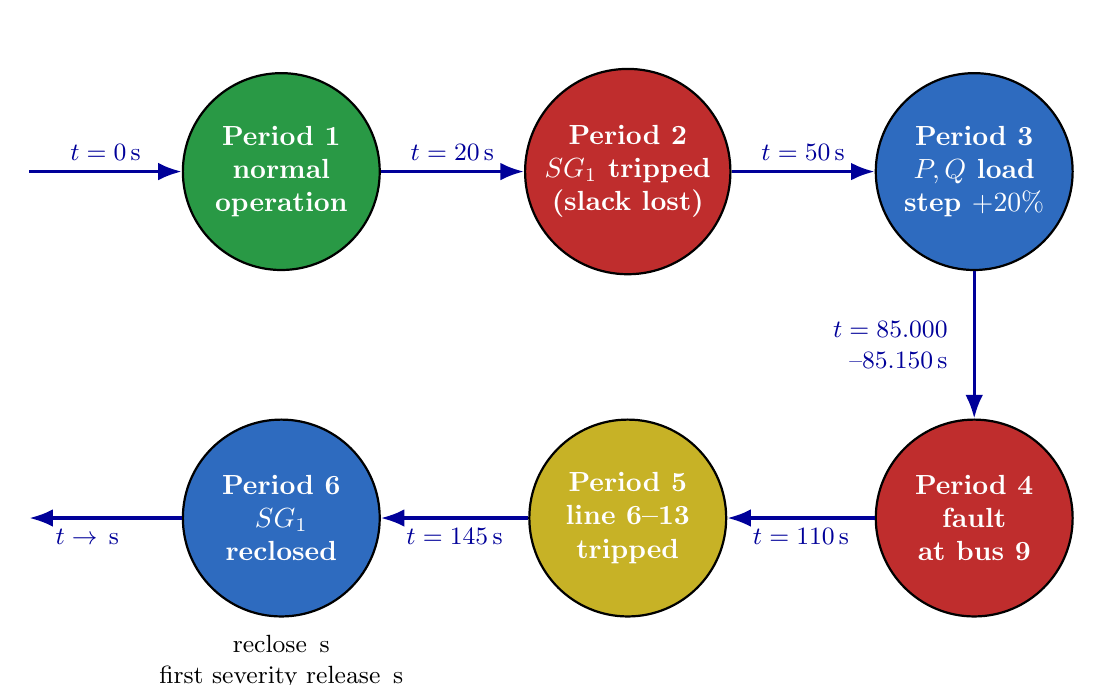
\begin{tikzpicture}[
  font=\normalsize,
  per/.style={circle,draw,thick,minimum size=2.5cm,inner sep=2pt,
    align=center,text=white,font=\bfseries},
  tlbl/.style={font=\small},
  tlab/.style={midway,above,font=\small},
  tlabb/.style={midway,below,font=\small},
  arr/.style={-{Latex[length=3mm]},very thick,color=blue!60!black}]

\node[per,fill=pgreen] (p1) at (0,0)     {Period 1\\ normal\\ operation};
\node[per,fill=pred]   (p2) at (4.4,0)   {Period 2\\ $SG_1$ tripped\\ (slack lost)};
\node[per,fill=pblue]  (p3) at (8.8,0)   {Period 3\\ $P,Q$ load\\ step $+20\%$};
\node[per,fill=pred]   (p4) at (8.8,-4.4){Period 4\\ fault\\ at bus 9};
\node[per,fill=pyellow](p5) at (4.4,-4.4){Period 5\\ line 6--13\\ tripped};
\node[per,fill=pblue]  (p6) at (0,-4.4)  {Period 6\\ $SG_1$\\ reclosed};

\draw[arr] (-3.2,0) -- node[tlab]{$t=0\second$} (p1);
\draw[arr] (p1) -- node[tlab]{$t=20\second$} (p2);
\draw[arr] (p2) -- node[tlab]{$t=50\second$} (p3);
\draw[arr] (p3) -- node[font=\small,left=2mm,pos=0.5,align=right]{$t=85.000$\\--$85.150\second$} (p4);
\draw[arr] (p4) -- node[tlabb]{$t=110\second$} (p5);
\draw[arr] (p5) -- node[tlabb]{$t=145\second$} (p6);
\draw[arr] (p6) -- node[tlabb,pos=0.62]{$t\to\NewRunEnd\second$} ++(-3.2,0);

\node[tlbl,below=3pt of p6,align=center,text=black]
  {reclose $\NewRunReclose\second$\\ first severity release $\NewRunFirstRelease\second$};
\end{tikzpicture}
\caption{Six-period disturbance chronology. Green: undisturbed. Red: a
contingency that removes a source or faults a bus. Yellow: a topology change.
Blue: a restorative action. Scheduled instants ($0$, $20$, $50$,
$85.000$--$85.150$, $110$, $145\second$) are case-defined; the reclose and
first severity-release instants are read from the accepted event log.}
\label{fig:periods}
\end{figure}

Table~\ref{tab:runscalars} collects the summary scalars of the run that draws
every figure in this section. Each is an accepted value of the
$\NewRunEnd\second$ adaptive arm, read through a generated macro rather than typed
into the prose. The voltage and frequency extremes are \emph{reported results} of
a deliberately severe event sequence, not acceptance criteria, and no model was
adjusted after they were seen.

\begin{table}[H]
\centering\footnotesize
\caption{Accepted summary scalars of the $\NewRunEnd\second$ run that draws the
figures of this section.}
\label{tab:runscalars}
\begin{tabularx}{\textwidth}{@{}>{\raggedright\arraybackslash}p{0.38\textwidth}l X@{}}
\toprule
Quantity & Value & Note \\ \midrule
Last accepted time & $\NewRunEnd\second$ & full horizon; no truncation \\
Reclose outcome & \NewRunRecloseStatus & read from the accepted event log \\
Network voltage range & $\NewRunVMin$--$\NewRunVMax\pu$ & transient extrema, not ratings \\
COI frequency range & $\NewRunFMin$--$\NewRunFMax$~Hz & fault and switching window \\
Terminal COI frequency & $\NewRunTerminalF$~Hz & at $t=\NewRunEnd\second$ \\
Terminal voltage range & $\NewRunTerminalVMin$--$\NewRunTerminalVMax\pu$ & at $t=\NewRunEnd\second$ \\
Largest accepted step residual & \NewRunResidual & below the $10^{-8}$ gate at every step \\
Deepest step subdivision & $\NewRunSubdivision$ levels & bisection mechanism \\
Domain-rejected trial steps & $\NewRunDomainRejects$ & no gate was relaxed to pass \\
Controller-rejected steps & $\NewRunRejectedSteps$ & \NewRunStepper\ stepper \\
Accepted samples & $\NewRunSamples$ & \\
SG reclose instant & $\NewRunReclose\second$ & outcome, not a schedule \\
Closing mismatch & $\Delta V=\NewRunSyncDV\pu$ & within the existing synchronism frame \\
 & $\Delta f=$ \NewRunSyncDF\ pu & \\
 & $\Delta\theta=\NewRunSyncDTheta^{\circ}$ & \\
Mode augmentations ($\NewRunNAugment$) &
$\NewRunAugmentOne$, $\NewRunAugmentTwo$, & each passed a transition certificate \\
 & $\NewRunAugmentThree$, $\NewRunAugmentFour\second$ & \\
Mode releases ($\NewRunNRelease$) &
$\NewRunReleaseOne$, $\NewRunReleaseTwo$, & one device at a time \\
 & $\NewRunReleaseThree\second$ & \\
Maximum simultaneous GFM units & $\NewRunGfmMax$ & reached in stages, not at once \\
Post-reclose reselection status & \NewRunReselection & a correct fail-closed outcome \\
\bottomrule
\end{tabularx}
\end{table}

Figure~\ref{fig:pq} reads top to bottom as cause and then effect. Panel~(a) is the
severity index $S$ of Section~\ref{sec:sev} with both thresholds drawn, one trace
per converter because $J_V$ is each converter's own terminal deviation; it is the
only quantity on the page that \emph{causes} anything. Immediately below it are
two supervisory strips: each IBR's grid-forming/grid-following mode, and the
\emph{reference owner} --- the single device that holds the island angle reference
at each instant. Panels~(b) and~(c) are the per-converter active and reactive
power over the full horizon $0\text{--}\NewRunEnd\second$. Mode and reference
ownership are distinct contracts: several IBRs can be grid-forming at once, but
only one of them owns the reference. Here the SG owns it up to $t=20\second$ and
again after the reclose; in between, IBR$_1$ (bus~2) is the reference leader.

The point of this result set is in the mode strip: the supervisor does \emph{not}
raise all four converters together. It augments in $\NewRunNAugment$ stages, at
$\NewRunAugmentOne$, $\NewRunAugmentTwo$, $\NewRunAugmentThree$ and
$\NewRunAugmentFour\second$, until it holds $\NewRunGfmMax$ grid-forming units,
then releases $\NewRunNRelease$ times after the reclose.
Section~\ref{sec:compare} shows that \emph{pinning} those same $\NewRunGfmMax$
units from the trip onwards destroys the run before the horizon, even though that
set passes the linear admissibility check. The order in which the set is reached
therefore matters as much as the set itself.

\clearpage
\begin{figure}[H]
\centering
\IfFileExists{figures/switch_ieee14_decision/mode_switch_PQ.png}
 {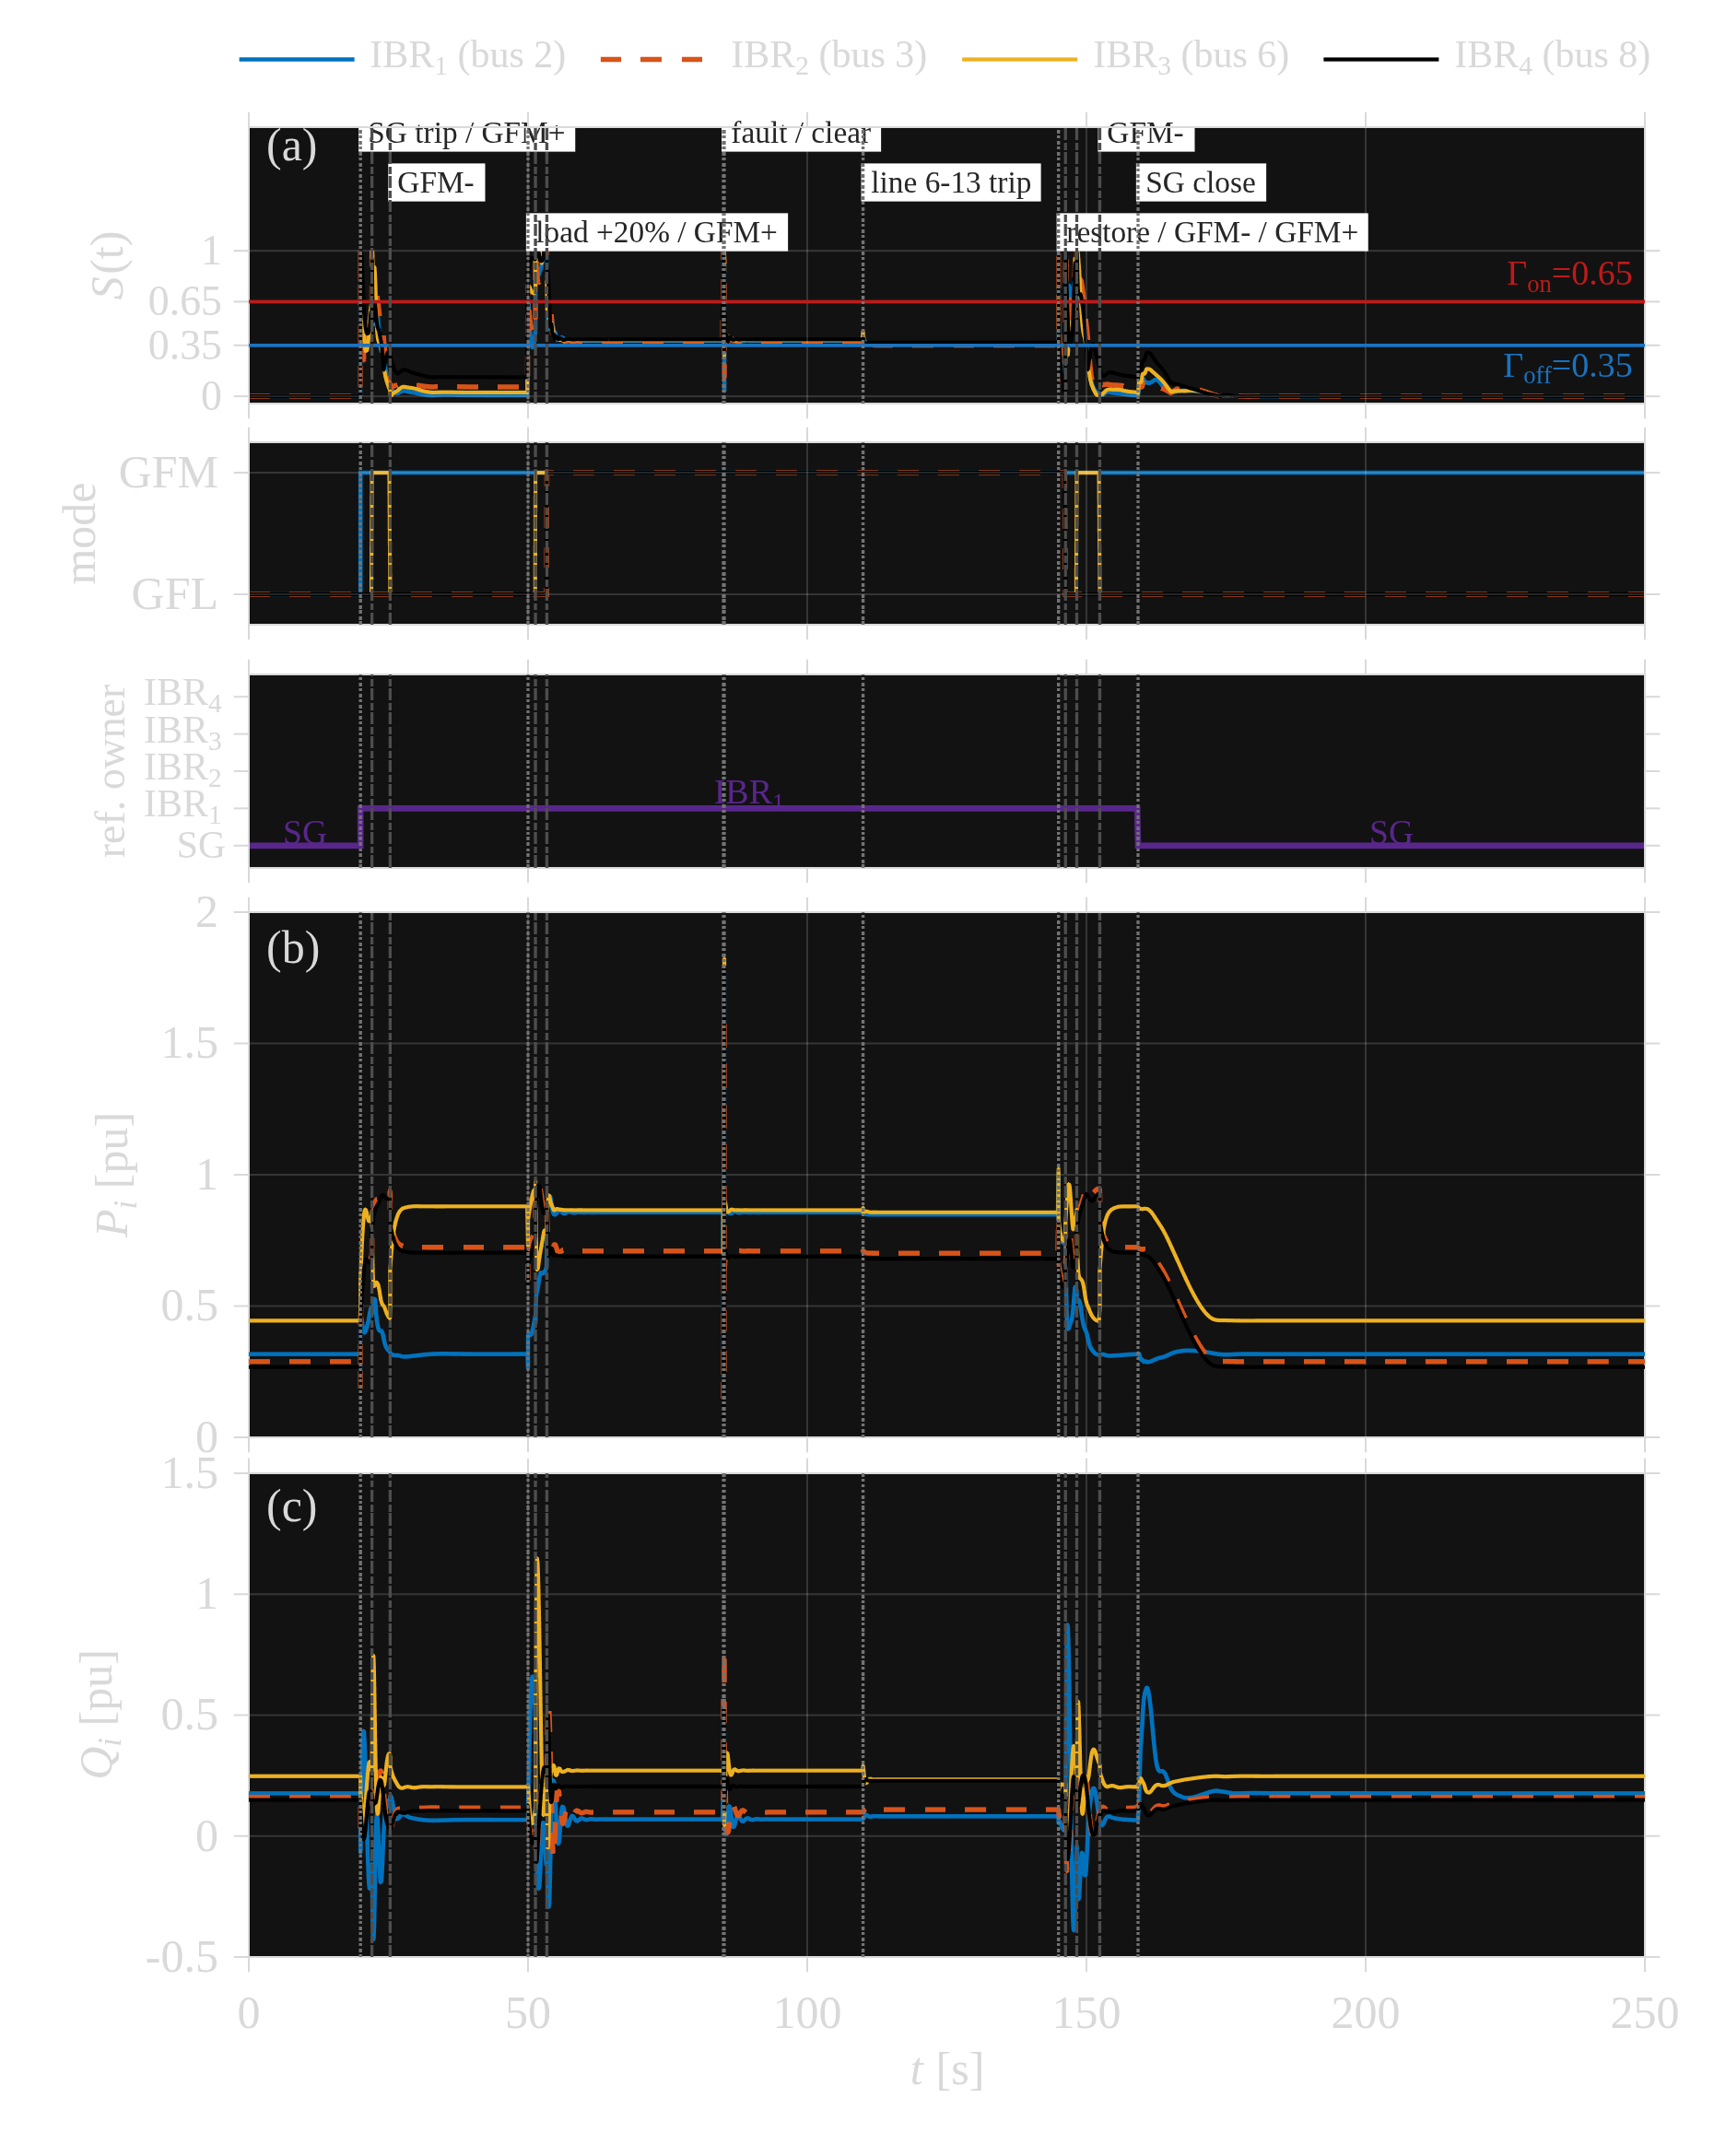
\includegraphics[width=6.20in]{figures/switch_ieee14_decision/mode_switch_PQ.png}}
 {\fbox{\parbox{6.0in}{\centering\vspace{3em}\ttfamily mode\_switch\_PQ.png\\[4pt]
   \normalfont pending figure regeneration
   (run \texttt{generate\_ieee14\_mode\_pq\_figure}).\vspace{3em}}}}
\caption{(a) Severity index $S$ per converter with both switching thresholds,
$\Gamma_{\mathrm{on}}=0.65$ and $\Gamma_{\mathrm{off}}=0.35$. Second strip:
grid-forming or grid-following mode of each IBR. Third strip: the single device
holding the island angle reference. (b) Per-IBR active power $P_i$.
(c) Per-IBR reactive power $Q_i$, both per unit. Dotted lines are scheduled
disturbances and dash--dotted lines the supervisor's own commitments;
near-coincident instants share one label. Raw accepted samples over the full
$\NewRunEnd\second$ horizon.}
\label{fig:pq}
\end{figure}

Figure~\ref{fig:elec} widens the same trajectory into the eight electrical
quantities that the device reconstruction publishes. Panel~(h) is a
whole-network scalar and therefore has one trace by definition; every other panel
carries the four converters and, where a synchronous counterpart exists, the SG.

\clearpage
\begin{figure}[H]
\centering
\IfFileExists{figures/switch_ieee14_decision/electrical_adaptive.png}
 {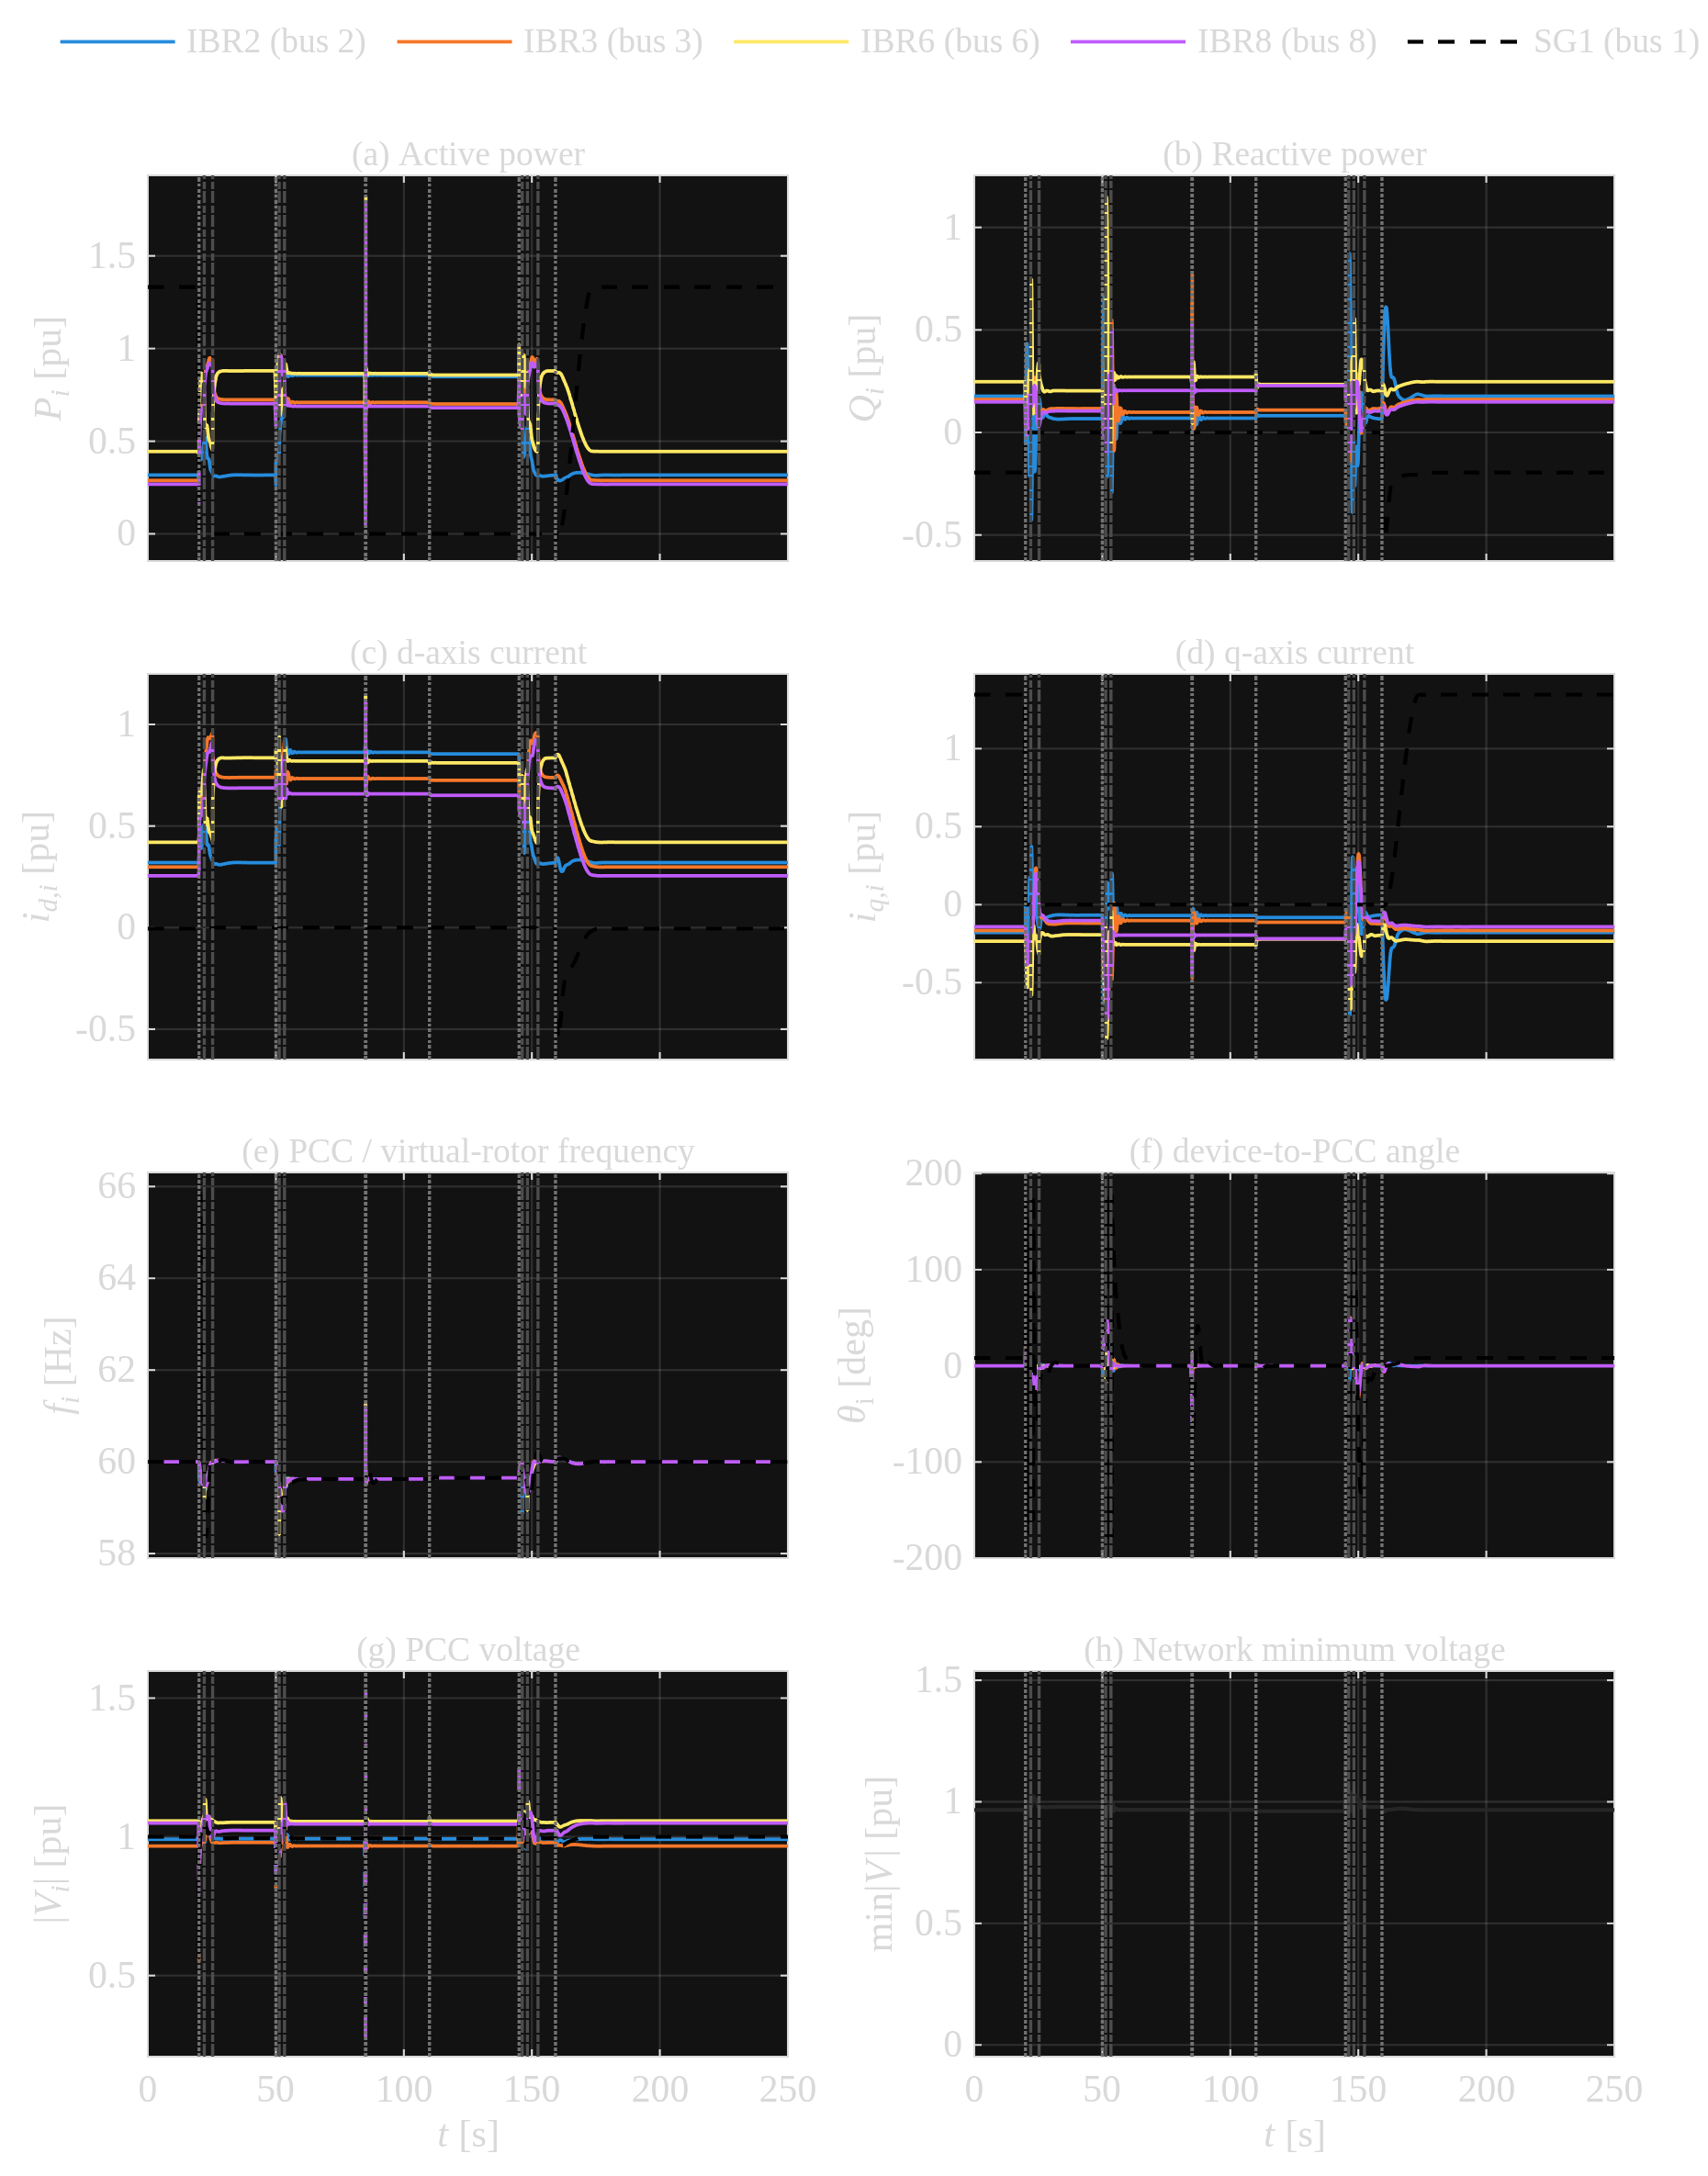
\includegraphics[width=6.20in]{figures/switch_ieee14_decision/electrical_adaptive.png}}
 {\fbox{\parbox{6.0in}{\centering\vspace{3em}\ttfamily electrical\_adaptive.png\\[4pt]
   \normalfont pending figure regeneration
   (run \texttt{generate\_ieee14\_switch\_evidence}).\vspace{3em}}}}
\caption{Eight-panel electrical response over the full $\NewRunEnd\second$
horizon. (a) active power; (b) reactive power; (c) $d$-axis current;
(d) $q$-axis current; (e) PCC or virtual-rotor frequency; (f) device-to-PCC
angle; (g) PCC voltage; (h) network minimum voltage. The SG is dashed black
wherever a synchronous counterpart exists; panel~(h) is a system scalar and has a
single trace by definition. Vertical lines mark the same instants as
Figure~\ref{fig:pq}, unlabelled here because each panel is half a page wide.
Raw accepted samples.}
\label{fig:elec}
\end{figure}

%=============================================================================
\section{Control-policy comparison}\label{sec:compare}
%=============================================================================
The same trajectory is run five times with the \emph{same} network, dispatch,
event schedule, solver and step controller, changing only the IBR control
policy. The runner declares which option fields each arm may differ in and
checks that the structure it built differs from the shared base in no other
field. All five arms are bit-identical on $[0,\CommonWindowSplit)\second$, before
the first event, with $\max|\Delta x|=\max|\Delta y|=\max|\Delta u|=0$ over the
$\CommonWindowPinnedgfmOneSamples$ shared samples, so every later difference is
an effect of the control policy alone. The figures and tables below are the
result; each caption states what it shows and what may not be concluded from it.

\begin{table}[H]
\centering\footnotesize
\caption{Outcome of five control policies on the same $\NewRunEnd\second$
trajectory. A \textbf{--} means the quantity is meaningless for that arm, not that
it is zero.}
\label{tab:arms}
\begin{tabularx}{\textwidth}{@{}>{\raggedright\arraybackslash}p{0.20\textwidth}
  rrrl X@{}}
\toprule
Control policy & Reached [s] & Reclose [s] & Max GFM & Refused by & Outcome \\ \midrule
all IBRs locked GFL &
$\ArmLockedgflHorizon$ & \ArmLockedgflReclose & $\ArmLockedgflGfmMax$ &
\ArmLockedgflFailure &
island left with no voltage-forming source; refused before Newton runs \\
1 GFM pinned (IBR$_1$) &
$\ArmPinnedgfmOneHorizon$ & $\ArmPinnedgfmOneReclose$ & $\ArmPinnedgfmOneGfmMax$ &
\ArmPinnedgfmOneFailure &
survives the horizon, but carries the whole imbalance alone \\
2 GFM pinned (IBR$_2$+IBR$_3$) &
$\ArmPinnedgfmTwoHorizon$ & $\ArmPinnedgfmTwoReclose$ & $\ArmPinnedgfmTwoGfmMax$ &
\ArmPinnedgfmTwoFailure &
survives the horizon; best-damped set in the table \\
all 4 GFM pinned &
$\ArmPinnedgfmFourHorizon$ & \ArmPinnedgfmFourReclose & $\ArmPinnedgfmFourGfmMax$ &
\ArmPinnedgfmFourFailure &
\textbf{fails before the horizon}, although this set is linearly admissible \\
automatic switching (delivered) &
$\ArmAdaptiveHorizon$ & $\ArmAdaptiveReclose$ & $\ArmAdaptiveGfmMax$ &
\ArmAdaptiveFailure &
survives the horizon \emph{and} reaches the four-unit set \\
\bottomrule
\end{tabularx}
\end{table}

\clearpage
\begin{figure}[H]
\centering
\IfFileExists{figures/switch_ieee14_decision/comparison_switch_vs_lock.png}
 {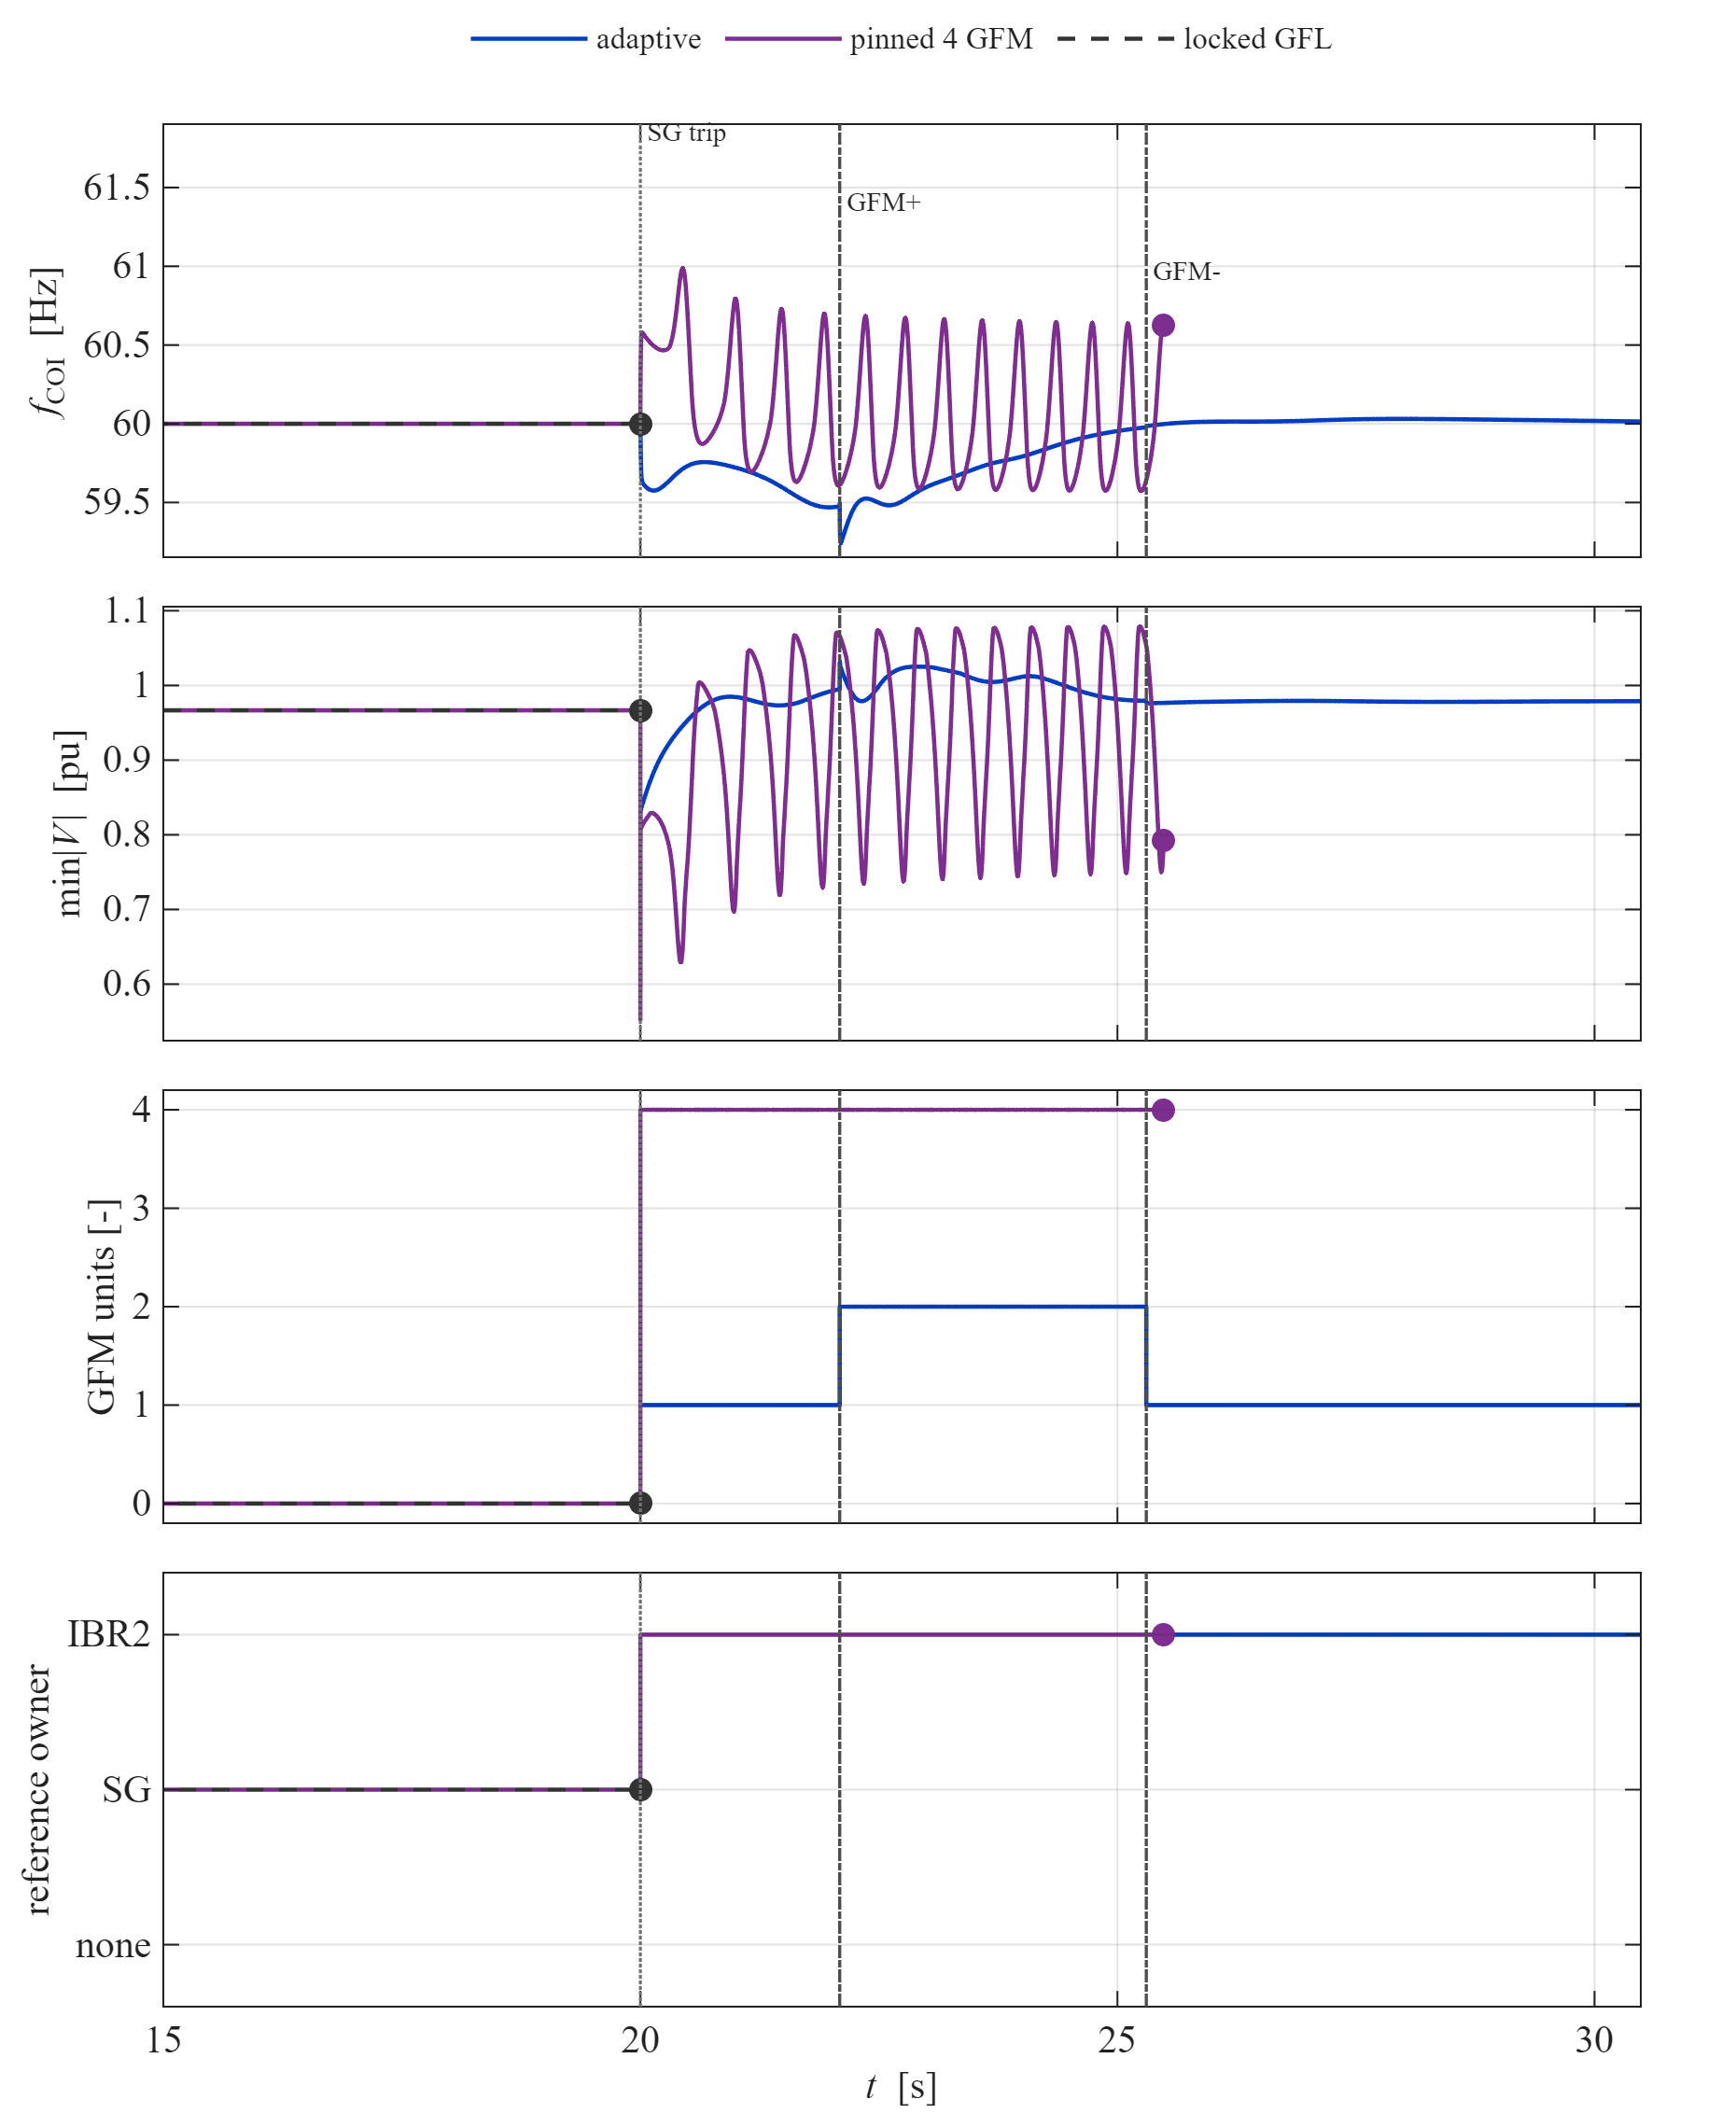
\includegraphics[width=6.20in]{figures/switch_ieee14_decision/comparison_switch_vs_lock.png}}
 {\fbox{\parbox{6.0in}{\centering\vspace{2em}\ttfamily
   comparison\_switch\_vs\_lock.png\\[4pt]\normalfont
   pending figure regeneration.\vspace{2em}}}}
\caption{Switching against not switching, in the window where the two part
company. Rows, top to bottom: centre-of-inertia frequency, network minimum
voltage, number of grid-forming units, and which device holds the island angle
reference. \textbf{Switching} (solid) rides through the loss of the synchronous
machine and continues to the end of the horizon. \textbf{All four units pinned
grid-forming} from the outset, with no run-time switching, breaks into a growing
oscillation and the trajectory ends at
$t=\ArmPinnedgfmFourHorizon\second$ with \ArmPinnedgfmFourFailure; the terminating
sample is marked, and the curve is not continued past it. \textbf{All units
locked grid-following} cannot be integrated at all past the trip: the island is
left with no voltage-forming source, the per-island admissibility gate refuses
the transaction before Newton is called even once, and the trajectory ends at the
left-limit sample of the event, exactly $t=\ArmLockedgflHorizon\second$. An arm
that ends early is never extended to match the others, and no quantity is
reported for an arm over an interval it did not reach.}
\label{fig:swlock}
\end{figure}

\clearpage
\begin{figure}[H]
\centering
\IfFileExists{figures/switch_ieee14_decision/comparison_full.png}
 {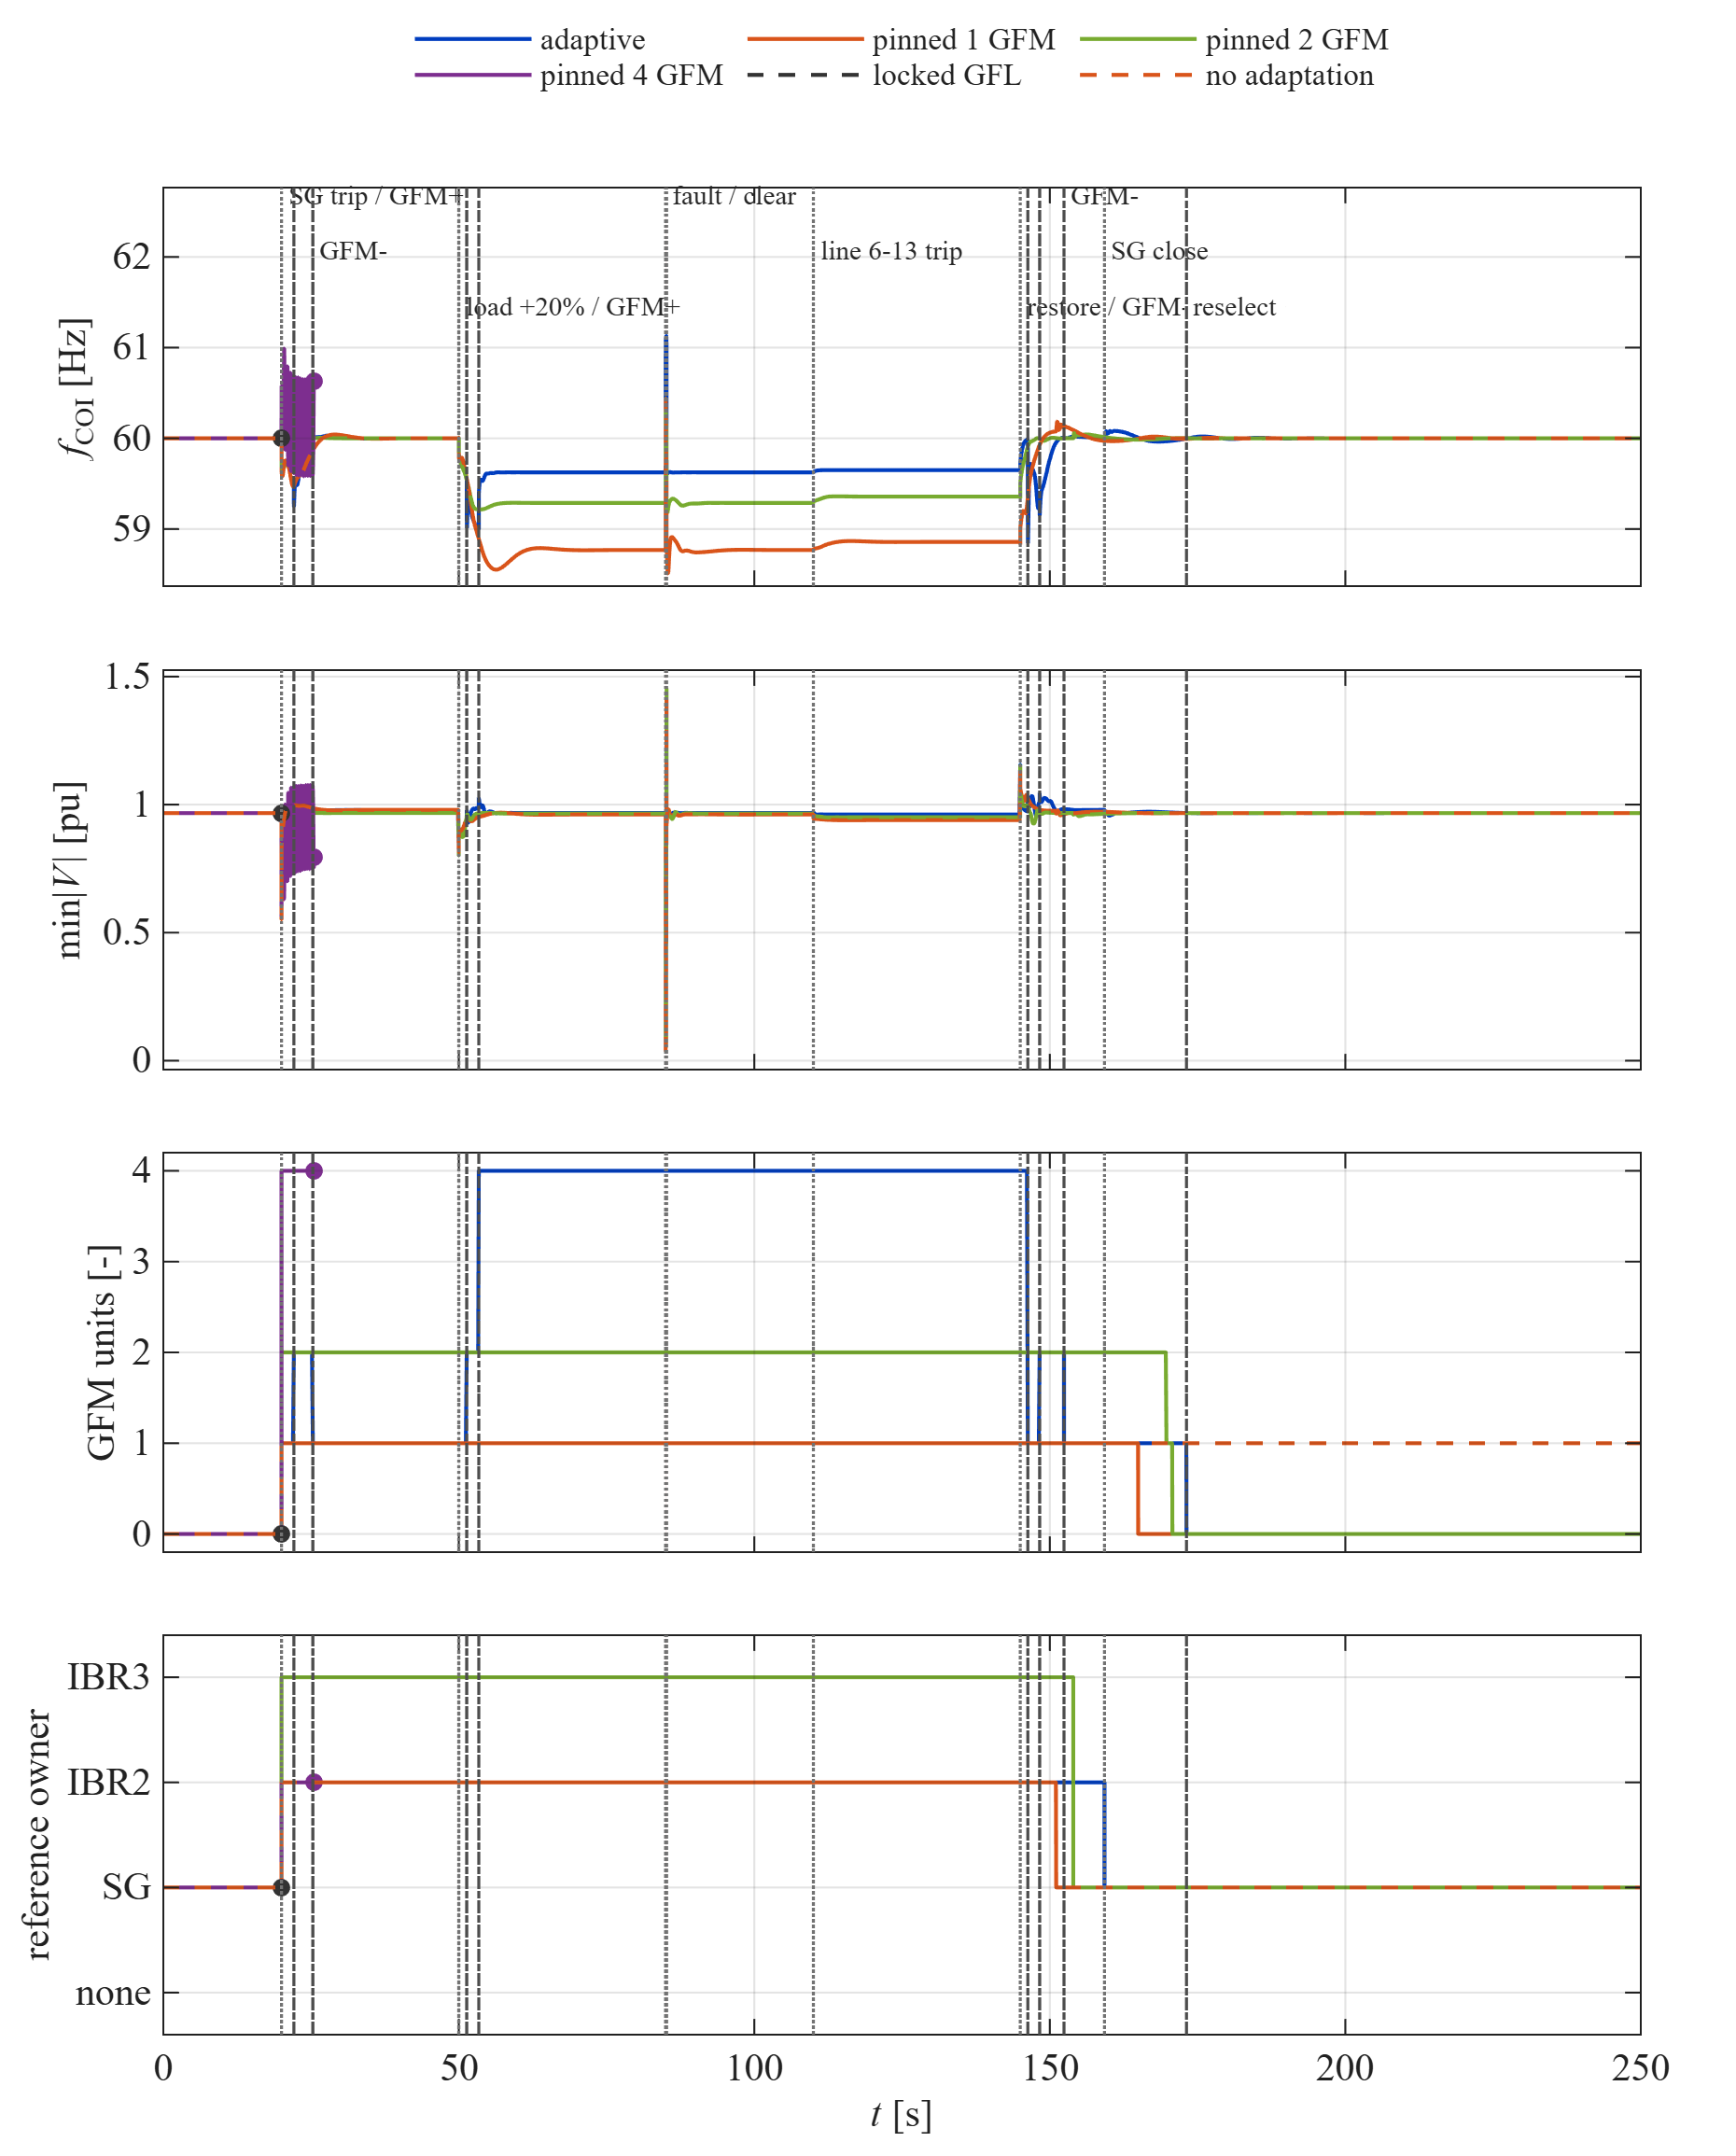
\includegraphics[width=6.20in]{figures/switch_ieee14_decision/comparison_full.png}}
 {\fbox{\parbox{6.0in}{\centering\vspace{2em}\ttfamily comparison\_full.png\\[4pt]
   \normalfont pending figure regeneration.\vspace{2em}}}}
\caption{Five arms overlaid over the full horizon. Rows top to bottom:
centre-of-inertia frequency, network minimum voltage, number of grid-forming
units, and reference-angle owner. The chronology is named once, on the top row,
in a band reserved above the data. This page reads the \emph{settled} behaviour:
the three surviving arms separate into three distinct frequency levels, and the
staged $1\!\to\!2\!\to\!4$ progression of the switching arm is visible in the
third row. An arm that ends before the horizon stops at its own last accepted
sample (solid marker) and is \emph{not} extended, held, or extrapolated to match
the others. Every y range is taken from the data actually inside the plotted time
window, and the generator aborts if any sample would fall outside it.}
\label{fig:cmparms}
\end{figure}

\clearpage
\begin{figure}[H]
\centering
\IfFileExists{figures/switch_ieee14_decision/comparison_windows.png}
 {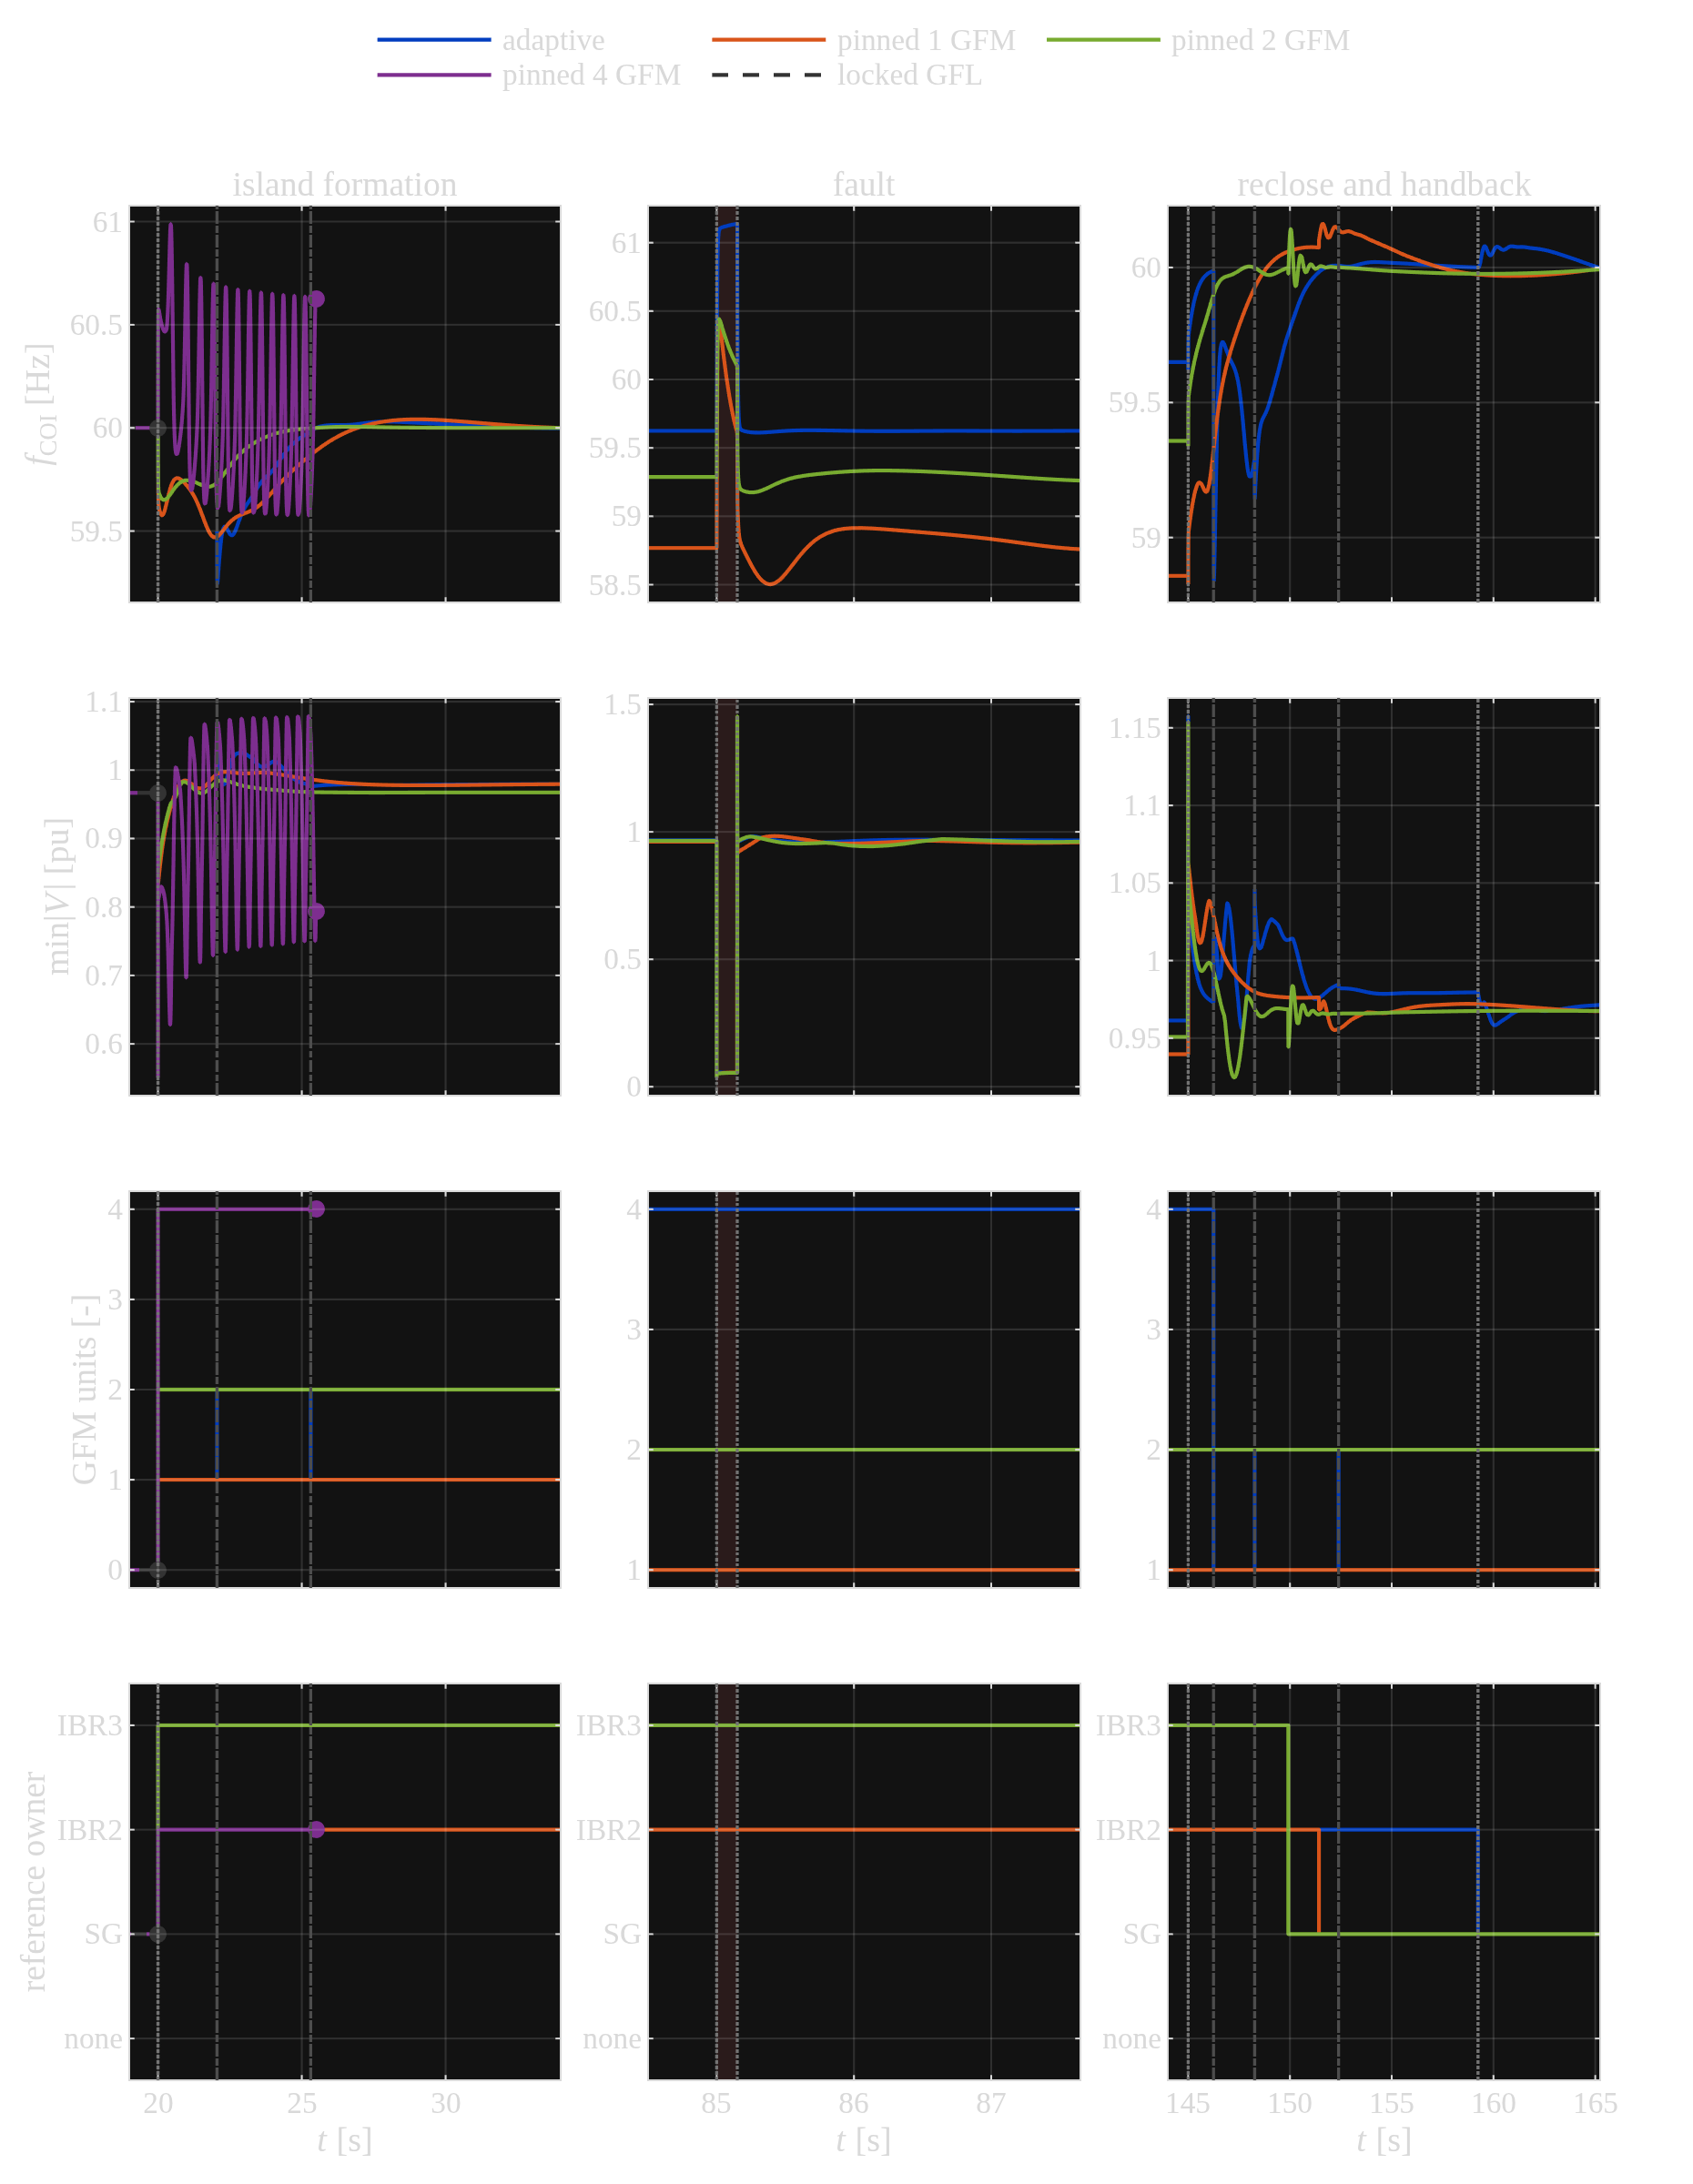
\includegraphics[width=6.20in]{figures/switch_ieee14_decision/comparison_windows.png}}
 {\fbox{\parbox{6.0in}{\centering\vspace{2em}\ttfamily comparison\_windows.png\\[4pt]
   \normalfont pending figure regeneration.\vspace{2em}}}}
\caption{The same four rows over the three windows in which the transients are
resolvable, every bound derived from the event schedule. Left: island formation,
where the pinned four-unit arm breaks into a growing oscillation and terminates.
Centre: the fault, with the $0.150$~s shunt interval shaded, showing the network
minimum voltage collapsing and recovering. Right: reclose and hand-back. Each
column is scaled to its own window, which is what the previous single-page version
failed to do.}
\label{fig:cmpwin}
\end{figure}

\begin{table}[H]
\centering\footnotesize
\caption{Frequency deviation in the 15-second window after each event, for the
three arms that reach the horizon. Peak is $\max|f_{COI}-60|$; settled is the mean
of $|f_{COI}-60|$ over the last 30\% of the window. All values in hertz.}
\label{tab:excursion}
\begin{tabular}{lrrr|rrr}
\toprule
& \multicolumn{3}{c|}{Peak} & \multicolumn{3}{c}{Settled} \\
Event & 1 GFM & 2 GFM & switching & 1 GFM & 2 GFM & switching \\ \midrule
SG trip ($20\second$) &
$\DfPinnedgfmOneSGtrip$ & $\DfPinnedgfmTwoSGtrip$ & $\DfAdaptiveSGtrip$ &
$\SetPinnedgfmOneSGtrip$ & $\SetPinnedgfmTwoSGtrip$ & $\SetAdaptiveSGtrip$ \\
load $+20\%$ ($50\second$) &
$\DfPinnedgfmOneLoadstep$ & $\DfPinnedgfmTwoLoadstep$ & $\DfAdaptiveLoadstep$ &
$\SetPinnedgfmOneLoadstep$ & $\SetPinnedgfmTwoLoadstep$ & $\SetAdaptiveLoadstep$ \\
fault ($85\second$) &
$\DfPinnedgfmOneFault$ & $\DfPinnedgfmTwoFault$ & $\DfAdaptiveFault$ &
$\SetPinnedgfmOneFault$ & $\SetPinnedgfmTwoFault$ & $\SetAdaptiveFault$ \\
line 6--13 open ($110\second$) &
$\DfPinnedgfmOneLinetrip$ & $\DfPinnedgfmTwoLinetrip$ & $\DfAdaptiveLinetrip$ &
$\SetPinnedgfmOneLinetrip$ & $\SetPinnedgfmTwoLinetrip$ & $\SetAdaptiveLinetrip$ \\
reclose ($145\second$) &
$\DfPinnedgfmOneRestorereclose$ & $\DfPinnedgfmTwoRestorereclose$ &
$\DfAdaptiveRestorereclose$ &
$\SetPinnedgfmOneRestorereclose$ & $\SetPinnedgfmTwoRestorereclose$ &
$\SetAdaptiveRestorereclose$ \\
\bottomrule
\end{tabular}
\end{table}

\begin{figure}[H]
\centering
\IfFileExists{figures/switch_ieee14_decision/comparison_event_excursions.png}
 {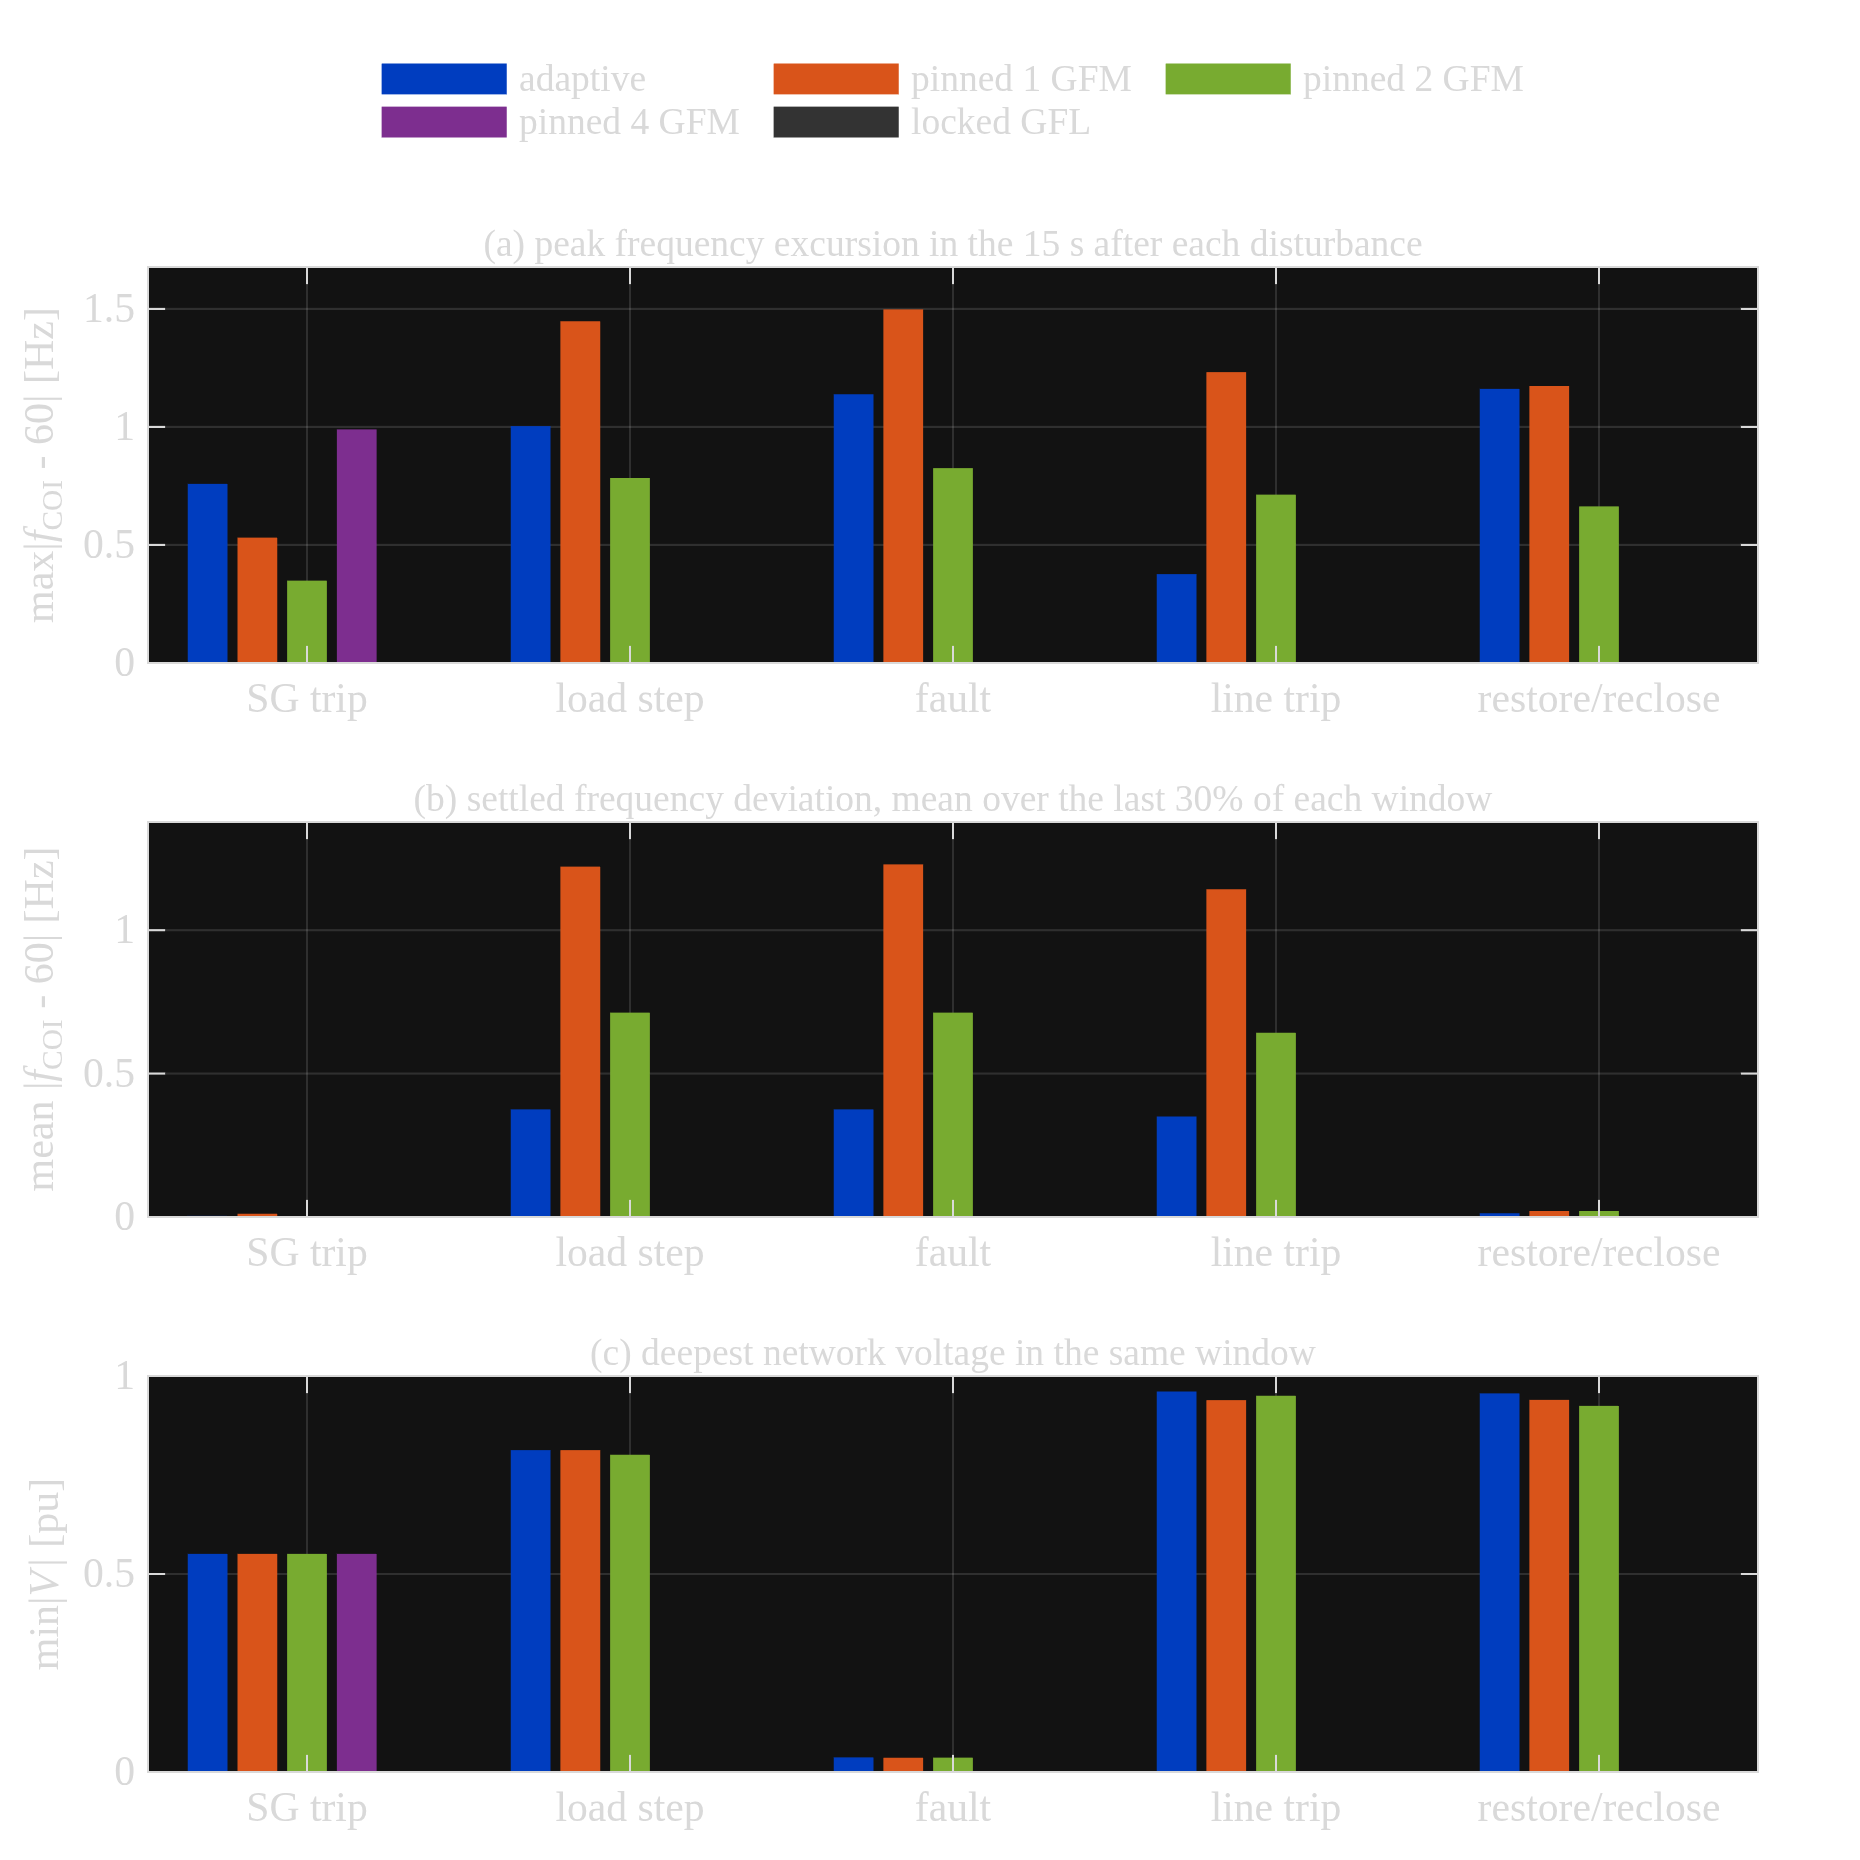
\includegraphics[width=6.20in]{figures/switch_ieee14_decision/comparison_event_excursions.png}}
 {\fbox{\parbox{6.0in}{\centering\vspace{2em}\ttfamily
   comparison\_event\_excursions.png\\[4pt]\normalfont
   pending figure regeneration.\vspace{2em}}}}
\caption{(a) Peak frequency deviation in the 15-second window after each event.
(b) Settled deviation in the same window. (c) Network minimum voltage. A missing
bar means that arm never entered that window; it does not mean zero.}
\label{fig:cmpbars}
\end{figure}

\IfFileExists{figures/switch_ieee14_decision/sg_off_admissibility.tex}
 {% Generated by generate_ieee14_gfm_lock_comparison. Do not edit.
\begin{table}[H]\centering\footnotesize
\caption{Every candidate grid-forming subset for the islanded (SG-off) band, screened before the run. $\Omega$ is the damping margin of that configuration's own equilibrium; a more negative value is better damped. The admissible set is \emph{not} monotone in the number of grid-forming units, and the best two-unit configuration is better damped than all four.}
\begin{tabular}{llcrl}\toprule
\label{tab:cand}%
grid-forming set & reference & $n$ & $\Omega$ & outcome \\ \midrule
IBR8 & IBR8 & 1 & -0.15544 & admissible \\
IBR6 & IBR6 & 1 & -0.25203 & admissible \\
IBR3 & IBR3 & 1 & -0.31671 & admissible \\
IBR2 & IBR2 & 1 & -0.32801 & admissible \\
IBR2+IBR6 & IBR2 & 2 & -0.56172 & admissible \\
IBR3+IBR6 & IBR3 & 2 & -0.56814 & admissible \\
IBR2+IBR3 & IBR2 & 2 & -- & no equilibrium (IBR6 at a limit) \\
IBR2+IBR8 & IBR2 & 2 & -- & no equilibrium (IBR6 at a limit) \\
IBR3+IBR8 & IBR3 & 2 & -- & no equilibrium (IBR6 at a limit) \\
IBR6+IBR8 & IBR6 & 2 & -- & no equilibrium (IBR3 at a limit) \\
IBR2+IBR3+IBR6 & IBR2 & 3 & -- & no equilibrium (Newton did not converge) \\
IBR2+IBR3+IBR8 & IBR2 & 3 & -- & no equilibrium (Newton did not converge) \\
IBR2+IBR6+IBR8 & IBR2 & 3 & -- & no equilibrium (Newton did not converge) \\
IBR3+IBR6+IBR8 & IBR3 & 3 & -- & no equilibrium (Newton did not converge) \\
IBR2+IBR3+IBR6+IBR8 & IBR2 & 4 & -0.48291 & admissible \\
\bottomrule\end{tabular}\end{table}

\paragraph{Best authenticated configuration.} IBR3+IBR6, with $n=2$ and $\Omega=-0.56814$. The best singleton reaches $\Omega=-0.32801$ and the full set -0.48291, so the optimum is interior: adding grid-forming units past it degrades the margin. This is a small-signal result about one equilibrium and does not by itself certify the transient response; the arm comparison measures that separately.
}
 {\begin{center}\ttfamily sg\_off\_admissibility.tex pending regeneration
  (run \texttt{generate\_ieee14\_gfm\_lock\_comparison}).\end{center}}

\begin{figure}[H]
\centering
\IfFileExists{figures/switch_ieee14_decision/sg_off_admissibility.png}
 {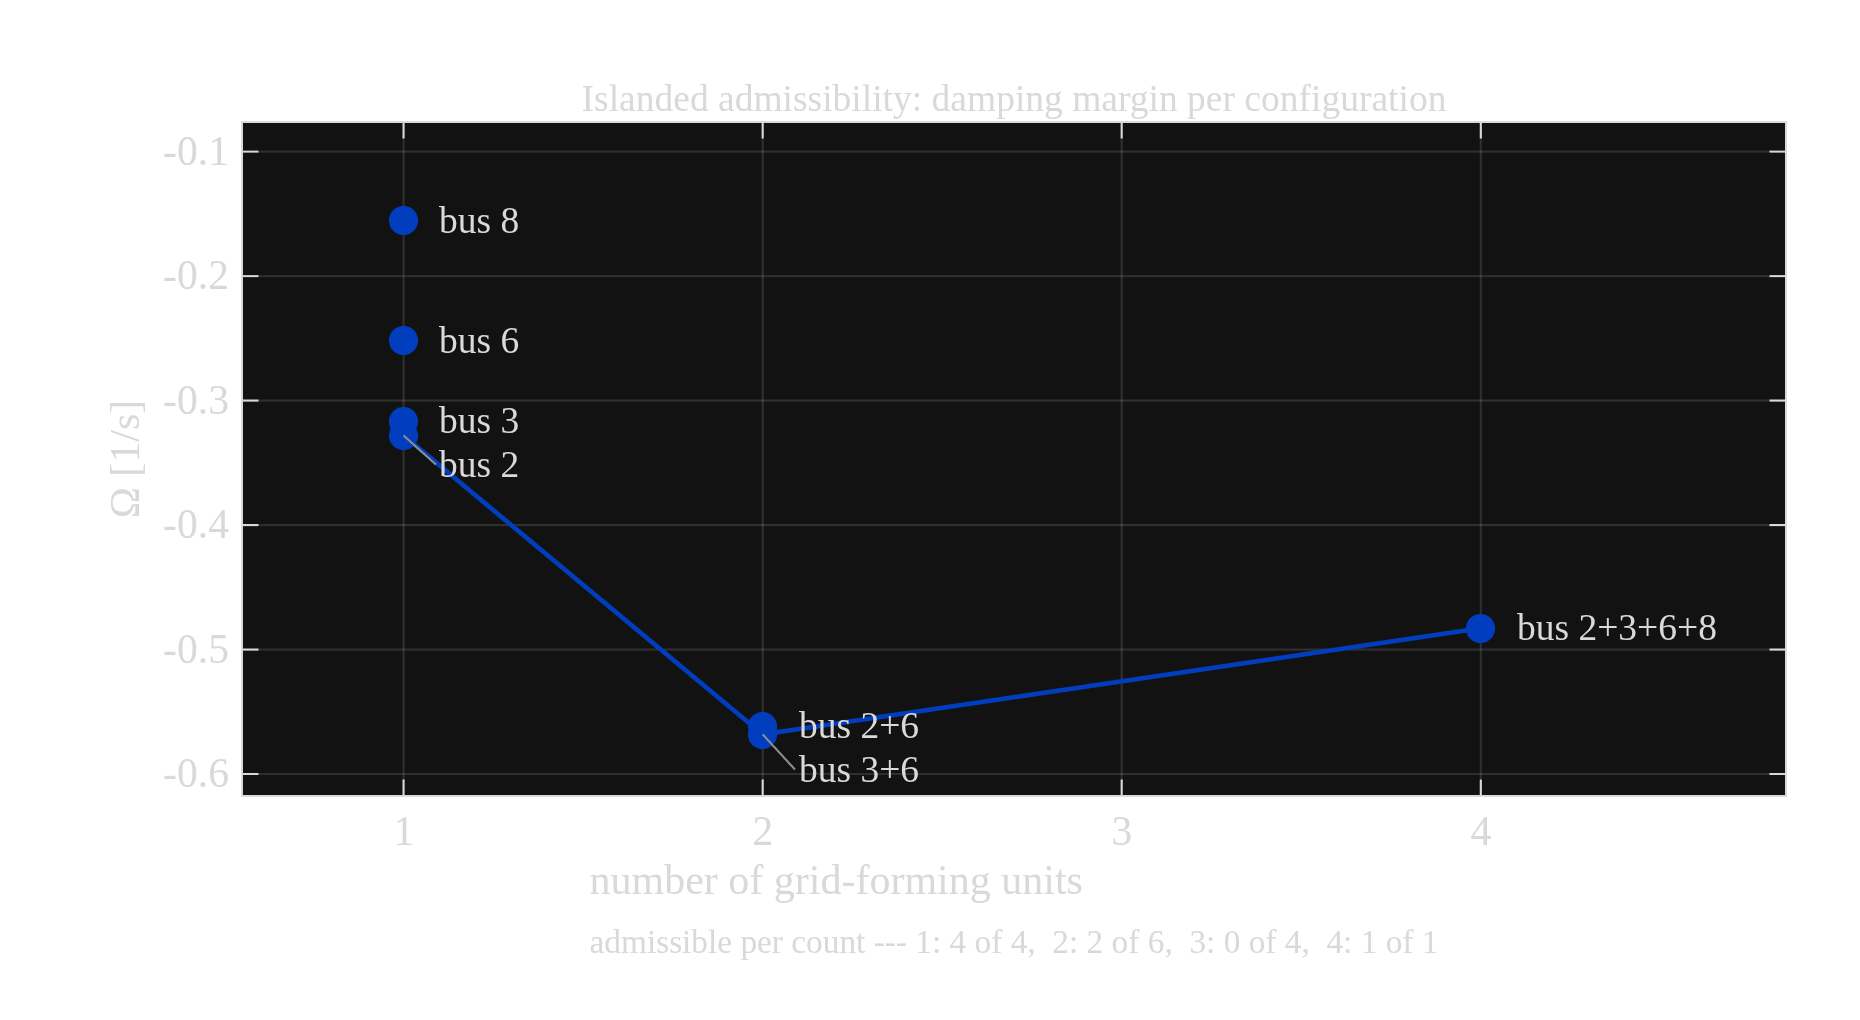
\includegraphics[width=6.20in]{figures/switch_ieee14_decision/sg_off_admissibility.png}}
 {\fbox{\parbox{6.0in}{\centering\vspace{2em}\ttfamily
   sg\_off\_admissibility.png\\[4pt]\normalfont
   pending figure regeneration.\vspace{2em}}}}
\caption{Damping margin $\Omega$ of every \emph{admissible} grid-forming
configuration, each at its own measured value, against the number of units (more
negative is better damped). The connecting line follows the best configuration at
each cardinality, which makes the interior optimum at two units immediate. Labels
are separated in point space with leader lines where two margins differ by less
than one line of type. The configurations with no equilibrium are \emph{not}
plotted: a marker at a position that is not its value cannot be measured off the
axis. Their count at each cardinality is printed under the axis and their
individual reasons are in Table~\ref{tab:cand}.}
\label{fig:cand}
\end{figure}

\begin{thebibliography}{99}
%-----------------------------------------------------------------------------
% Every entry below was verified against the document it names: author list,
% venue, volume, issue and year from the article front matter, and the page range
% confirmed by checking that the computed last page actually appears on the last
% page of the document. Where a range could not be confirmed it is omitted rather
% than computed, and pre-publication items are marked as such.
%-----------------------------------------------------------------------------
\bibitem{ieee1110} IEEE Std 1110-2002, \emph{IEEE Guide for Synchronous Generator
Modeling Practices and Applications in Power System Stability Analyses}.

\bibitem{kundur1994} P.~Kundur, \emph{Power System Stability and Control}. New
York: McGraw-Hill, 1994.

\bibitem{sauerpai1998} P.~W.~Sauer and M.~A.~Pai, \emph{Power System Dynamics and
Stability}. Upper Saddle River, NJ: Prentice Hall, 1998.

\bibitem{kodsi2003} S.~K.~M.~Kodsi and C.~A.~Ca\~{n}izares, ``Modeling and
simulation of IEEE 14 bus system with FACTS controllers,'' Univ.\ of Waterloo
Technical Report 2003-3, 2003. (Machine dynamic data, Table~A.2.)

\bibitem{matpower} MATPOWER case \texttt{case14}, IEEE 14-bus test case converted
from the IEEE common data format, as distributed with the MATPOWER package. Used
here for network topology, branch data and the load schedule.

\bibitem{yazdani2010} A.~Yazdani and R.~Iravani, \emph{Voltage-Sourced Converters
in Power Systems: Modeling, Control, and Applications}. Hoboken, NJ: Wiley/IEEE
Press, 2010, ISBN 978-0-470-52156-4.

\bibitem{teodorescu2011} R.~Teodorescu, M.~Liserre, and P.~Rodr\'{i}guez,
\emph{Grid Converters for Photovoltaic and Wind Power Systems}. Chichester, UK:
Wiley/IEEE Press, 2011, ISBN 978-0-470-05751-3.

\bibitem{bacha2014} S.~Bacha, I.~Munteanu, and A.~I.~Bratcu, \emph{Power
Electronic Converters Modeling and Control}. London: Springer, 2014,
doi:10.1007/978-1-4471-5478-5.

\bibitem{pogaku2007} N.~Pogaku, M.~Prodanovi\'{c}, and T.~C.~Green, ``Modeling,
analysis and testing of autonomous operation of an inverter-based microgrid,''
\emph{IEEE Trans.\ Power Electron.}, vol.~22, no.~2, pp.~613--625, 2007.

\bibitem{sakimoto2015} K.~Sakimoto, Y.~Miura, and T.~Ise, ``Virtual synchronous
generator without phase locked loop based on current controlled inverter and its
parameter design,'' \emph{IEEJ Trans.\ Power and Energy}, vol.~135, no.~7,
pp.~462--470, 2015.

\bibitem{regfmb1} National Renewable Energy Laboratory, \emph{REGFM\_B1: An
Electromagnetic Transient Model for Grid-Forming Inverters}, NREL/TP-5D00-90260,
2024.

\bibitem{he2024} C.~He, H.~Geng, K.~Rajashekara, and A.~Chandra, ``Analysis and
control of frequency stability in low-inertia power systems: a review,''
\emph{IEEE/CAA J.\ Autom.\ Sinica}, vol.~11, no.~12, pp.~2363--2383, Dec.\ 2024,
doi:10.1109/JAS.2024.125013.

\bibitem{zhang2025} W.~Zhang, Y.~Wen, and C.~Y.~Chung, ``Inertia security
evaluation and application in low-inertia power systems,'' \emph{IEEE Trans.\
Power Syst.}, vol.~40, no.~2, pp.~1725--1737, Mar.\ 2025,
doi:10.1109/TPWRS.2024.3420786.

\bibitem{nema2022} S.~Nema, V.~Prakash, and H.~Pand\v{z}i\'{c}, ``Adaptive
synthetic inertia control framework for distributed energy resources in
low-inertia microgrid,'' \emph{IEEE Access}, vol.~10, 2022,
doi:10.1109/ACCESS.2022.3177661.

\bibitem{cui2025} G.~Cui, Z.~Chu, and F.~Teng, ``Control-mode as a grid service in
software-defined power grids: GFL vs GFM,'' \emph{IEEE Trans.\ Power Syst.},
vol.~40, no.~1, pp.~314--326, Jan.\ 2025, doi:10.1109/TPWRS.2024.3404339.

\bibitem{ding2025} H.~Ding, R.~Kar, Z.~Miao, and L.~Fan, ``A novel design for
switchable grid-following and grid-forming control,'' \emph{IEEE Trans.\ Sustain.\
Energy}, vol.~16, no.~2, pp.~1301--1314, Apr.\ 2025,
doi:10.1109/TSTE.2024.3520989.

\bibitem{liu2024} P.~Liu, X.~Xie, and J.~Shair, ``Adaptive hybrid grid-forming and
grid-following control of IBRs with enhanced small-signal stability under varying
SCRs,'' \emph{IEEE Trans.\ Power Electron.}, vol.~39, no.~6, pp.~6603--6607,
Jun.\ 2024, doi:10.1109/TPEL.2024.3373659.

\bibitem{gao2025} X.~Gao, D.~Zhou, A.~Anvari-Moghaddam, and F.~Blaabjerg,
``Seamless switching method between grid-following and grid-forming control for
renewable energy conversion systems,'' \emph{IEEE Trans.\ Ind.\ Appl.}, vol.~61,
no.~1, pp.~597--606, Jan./Feb.\ 2025.

\bibitem{askarian2024} A.~Askarian, J.~Park, and S.~Salapaka, ``Enhanced
grid-following (E-GFL) inverter: a unified control framework for stiff and weak
grids,'' \emph{IEEE Trans.\ Power Electron.}, vol.~39, no.~5, pp.~5089--5107,
May 2024, doi:10.1109/TPEL.2024.3350528.

\bibitem{he2022} C.~He, X.~He, H.~Geng, H.~Sun, and S.~Xu, ``Transient stability
of low-inertia power systems with inverter-based generation,'' \emph{IEEE Trans.\
Energy Convers.}, vol.~37, no.~4, pp.~2903--2912, Dec.\ 2022,
doi:10.1109/TEC.2022.3185623.

\bibitem{qu2025} Q.~Qu, X.~Xiang, K.~Xin, Y.~Liu, W.~Li, and X.~He, ``Transient
stability analysis of hybrid GFL-GFM system considering various damping effects,''
\emph{IEEE Trans.\ Ind.\ Electron.}, vol.~72, no.~12, pp.~13334--13347,
Dec.\ 2025, doi:10.1109/TIE.2025.3581260.

\bibitem{li2026} B.~Li, S.~Yang, P.~Cheng, and Z.~Hao, ``Transient stability of
GFL converters subjected to switching of droop-controlled GFM converters,''
\emph{IEEE Trans.\ Energy Convers.}, early access,
doi:10.1109/TEC.2026.3676254. (Author's accepted version; content may change
before final publication.)

\bibitem{chen2025} L.~Chen, S.~Zheng, R.~Tao, Z.~Liu, Y.~Li, Y.~Li, Y.~Jiang, and
H.~Chen, ``Transient stability analysis approach of the SG-GFL-GFM parallel system
based on power-angle interaction mechanism,'' \emph{Protection and Control of
Modern Power Systems}, early access, doi:10.23919/PCMP.2025.000197.

\bibitem{almesri2025} Z.~M.~Almesri, H.~A.~Hussain, and R.~M.~Kamel, ``Low voltage
ride-through capability of grid-connected PV systems: a comparative study of
grid-following and grid-forming converters under current limits,'' \emph{IEEE
Access}, vol.~13, pp.~105590--105607, 2025, doi:10.1109/ACCESS.2025.3580643.

\bibitem{nurunnabi2025} M.~Nurunnabi, S.~Li, and H.~S.~Das, ``Advancing
grid-forming inverter technology: comprehensive PQ capability and performance
analysis,'' \emph{IEEE Access}, vol.~13, pp.~73391--73407, 2025,
doi:10.1109/ACCESS.2025.3561788.
\end{thebibliography}

\end{document}
